\chapter{The Search for $\boldmath{t+p_\text{T}^\text{miss}}$}
\label{sec:mt}

In this chapter, we discuss the search for dark matter produced in association with a single top quark (``mono-top'').
Since the initial state of $pp$ collisions do not contain any appreciable contribution from top quarks, any process that produces a single top quark must involve some flavor violation.
In the Standard Model, any such process is heavily suppressed by off-diagonal elements of the CKM matrix.
The SM production mechanism for the mono-top signature (Figure~\ref{fig:mt:tzq}) involves a $b$ quark in the final state, and thus does not couple the third generation with the first or second.
True production of mono-top must introduce some such coupling as an extension to the SM, in addition to one (or more) invisible particle to serve as a DM candidate.

\begin{figure}[]
    \begin{center}
        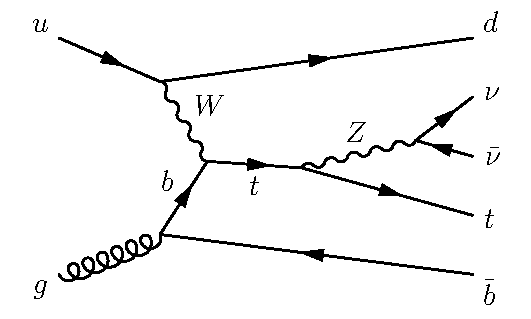
\includegraphics[width=0.5\textwidth]{figures/monotop/diagrams/tzq.pdf}
        \caption{Production of mono-top in the SM, in which a top quark is produced in addition to a $Z$ boson and bottom quark. The $Z$ decays to neutrinos, providing large \ptmiss.}
        \label{fig:mt:tzq}
    \end{center}
\end{figure}

To illustrate how beyond-SM physics can produce this final state, we introduce two DM models: a flavor-changing neutral current $V$ and a charged, colored scalar $\phi$.
These models will also be used to benchmark the sensitivity of the analysis.
However, it should be emphasized that the search is motivitated and designed agnostically, without reliance on any specific model; the assumption is that the mono-top final state alone is indicative of new physics, regardless of the specific production mechanism.

The FCNC $V$ is assumed to couple to a fermionic DM candidate $\chi$. 
A partial Lagrangian of the interaction terms is given by:
\begin{equation}
\mathcal{L}_\text{int}=  V_\mu  \overline\chi \gamma^\mu (  g^V_{\chi} + g^A_{\chi} \gamma_5 ) \chi
                           + \overline{q}_u \gamma^\mu
                           ( g^V_u + g^A_u \gamma_5 ) q_u V_\mu
                           + \overline{q}_{d} \gamma^\mu
                           (  g^V_{d} + g^A_{d} \gamma_5 ) q_d V_\mu
                           + \text{h.c.},
    \label{eq:Lfcnc}
\end{equation}
The model comes with 22 free parameters, broadly organized in three sets:
\begin{itemize}
    \item The masses $m_V$ and $m_\chi$. (2)
    \item The couplings $g_\chi^V$ and $g_\chi^A$. These, respectively, control the strength of the vector and axial interactions between $V$ and $\chi$. (2)
    \item The four coupling matrices $g_{q}^{X}$, where $q=u,d$ and $X=V,A$. 
          As before, $X$ determines the type of spin-1 interaction. 
          In principle, different coupling strengths can be permitted for up- and down-type quarks, so this indexed by $q$. 
          Each $g_{q}^{X}$ is a $3\times3$ matrix, cross-coupling the three quark generations. 
          To preserve $\mathrm{SU}(2)_\mathrm{L}$ symmetry, we require $g_u^V - g_u^A = g_d^V - g_d^A$. ($3\times6=18$)
\end{itemize}

It is the $g_{u,d}^{V,A}$ matrices that determine whether the model can produce mono-top, or mono-bottom, or mono-up, etc. 
If $g_{u,d}$ is strongly diagonal (i.e. strongest couplings are within generations), then mono-light quark production will dominate, resulting in the mono-jet final state (Figure~\ref{fig:mt:fcncdiaga}).
On the other hand, if we assume the only non-zero elements are those that couple the first and third generations, then mono-top production at the LHC is the best way to probe this model (Figure~\ref{fig:mt:fcncdiagb}).
It is this latter choice that will be made in the rest of this chapter; other choices are best probed using a combination of multiple DM channels, which is left as future work.
Furthermore, to respect $\mathrm{SU}(2)_\mathrm{L}$ symmetry, we make the assumption that $g_u^V = g_d^V$ and $g_u^A = g_d^A$.

\begin{figure}[]
    \begin{center}
        \begin{subfigure}[t]{0.49\textwidth}
            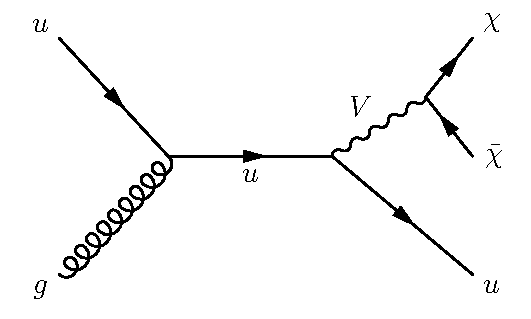
\includegraphics[width=\textwidth]{figures/monotop/diagrams/mj.pdf}
            \caption{$(g_{u}^{V,A})_{ij} \approx \delta_{ij}$}
            \label{fig:mt:fcncdiaga}
        \end{subfigure}
        \begin{subfigure}[t]{0.49\textwidth}
            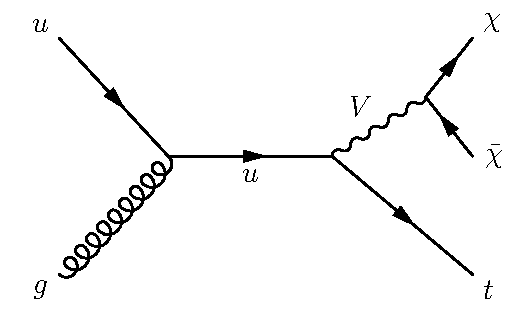
\includegraphics[width=\textwidth]{figures/monotop/diagrams/fcncb.pdf}
            \caption{$(g_{u}^{V,A})_{ij} \approx \delta_{i1}\delta_{j3} + \delta_{i3}\delta_{j1}$}
            \label{fig:mt:fcncdiagb}
        \end{subfigure}
        \caption{Possible DM production at the LHC, assuming a simplified spin-1 extension to the SM.}
        \label{fig:mt:fcncdiag}
    \end{center}
\end{figure}

In the second benchmark model, the charged, colored scalar $\phi$ couples to down-type quarks, or to a fermionic DM candidate $\psi$ and a top quark.
The interaction terms of the Lagrangian is given by:
\begin{equation}
    \mathcal{L}_\text{int} = \phi\overline{{d}}_i^C[(a_{q})^{ij}+(b_{q})^{ij}\gamma^5]{d}_j+\phi\overline{{t}}[a_{\psi}+b_{\psi}\gamma^5]\psi+\text{h.c.}
\end{equation}
There are 16 free parameters in this model, broadly organized in three categories:
\begin{itemize}
    \item The masses $m_\phi$ and $m_\psi$. (2)
    \item The couplings at the $\phi \bar{t} \psi$ vertex $a_\psi$ and $b_\psi$, which respectively control the strength of the scalar and pseudoscalar interactions. (2)
    \item The couplings at the $\phi \bar{d_i} d_j$ vertex $a_q^{ij}$ and $b_q^{ij}$ where $i,j=1,2,3$. Again, $a$ and $b$ refer the scalar and pseudoscalar couplings, respectively. (12)
\end{itemize}
In this model, mono-top production primarily occurs through the resonant decay of $\phi$ to $\psi$ and $t$, as shown in Figure~\ref{fig:mt:resdiag}.

\begin{figure}[]
    \begin{center}
        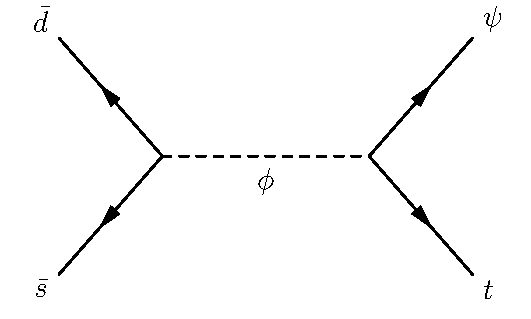
\includegraphics[width=0.5\textwidth]{figures/monotop/diagrams/resonant.pdf}
        \caption{Possible DM production at the LHC, assuming the existence of a charged, color scalar that couples to DM and the top quark.}
        \label{fig:mt:resdiag}
    \end{center}
\end{figure}

The two benchmark models show markedly different spectra in Figure~\ref{fig:mt:shapes}, motivating their use to test different modes of mono-top production.
The FCNC produces a falling \ptmiss~distribution, whereas the scalar resonance produces a \ptmiss~distribution peaking at approximately $m_\phi / 2$. 

\begin{figure}[]
    \begin{center}
        \begin{subfigure}[t]{0.49\textwidth}
            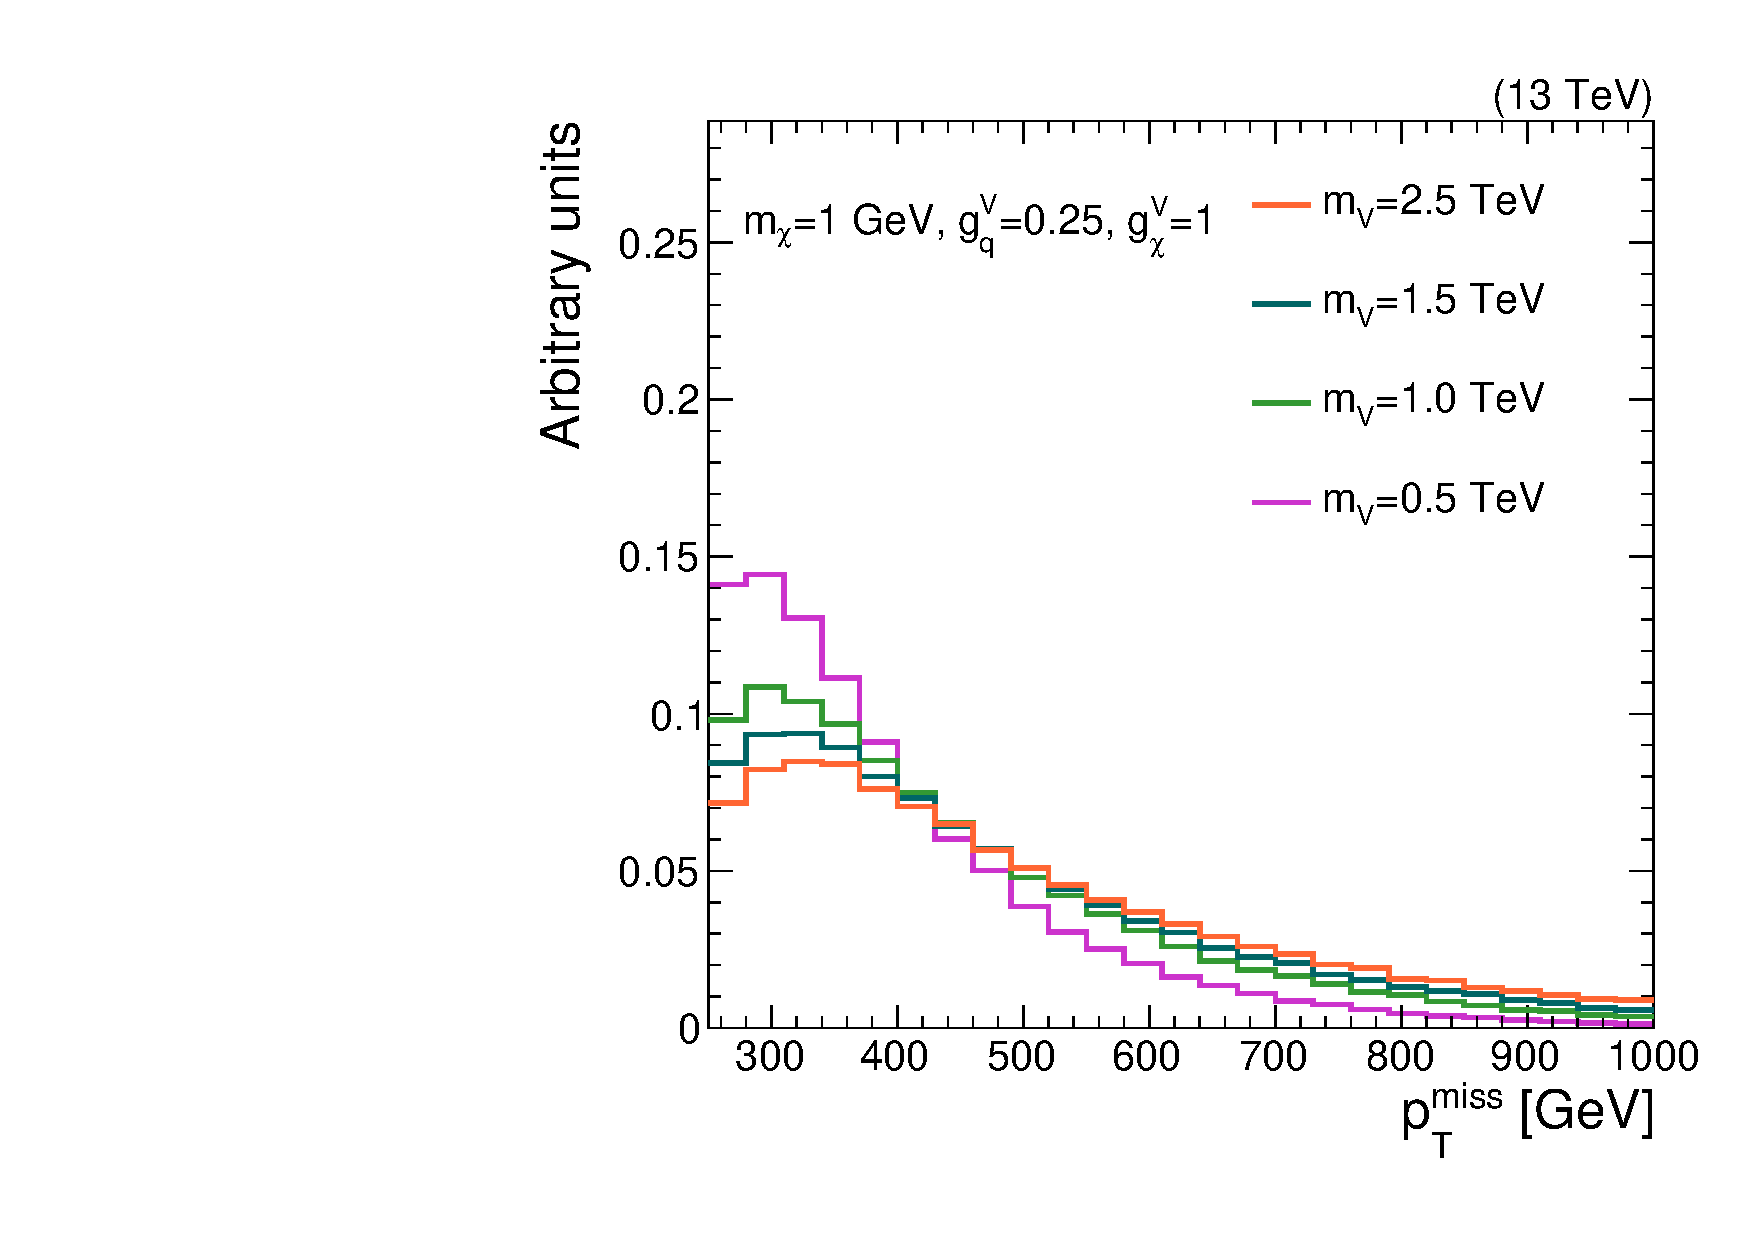
\includegraphics[width=\textwidth]{figures/monotop/diagrams/fcnc_pfmet.pdf}
            \caption{FCNC}
        \end{subfigure}
        \begin{subfigure}[t]{0.49\textwidth}
            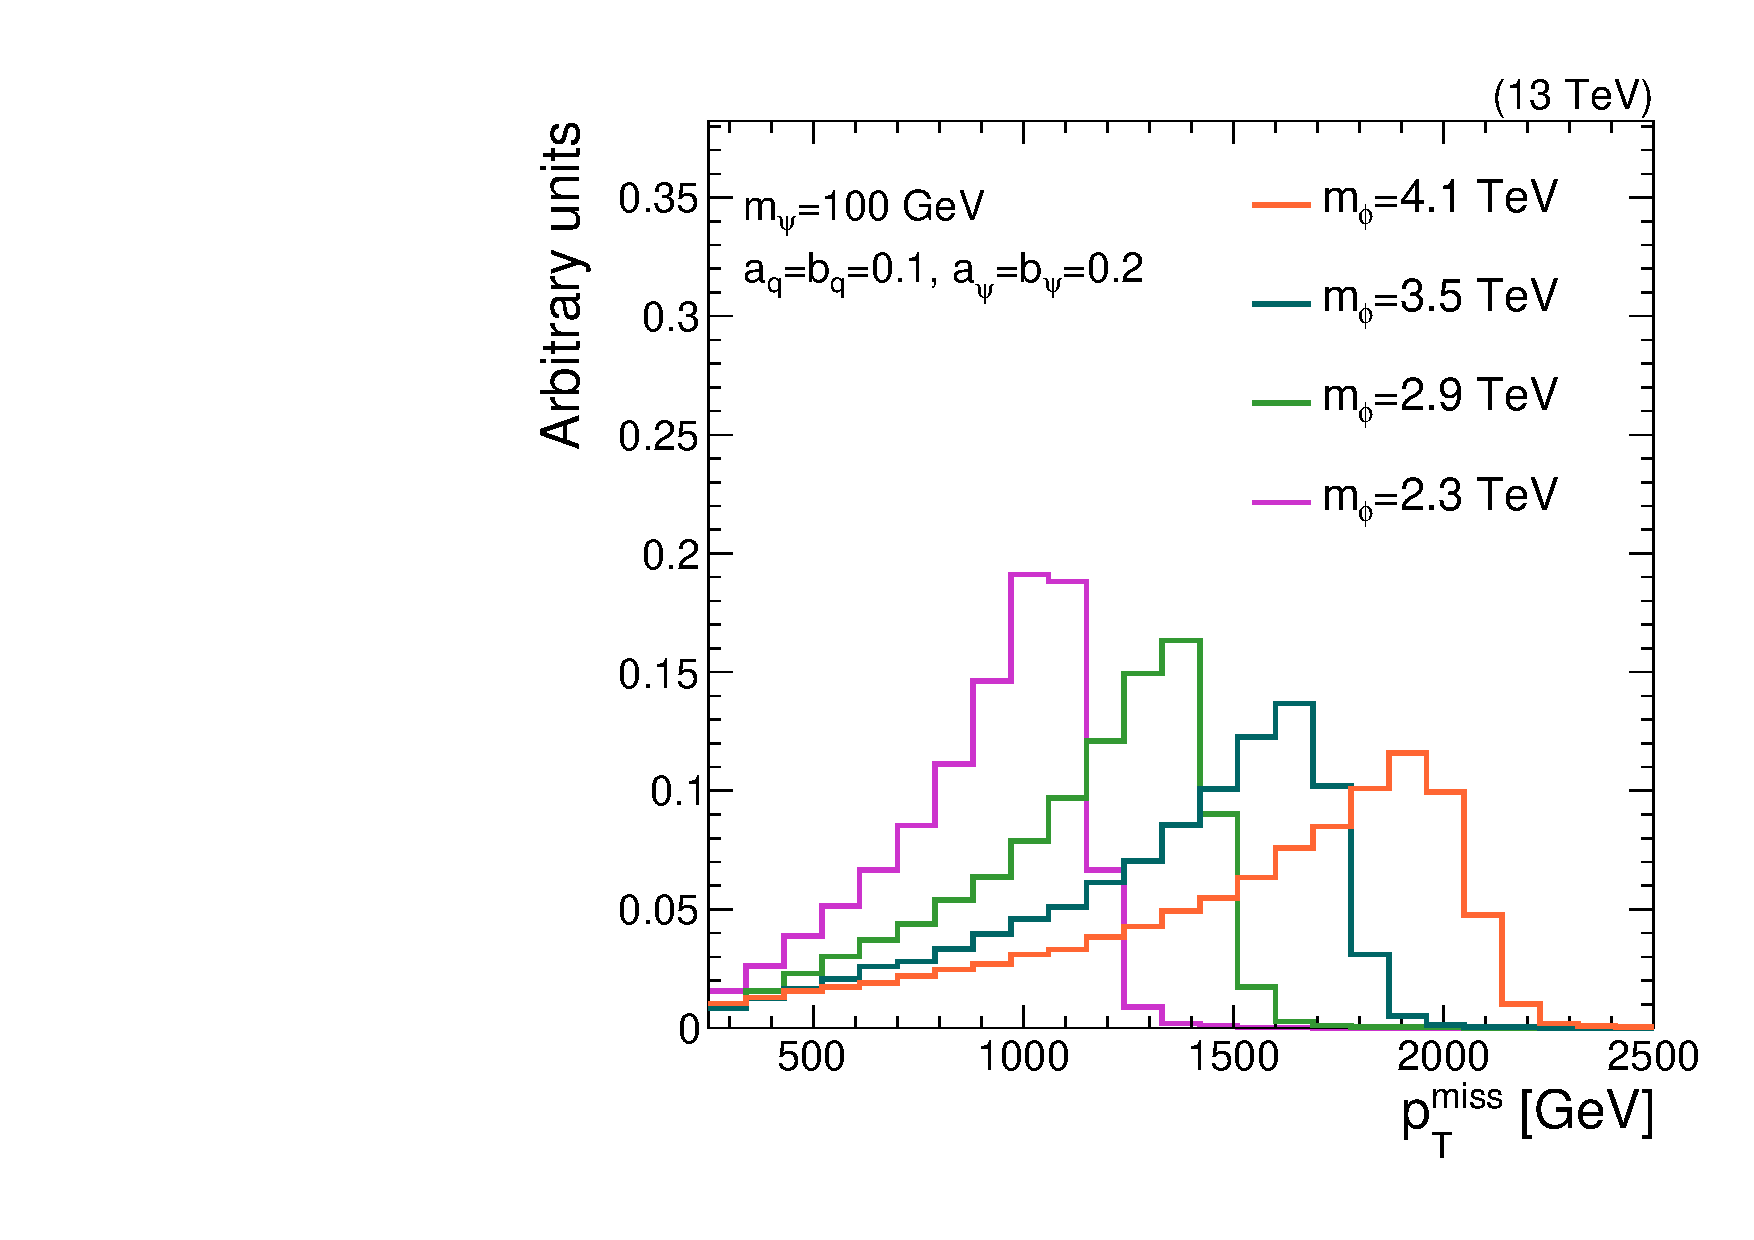
\includegraphics[width=\textwidth]{figures/monotop/diagrams/res_pfmet.pdf}
            \caption{Scalar resonance}
        \end{subfigure}
        \caption{Spectra of DM (missing) momentum under various signal hypothesis.}
        \label{fig:mt:shapes}
    \end{center}
\end{figure}

\clearpage

\section{Signal selection}
\label{sec:mt:sel}

When looking at events that pass a simple set of criteria (moderate $\ptmiss$ and one CA15 jet), it is clear (Figure~\ref{fig:mt:bkgshapes}) that the highest signal sensitivity is found in regions of high $\ptmiss$ and jet $\pt$.
The three primary background processes are:
\begin{itemize}
    \item $Z\rightarrow\nu\nu$. When the $Z$ is produced in association with one or more jets, the jet system can (with low probability) pass the criteria used to select a top jet. The neutrinos manifest as $\ptmiss$.
    \item $W\rightarrow\ell\nu$. As in the case of the $Z$, additional jets can mimic the signature of a top jet. Typically, the charged lepton in the final state is vetoed, but if it is out of acceptance ($e,\mu$) or fails ID criteria ($\tau_\mathrm{h}$), then it is not identified. 
    \item $t\bar{t} \rightarrow bq\bar{q}' + \bar{b}\ell\nu$. As in the case of the $W$, a charged lepton in the final state may not be properly identified. Unlike the previous two processes, a semi-leptonic $t\bar{t}$ event contains a real hadronic top quark decay. 
\end{itemize}

\begin{figure}[]
    \begin{center}
        \begin{subfigure}[t]{0.49\textwidth}
            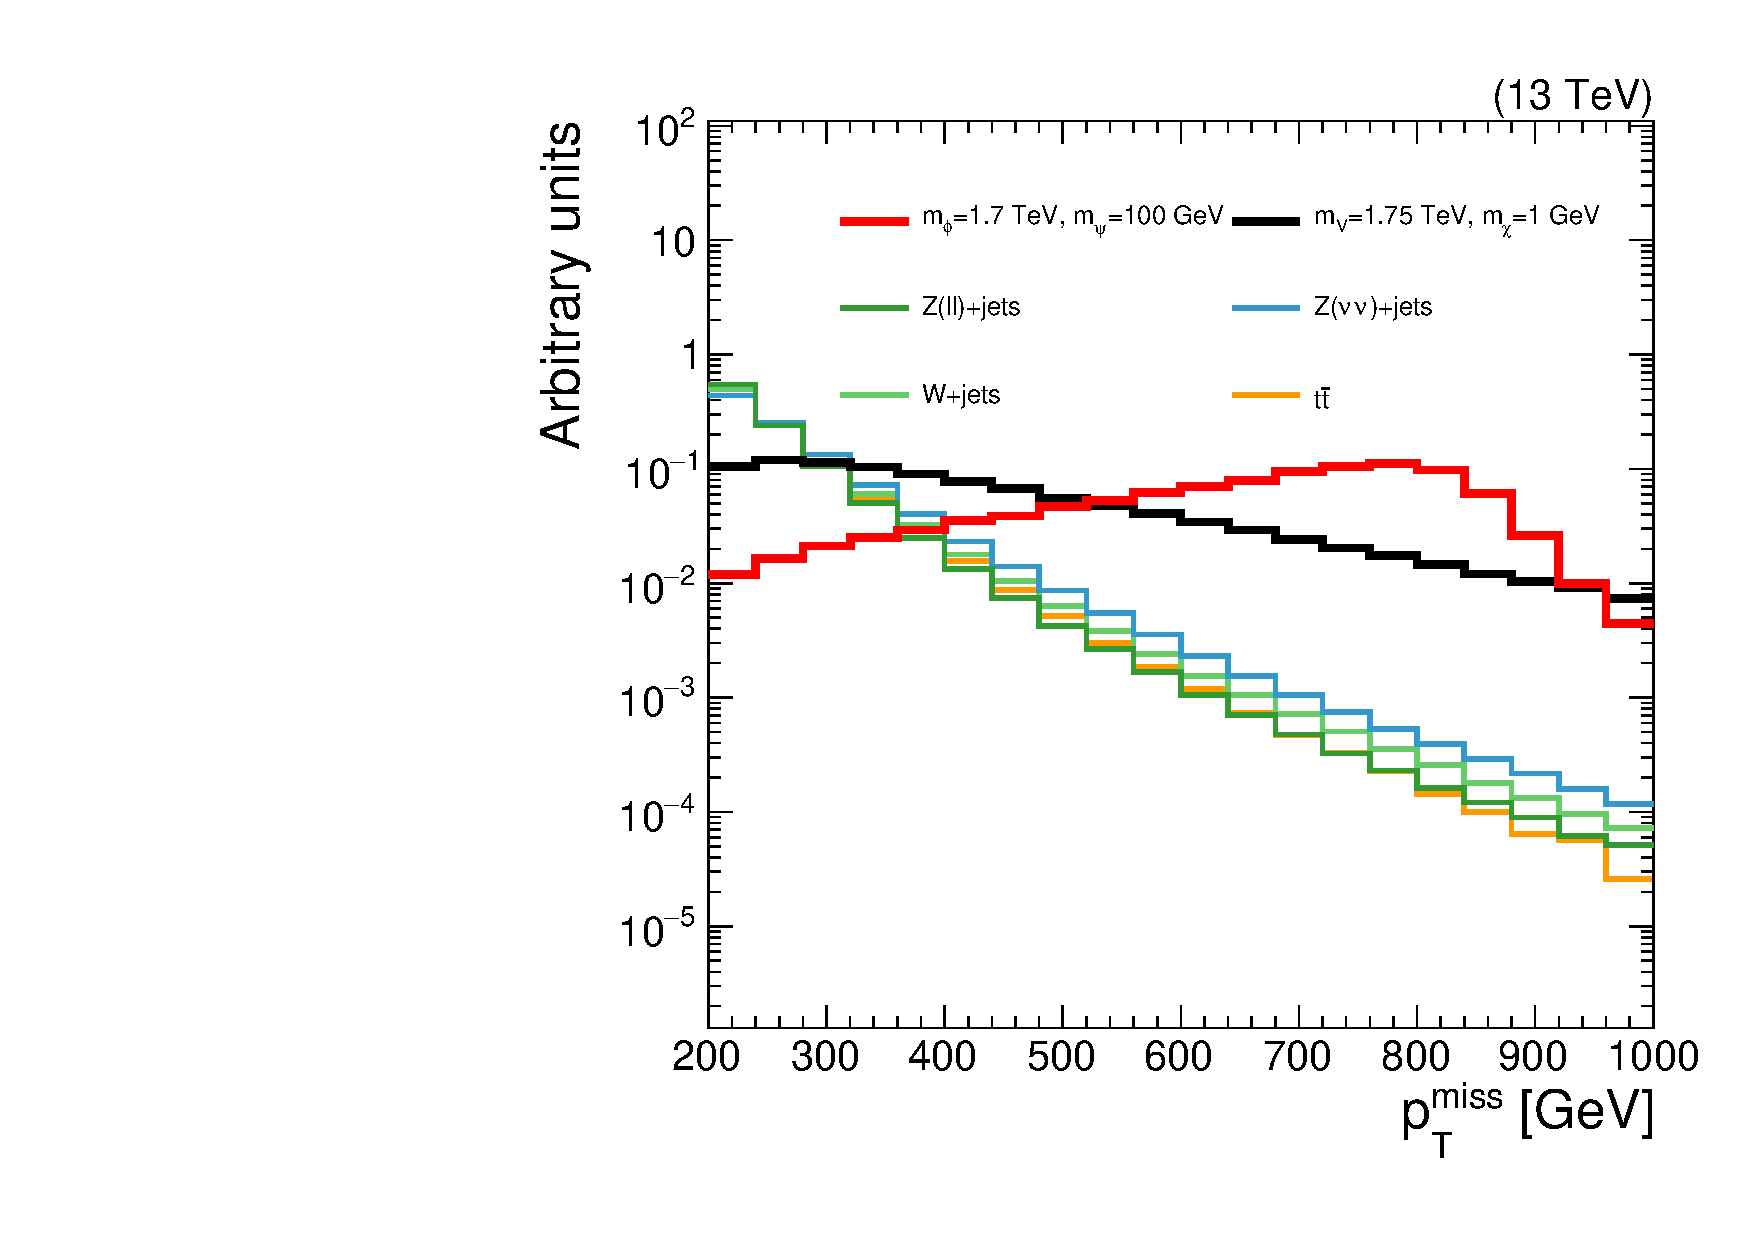
\includegraphics[width=\textwidth]{figures/monotop/shapes/signal_pfmet_logy.pdf}
            \caption{Missing momentum}
        \end{subfigure}
        \begin{subfigure}[t]{0.49\textwidth}
            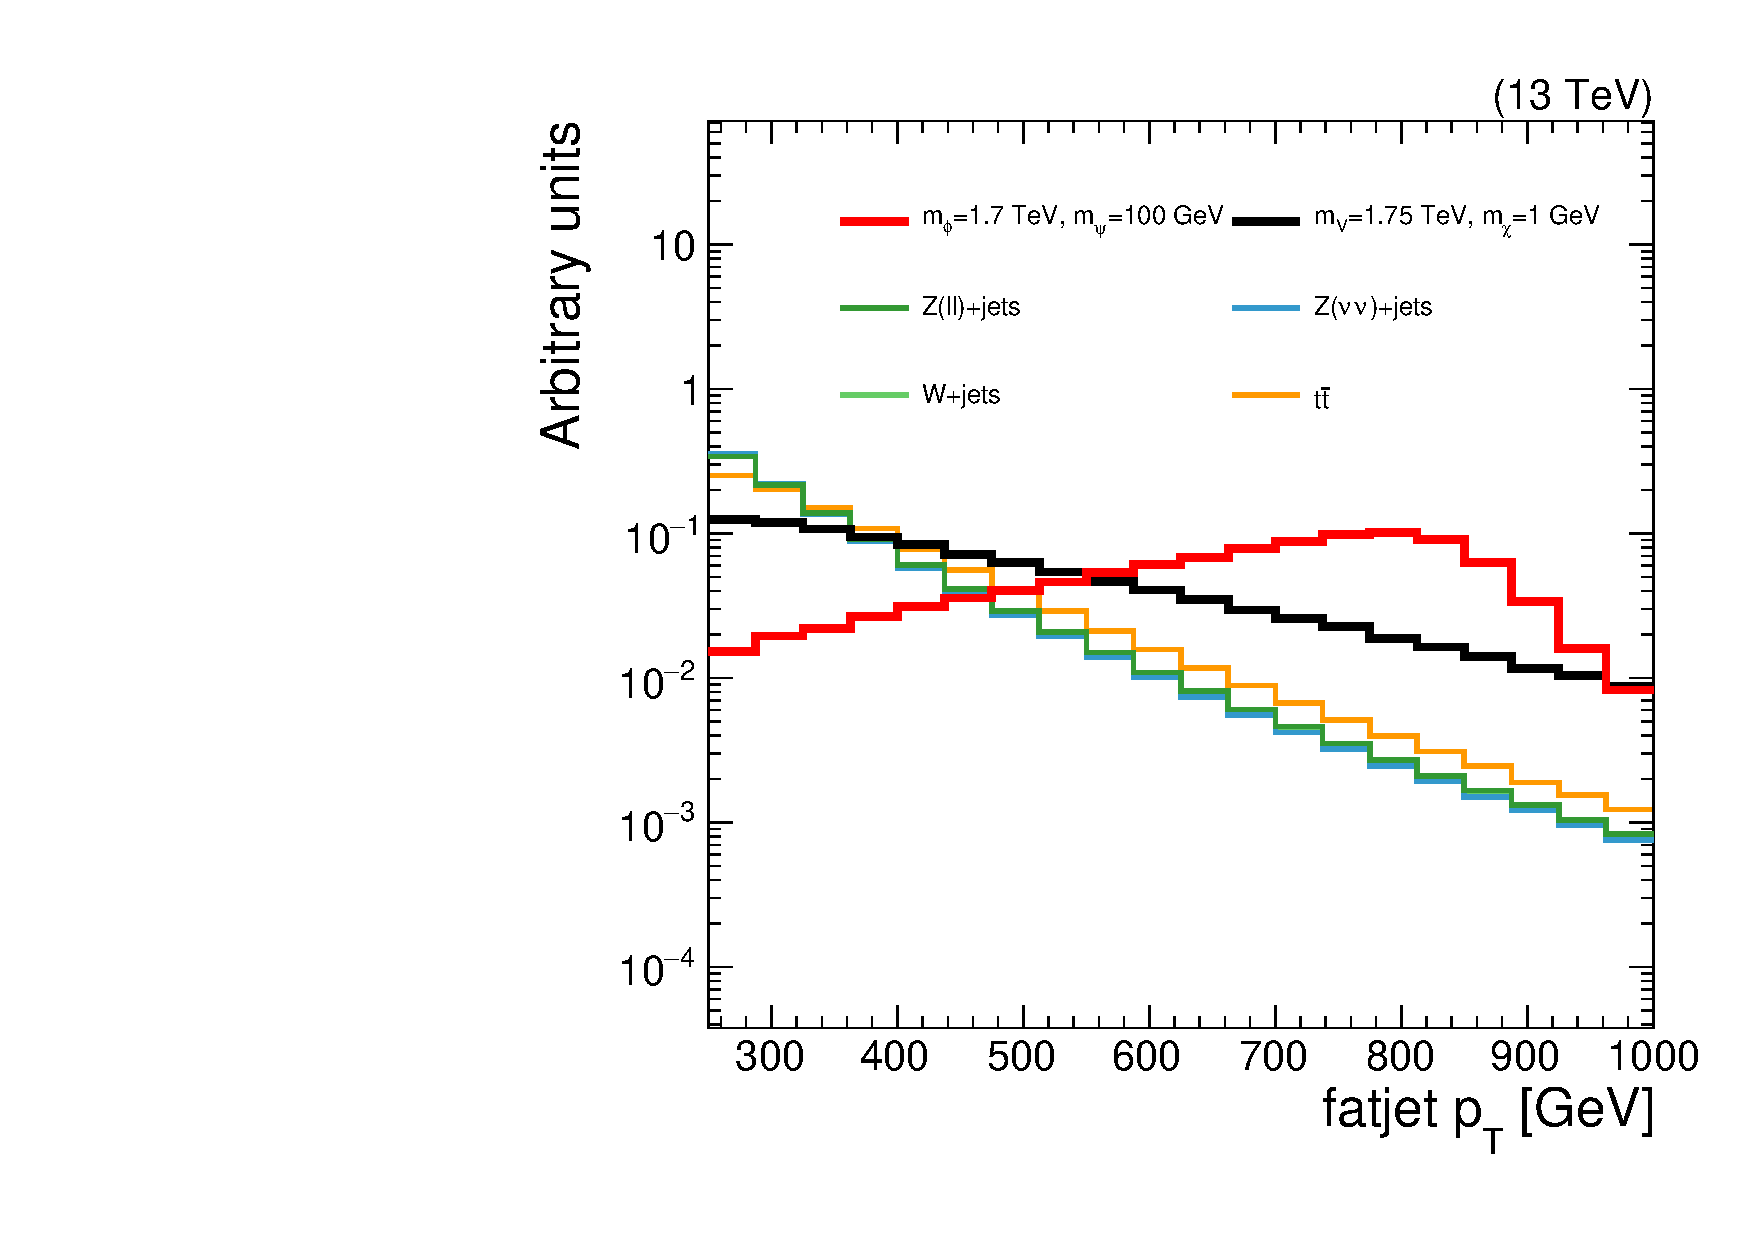
\includegraphics[width=\textwidth]{figures/monotop/shapes/signal_fjPt_0__logy.pdf}
            \caption{Jet $\pt$}
        \end{subfigure}
        \caption{Comparison of missing and jet momenta in various backgrounds and signal models.}
        \label{fig:mt:bkgshapes}
    \end{center}
\end{figure}

Events in the signal regions (SRs) are then selected according to Table~\ref{tab:mt:cuts}, chosen to be consistent with the signal topology while mitigating the aforementioned SM backgrounds.
As described in Section~\ref{sec:jets:combined}, two working points (WPs) are defined for the top ID BDT.
The signal events (passing all other selection criteria) are partitioned into a ``loose'' SR and a ``tight'' SR on the basis of which WP the top candidate jet satisfies. 

\begin{table}[]
    \caption{Criteria used to select events for the mono-top search signal regions. Note that two SRs are defined, based on the BDT score.}
    \label{tab:mt:cuts}
    \begin{tabular}{p{0.4\textwidth}p{0.6\textwidth}}
        Criterion & Notes \\ 
        \hline 
        \hline 
        $\ptmiss>250$ GeV & Signal events should have large missing momentum. Exact threshold is chosen to maximize online trigger efficiency. \\ 
        1 CA15 jet with $\pt>250$ GeV & Top quark candidate. Recoils against $\ptmiss$, so threshold is set at $250$ GeV. \\ 
        CA15 jet $110 < m_\mathrm{SD} < 210$ GeV & Consistency with top quark mass. \\ 
        At least one $b$-tagged sub-jet & Identifying $B$ hadron produced from top decay/hadronization. \\ 
        No $b$-tagged narrow jets & Rejecting semi-leptonic $t\bar{t}$ decays. \\ 
        \hline 
        No identified $e,\mu,\tau_\mathrm{h}$ & Suppress $W$+jet and $t\bar{t}$ processes. \\ 
        No identified $\gamma$ & Suppress $\gamma$+jet processes. \\ 
        \hline 
        $\min_\mathrm{jets}\Delta\phi(\mathrm{jet},\ptmiss) > 0.5$ & Remove events with large $\ptmiss$ caused by mismeasured jets. \\ 
        \hline 
        CA15 jet BDT & Identifying top decay structure. If the jet passes the tight WP, it is placed in the ``tight'' SR. Otherwise, if it only passes the loose WP, it is placed in the ``loose'' SR.\\ 
    \end{tabular}
\end{table}

Figure~\ref{fig:mt:prefit_signal} shows the $\ptmiss$ distributions, as predicted by MC and as observed in collected data, in the two signal regions.

\begin{figure}[]
    \begin{center}
        \begin{subfigure}[t]{0.49\textwidth}
            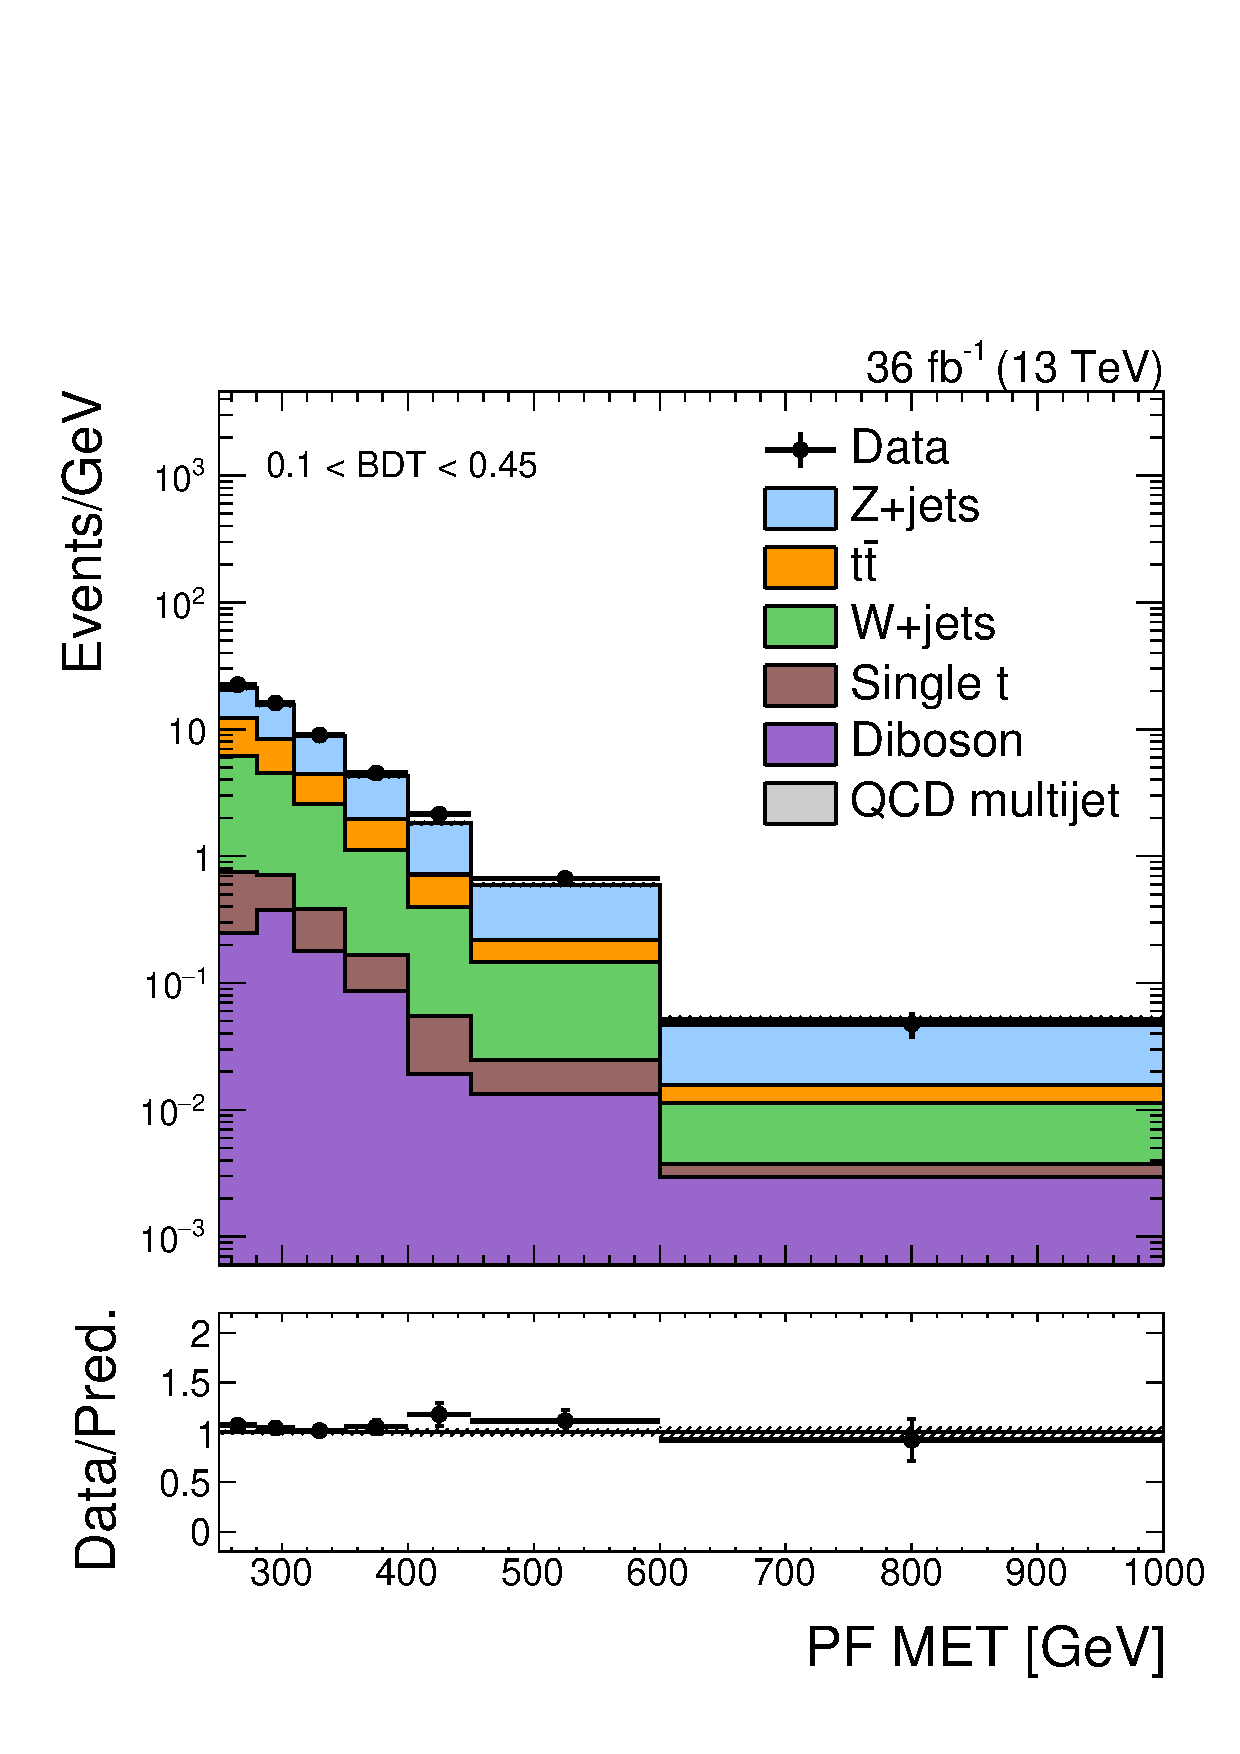
\includegraphics[width=\textwidth]{figures/monotop/prefit/signal_loose_pfmet_logy.pdf}
            \caption{Loose SR}
        \end{subfigure}
        \begin{subfigure}[t]{0.49\textwidth}
            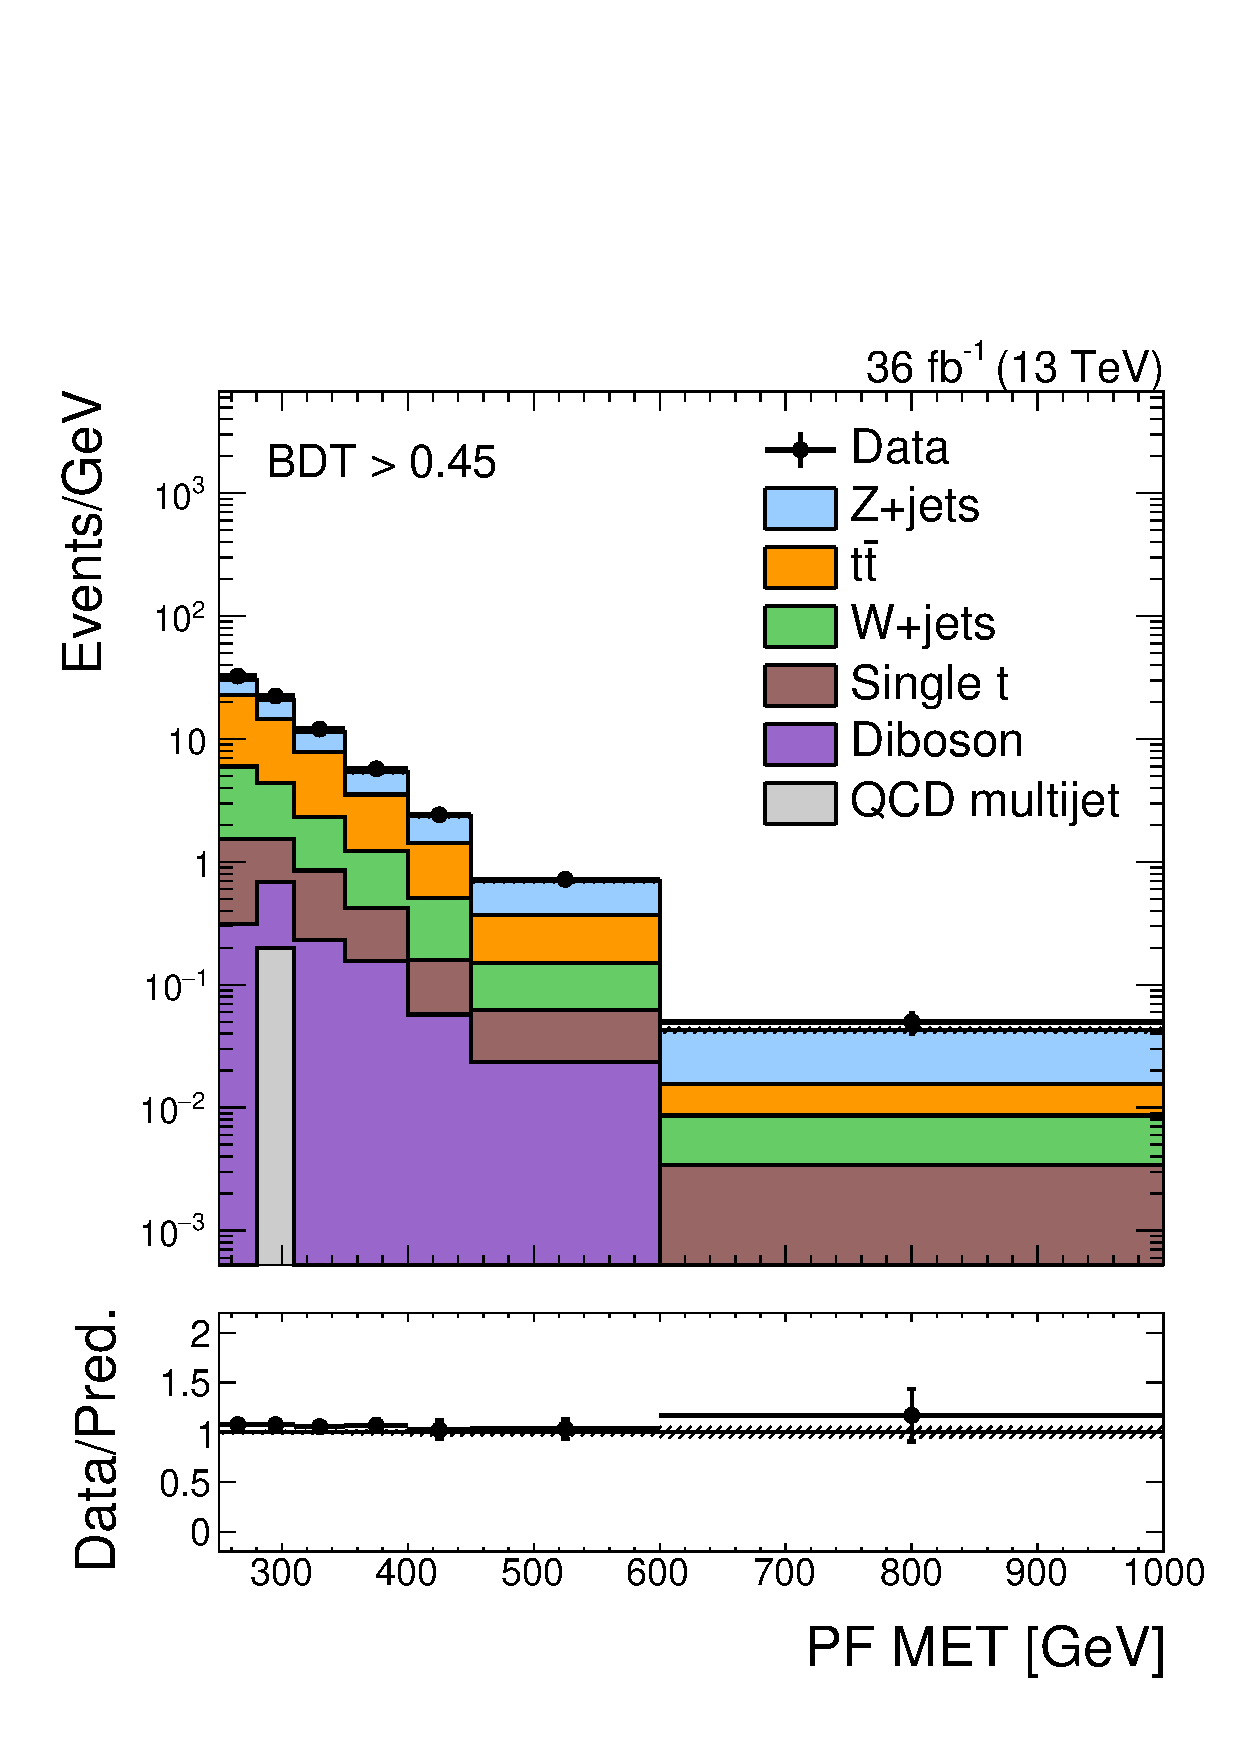
\includegraphics[width=\textwidth]{figures/monotop/prefit/signal_tight_pfmet_logy.pdf}
            \caption{Tight SR}
        \end{subfigure}
        \caption{$\ptmiss$ distributions in the two mono-top signal regions.
                 The bottom section of each figure shows the ratio of the data and the prediction.
                 The only uncertainties plotted in these figures are those arising from Poisson fluctations in data (black bars) and MC (grey band).}
        \label{fig:mt:prefit_signal}
    \end{center}
\end{figure}

\clearpage

\section{Background estimation}
\label{sec:mt:bkg}

Searching for DM amounts to looking for an excess of data events over the SM prediction at large values of $\ptmiss$.
Therefore, the $\ptmiss$ distribution of the three primary SM backgrounds described in Section~\ref{sec:mt:sel} must be predicted with small uncertainty.
The MC simulation provides a reasonable description of the data, but the theoretical uncertainties inherent in the MC (primarily due to higher-order QCD effects) can range up to $20\%$.
To reduce the prediction uncertainty further, a ``data-driven'' approach is used to estimate the SM processes in the SR.
In this context, ``data-driven'' refers to the use of control data (i.e. data that cannot contain signal) to directly estimate or supplement the estimation of SM processes in the SR.

\subsection{Visible final states to constrain invisible final states}

As a starting point, let us tackle the estimation of $Z\rightarrow\nu\nu$ in the SR.
Since the momentum imbalance (up to experimental effects) in a $Z\rightarrow\nu\nu$ event is just the transverse momentum of the $Z$ boson ($\pt^Z$), we must estimate $\pt^Z$.
To good approximation, the $\pt^Z$ distribution is independent of the decay mode of the $Z$ boson.
Therefore, it is natural to estimate $\ptmiss(Z\rightarrow\nu\nu)$ by measuring $\pt^Z(Z\rightarrow\mu\mu)$, as muons are easily identifiable and reconstructible. 

However, there is one important distinction between $\nu\nu$ and $\mu\mu$ events.
In the latter, $\pt^Z$ can be directly measured, whereas in the former it must be inferred through a momentum imbalance.
Effects like jet energy scale and acceptance can impact $\ptmiss$, but not $\pt^{\mu\mu}$. 
Therefore, instead of directly measuring $\pt^{\mu\mu}$ in $\mu\mu$ events, we define and use the hadronic recoil $U$:
\begin{equation}
    \vec{U} = \vptmiss + \sum_{\mu} \vpt^{~\mu} + \sum_{e} \vpt^{~e} + \sum_\gamma \vpt^{~\gamma}
\end{equation}
In the SR (where there are no $e,\mu,\gamma$), $U = \ptmiss$.
In $Z\rightarrow\mu\mu$ events, $U$ mimics the momentum imbalance, if we had pretended the identified muons did not exist when computing $\ptmiss$. 
Therefore, $U$ is an exact analogy for $\ptmiss$ in the SR.
Figure~\ref{fig:mt:zvsz} makes the same argument in a schematic fashion. 

\begin{figure}[]
    \begin{center}
        \begin{subfigure}[t]{0.49\textwidth}
            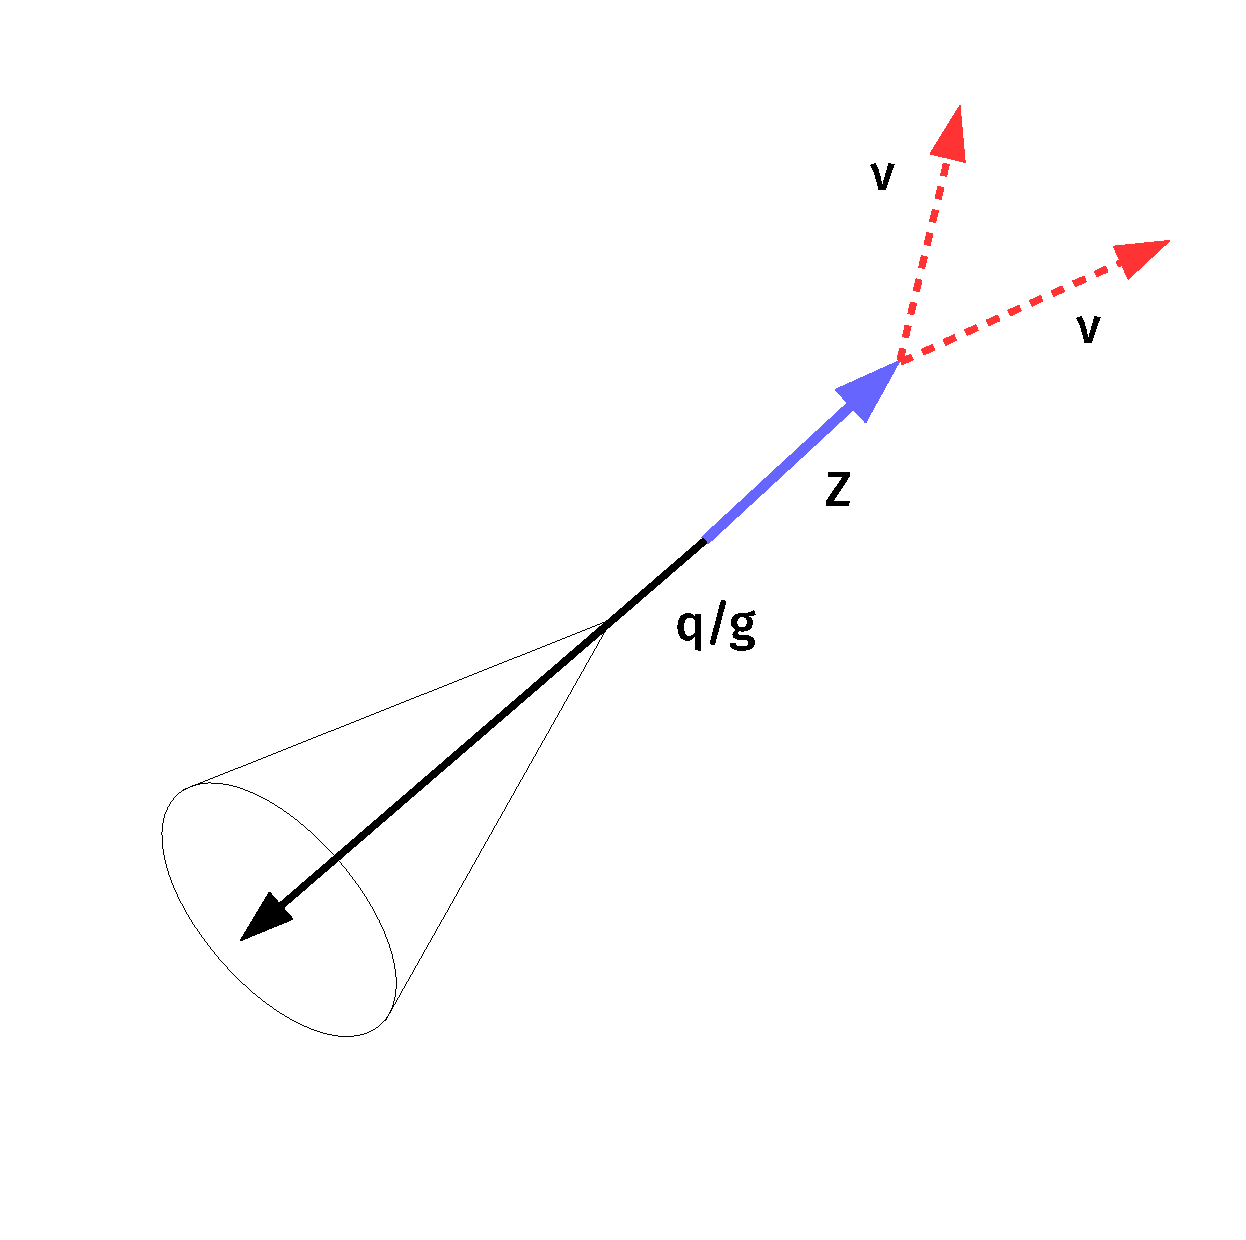
\includegraphics[width=\textwidth]{figures/monotop/diagrams/zsr.pdf}
            \caption{$Z\rightarrow\nu\nu$}
        \end{subfigure}
        \begin{subfigure}[t]{0.49\textwidth}
            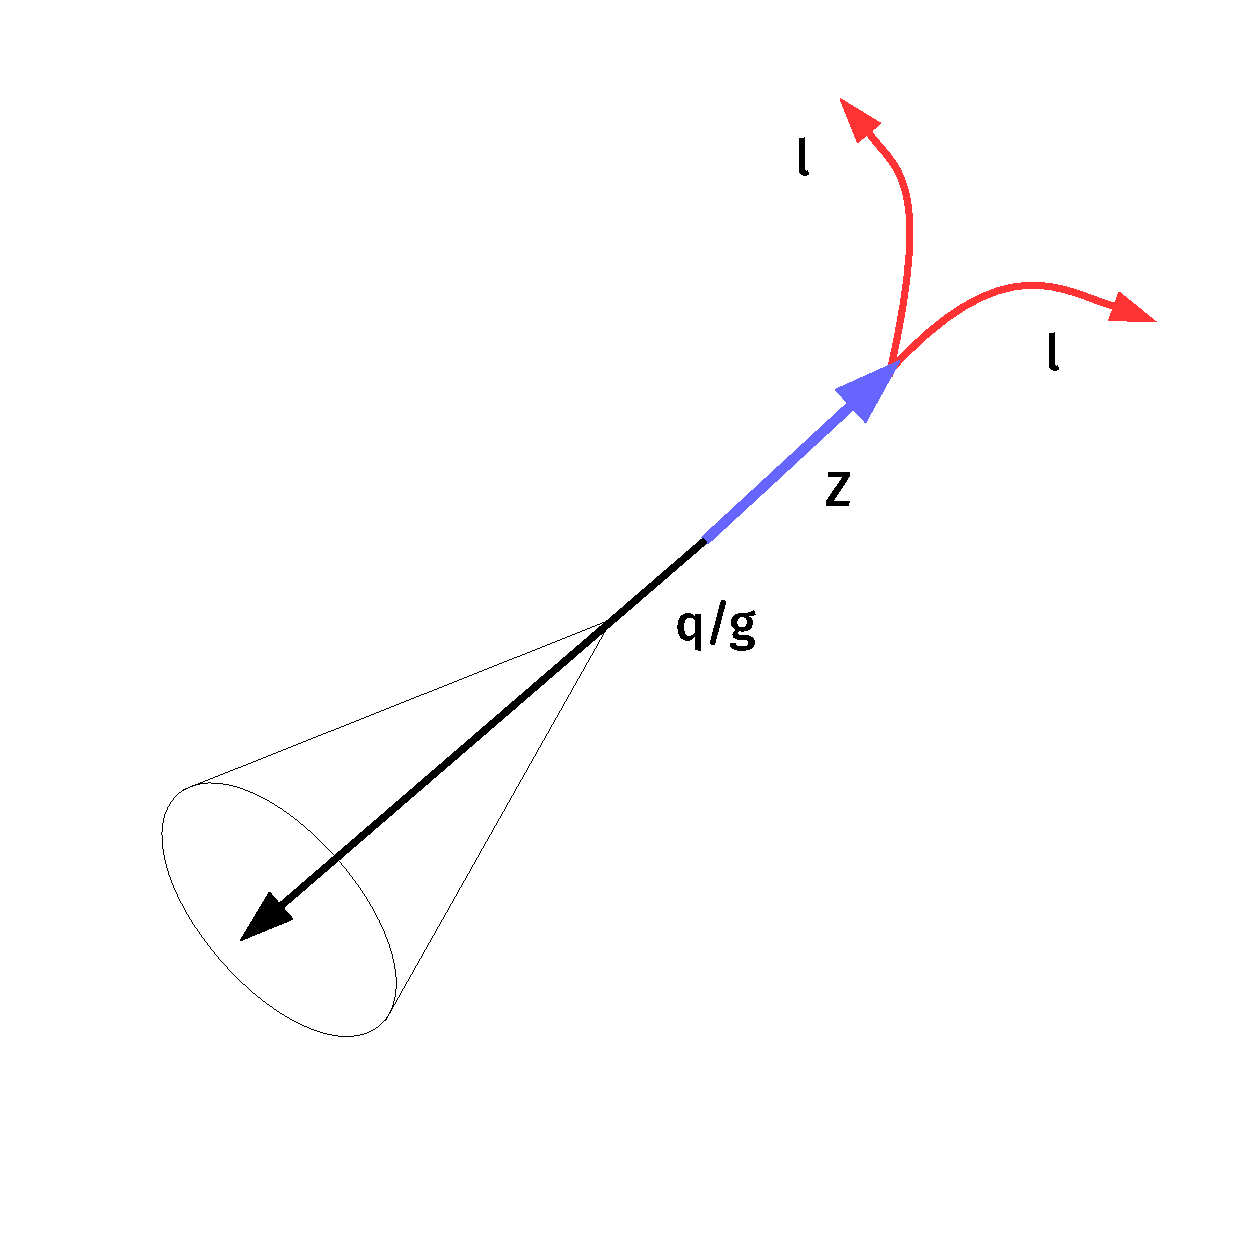
\includegraphics[width=\textwidth]{figures/monotop/diagrams/zcr.pdf}
            \caption{$Z\rightarrow\mu\mu$}
        \end{subfigure}
        \caption{Schematic representation of two $Z$ decay modes: to neutrinos (as in the SR) and to muons (as in the CRs).
                 Note that in both cases, $U$ is sensitive to the same effects arising from the measurement of the jet recoiling against the $Z$ boson, whereas $\pt^{\mu\mu}$ is largely independent of the jet.}
        \label{fig:mt:zvsz}
    \end{center}
\end{figure}

Table~\ref{tab:mt:zmm_cuts} describes the criteria used to define events in the ``$\mu\mu$'' control regions (CRs). 
Figure~\ref{fig:mt:prefit_dimuon} shows the distribution of $U$ in these CRs, as well as the $m_{\mu\mu}$ and $\pt^\mu$ distributions. 

\begin{table}[]
    \caption{Criteria used to select events for the mono-top $Z\rightarrow\mu\mu$ CR. As with the SR, the region is further split based on the jet BDT score.}
    \label{tab:mt:zmm_cuts}
    \centering
    \begin{tabular}{p{0.4\textwidth}p{0.6\textwidth}}
        Criterion & Notes \\ 
        \hline 
        \hline 
        $U>250$ GeV & Mimicking the selection in the SR; also constrained by trigger thresholds. \\ 
        1 CA15 jet with $\pt>250$ GeV &  Same as SR \\ 
        CA15 jet $110 < m_\mathrm{SD} < 210$ GeV & Same as SR \\ 
        \hline 
        Well-identified $\mu^-,\mu^+$ pair, with $|m_{\mu\mu}-m_Z|<30$ GeV & Identifying the $Z\rightarrow\mu\mu$ resonance. \\ 
        No identified $e,\tau_\mathrm{h}$ & Same as SR. \\ 
        No identified $\gamma$ & Same as SR \\ 
        \hline 
        $\min_\mathrm{jets}\Delta\phi(\mathrm{jet},U) > 0.5$ & Same as SR \\ 
        \hline 
        CA15 jet BDT & Same as SR\\ 
    \end{tabular}
\end{table}

\begin{figure}[]
    \begin{center}
        \begin{subfigure}[t]{0.49\textwidth}
            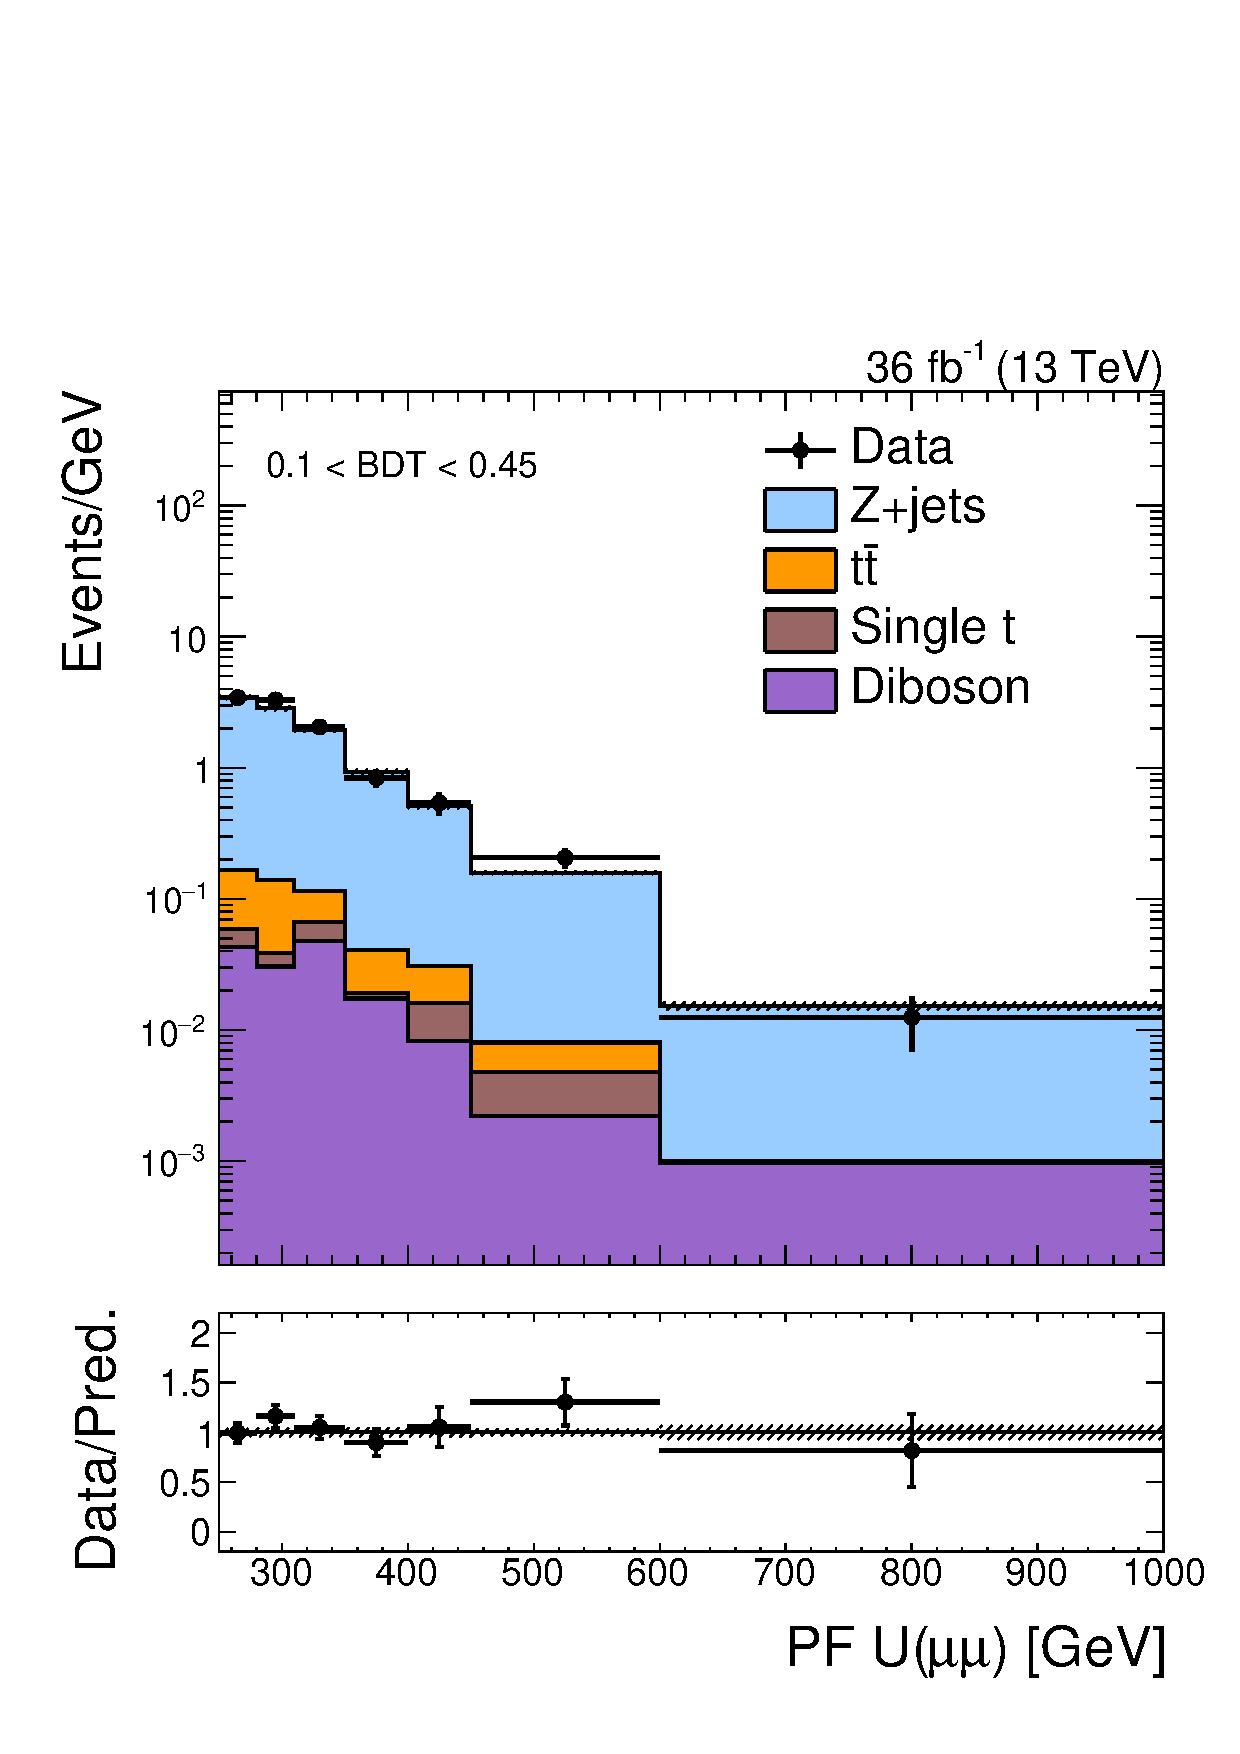
\includegraphics[width=\textwidth]{figures/monotop/prefit/dimuon_loose_pfUZmag_logy.pdf}
            \caption{$U$ in loose CR}
        \end{subfigure}
        \begin{subfigure}[t]{0.49\textwidth}
            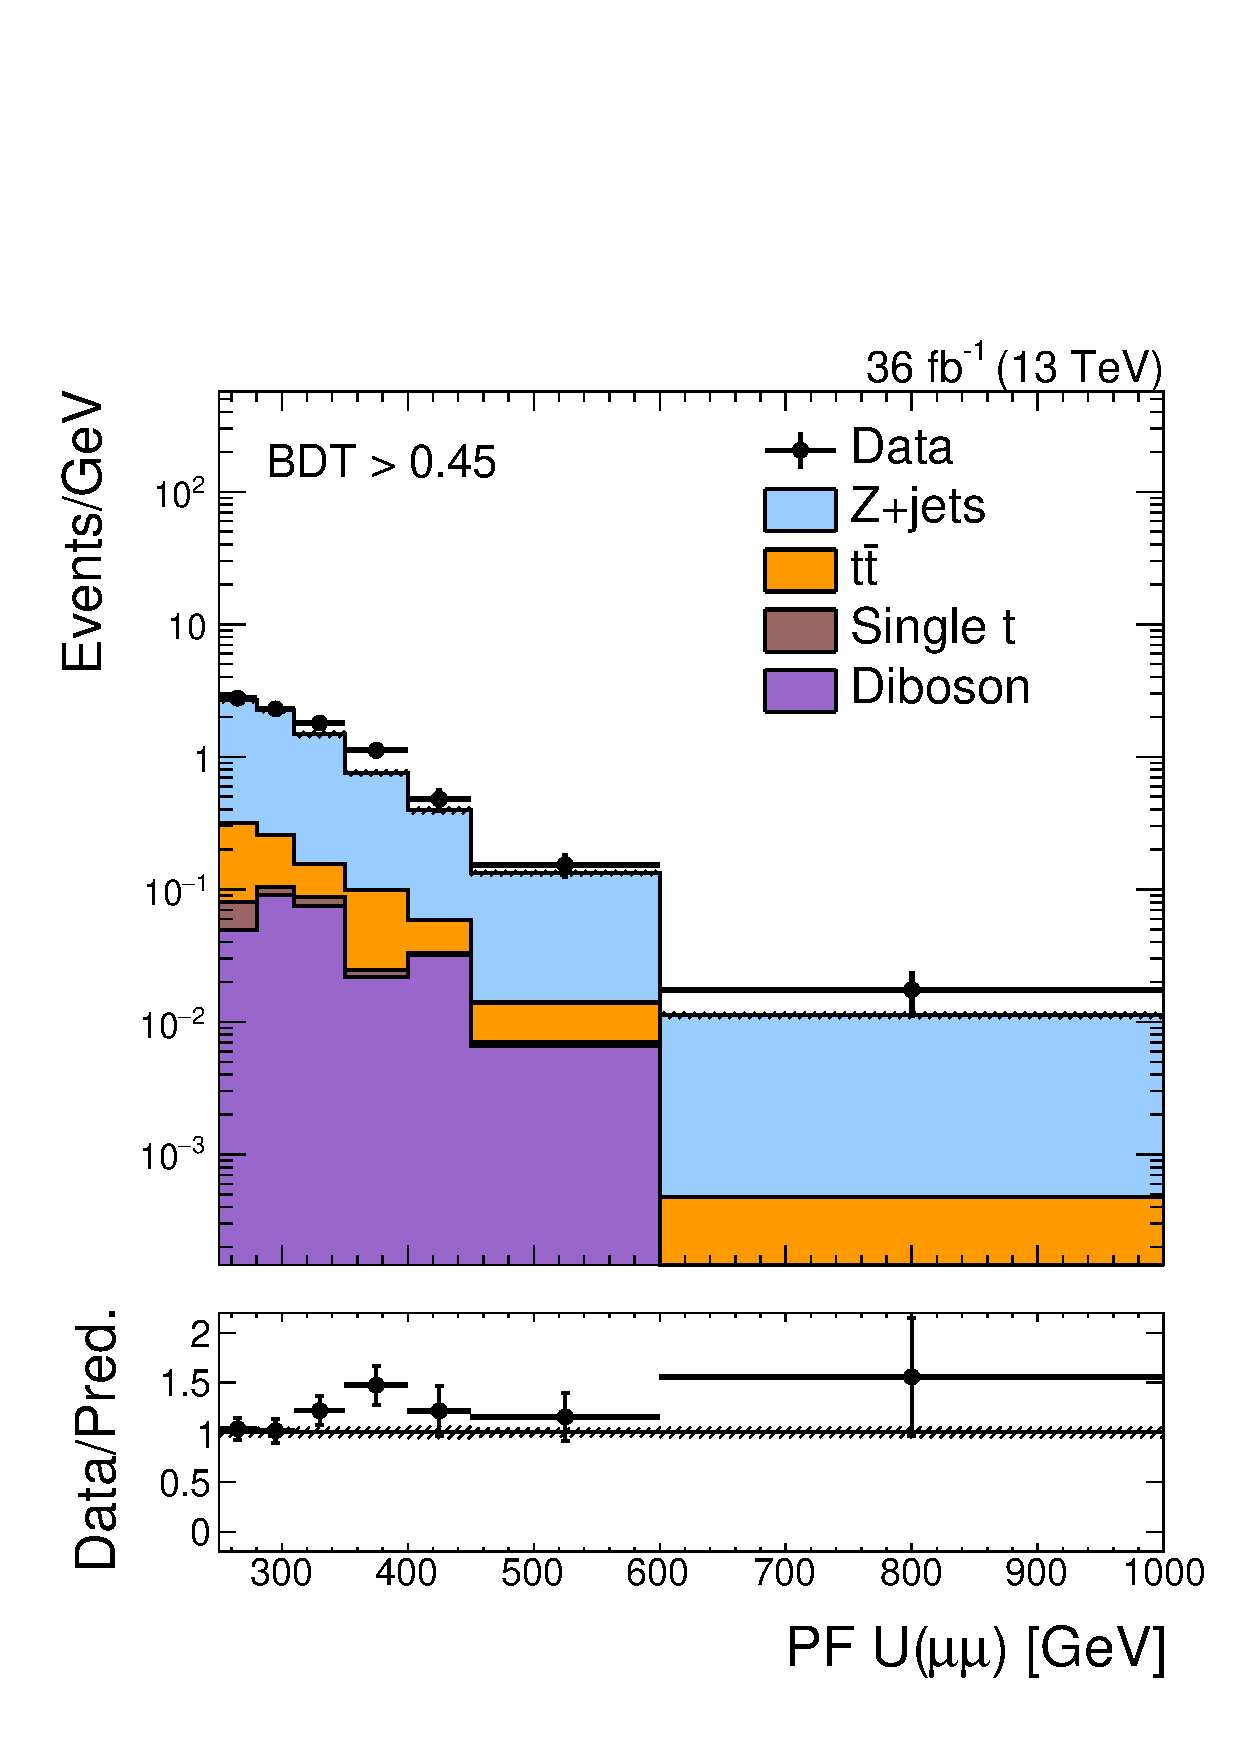
\includegraphics[width=\textwidth]{figures/monotop/prefit/dimuon_tight_pfUZmag_logy.pdf}
            \caption{$U$ in tight CR}
        \end{subfigure}
        \begin{subfigure}[t]{0.49\textwidth}
            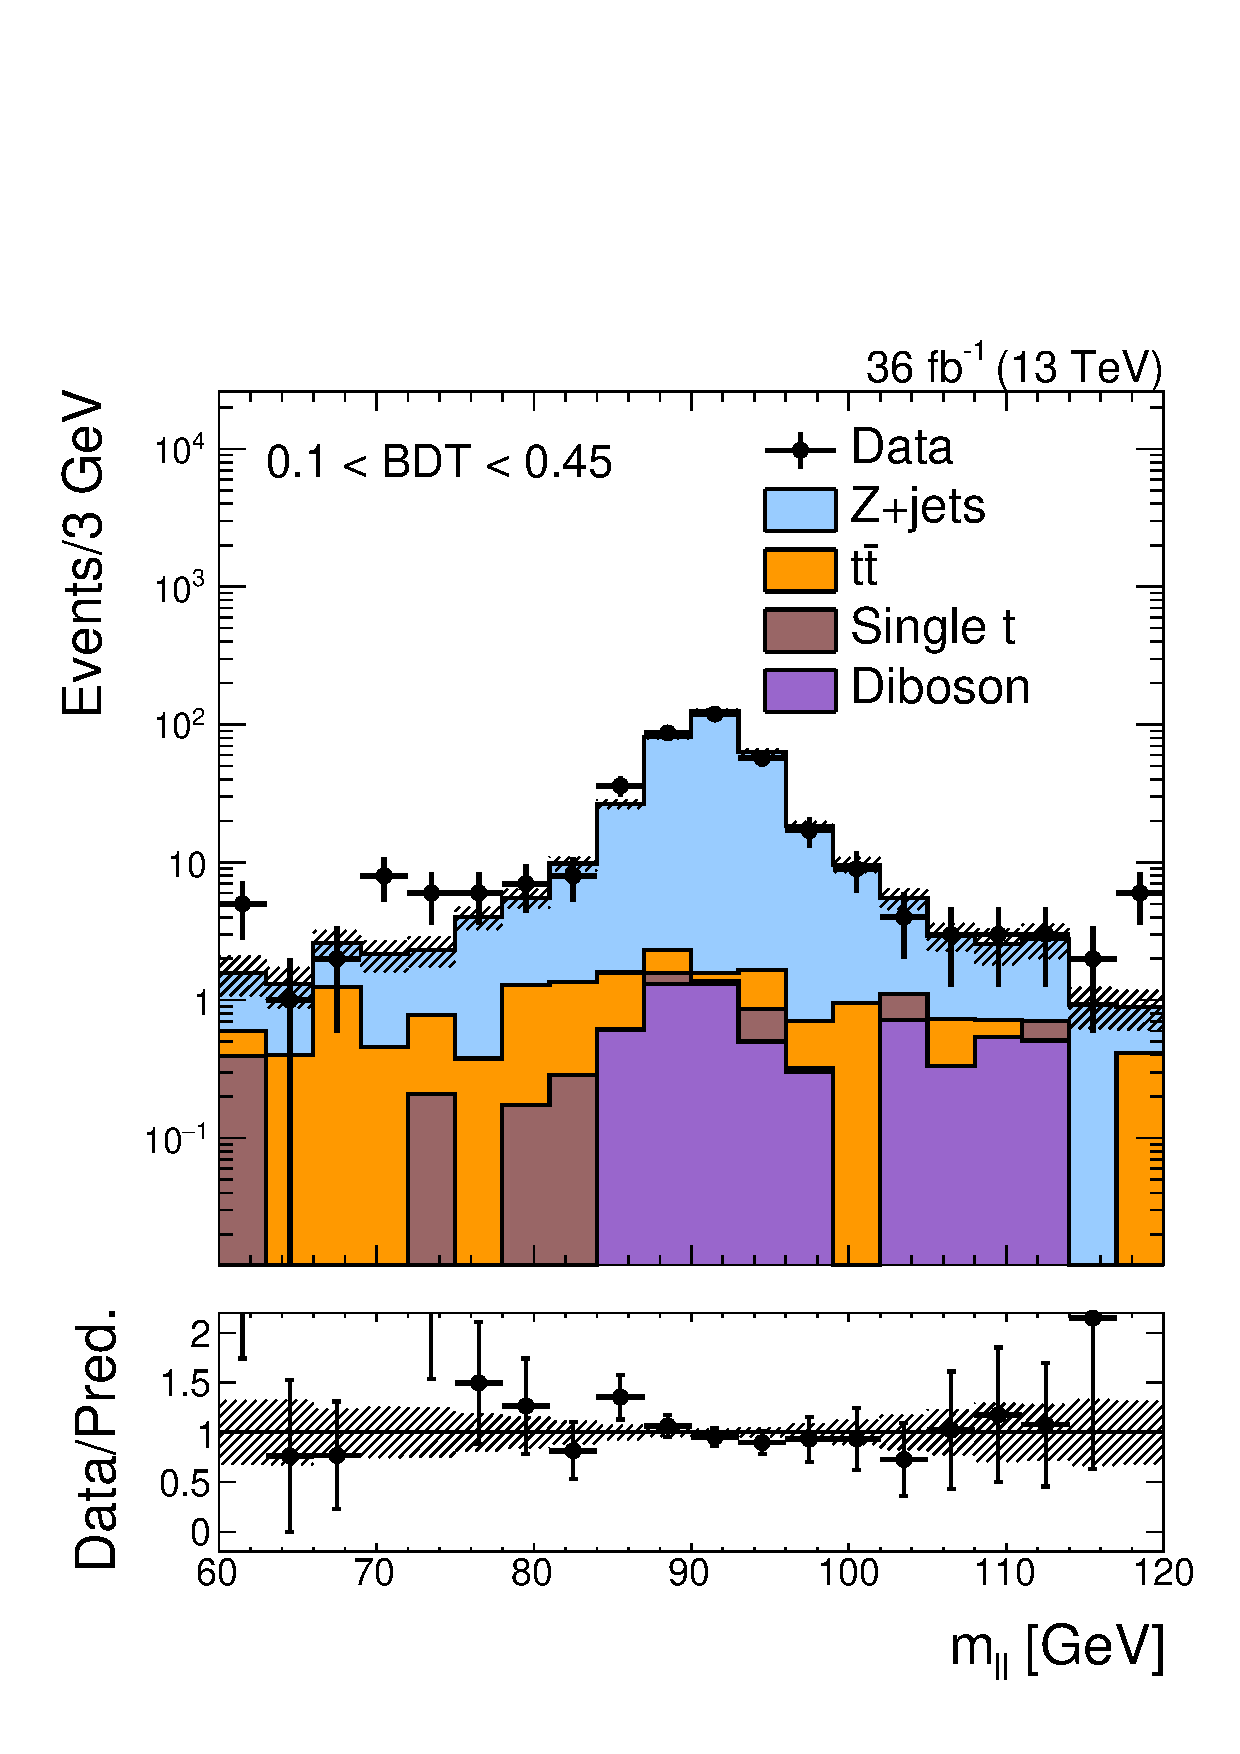
\includegraphics[width=\textwidth]{figures/monotop/prefit/dimuon_loose_diLepMass_logy.pdf}
            \caption{$m_{\mu\mu}$}
        \end{subfigure}
        \begin{subfigure}[t]{0.49\textwidth}
            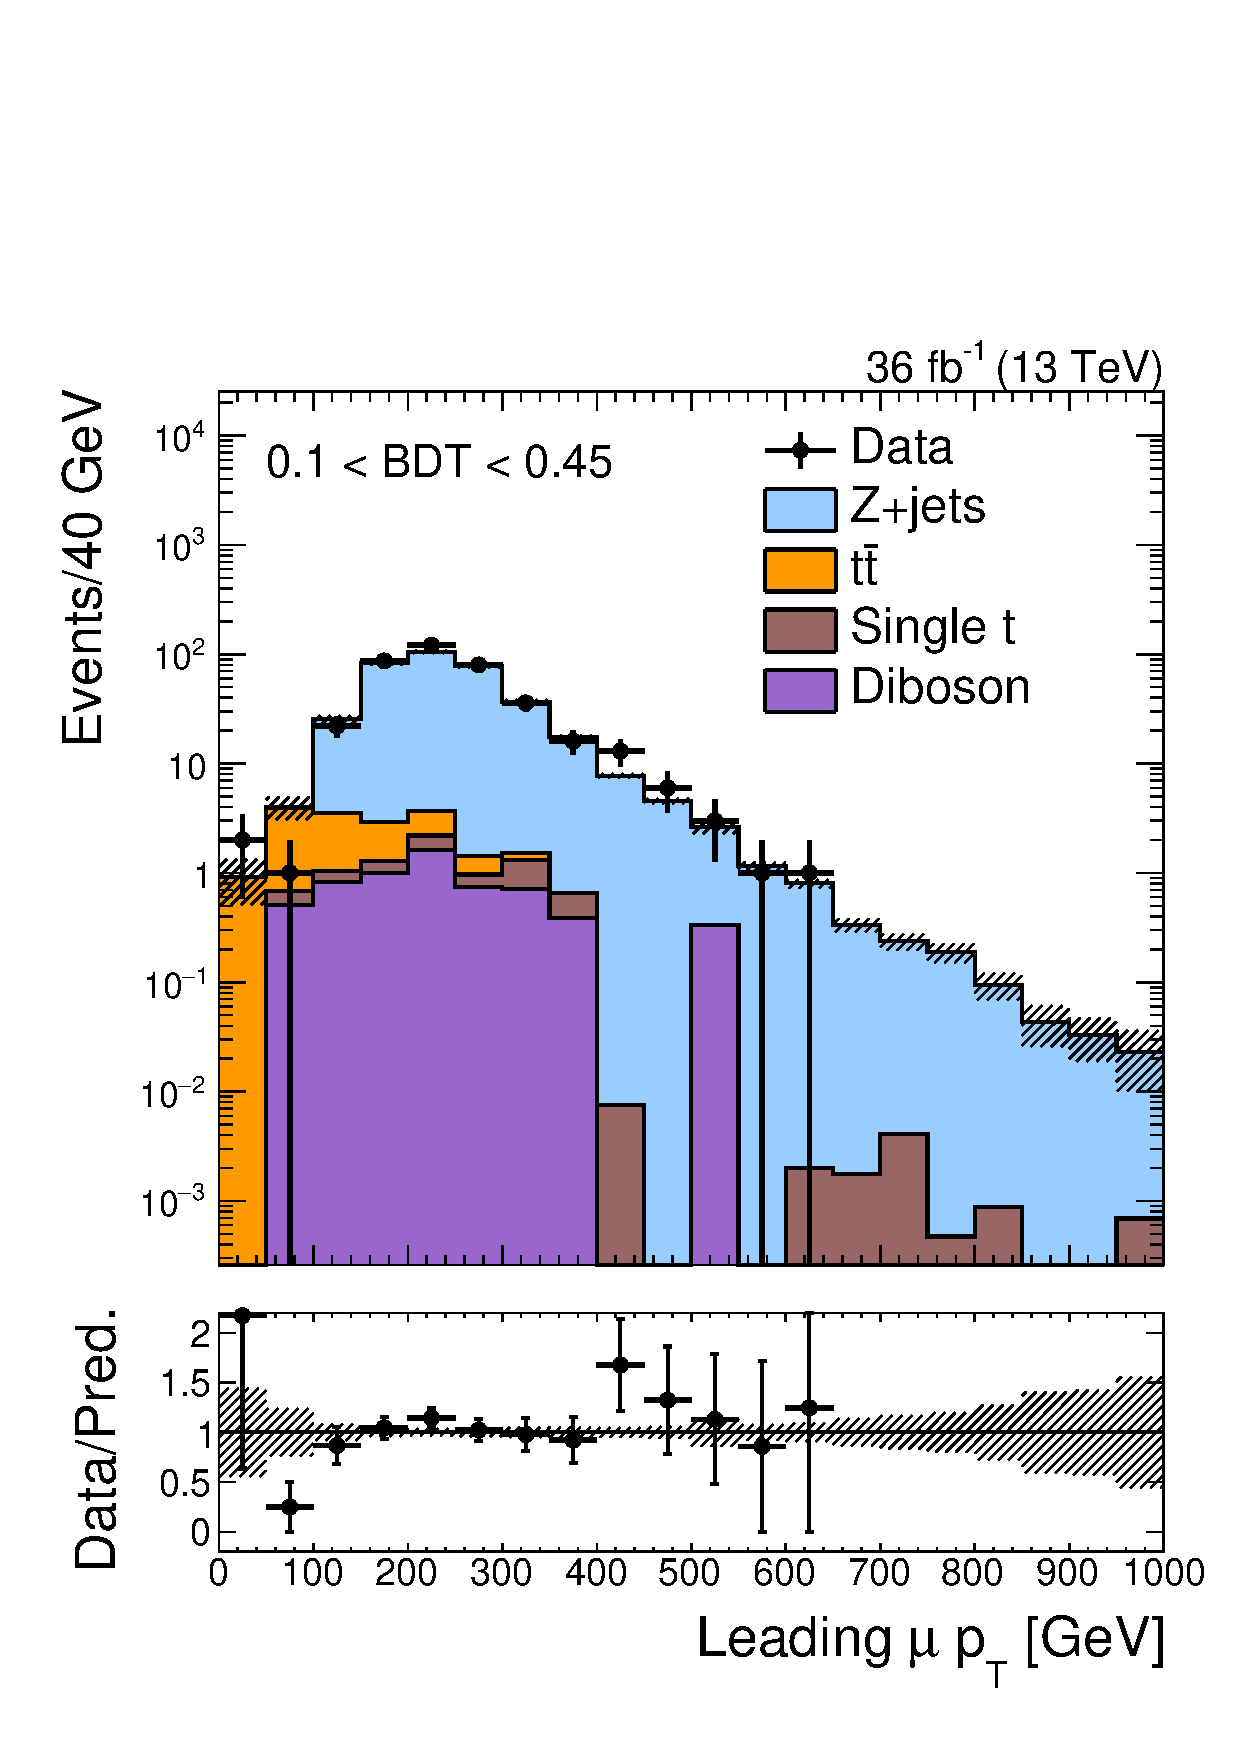
\includegraphics[width=\textwidth]{figures/monotop/prefit/dimuon_loose_looseLep1Pt_logy.pdf}
            \caption{Leading muon $\pt$}
        \end{subfigure}
        \caption{Various kinematic distributions in the two mono-top $\mu\mu$ CRs. 
                Note the clearly discernable peak in the $m_{\mu\mu}$ distribution near $m_Z$}
        \label{fig:mt:prefit_dimuon}
    \end{center}
\end{figure}

The control data is used to constrain the SR prediction by means of ``transfer factors'' $\Ti{X}{Y}$, where $X$ refers to a particular CR (e.g. $\mu\mu$), $Y$ refers to a particular process (e.g. $Z$), and $i$ refers to a particular bin in the CR (e.g. $200<U<250$ GeV in the tight category).
Formally:
\begin{equation}
    \Ti{\mu\mu}{Z} = \frac{N^\mathrm{SR}_i(Z\rightarrow\nu\nu)}{N^{\mu\mu}_i(Z\rightarrow\mu\mu)}
\end{equation}
The transfer factors are estimated using MC simulation.
To encode the effects of various uncertainties, we introduce nuisance parameters $\bm{\theta}$.
That is:
\begin{gather}
    \Ti{X}{Y} \rightarrow \Ti{X}{Y}(\bm\theta) \equiv \Ti{X}{Y} \times \prod_{j=0}^{n_\theta} (1+\theta_j) \\ 
    \theta_j \sim p_j(\theta_j) 
\end{gather}
where $n_\theta$ is the number of nuisance parameters and $p_j(\theta_j)$ is some prior distribution for each nuisance (see below for how the priors are used).
The priors are typically chosen to have a central value (e.g. mean, median) at $0$, with a finite variance that encodes the uncertainty.
In this chapter, we assume $p_j$ is either a normal distribution centered at 0 or a log-normal distribution (in cases where negative values are undesirable). 
We will use the terms ``uncertainty'' and ``nuisance parameter'' interchangeably. 

Let $\pois(d|\lambda)$ refer to the Poisson probability of observing $d$ with an expected mean of $\lambda$. 
In terms of these transfer factors, the likelihood for the data observed in the signal and $\mu\mu$ control regions is:
\begin{align}
    \mathcal{L}(\bm{d} ~|~ \mu,\muz,\bm{\theta}) = & \prod_{i\in\mathrm{bins}} \left[ 
    \pois\left(d^{\mathrm{SR}}_{i} ~|~ \mu S^{\mathrm{SR}}_{i}(\bm\theta)  + \muzi + B^{\mathrm{SR}}_{i}(\bm\theta)\right) \vphantom{\frac{\muzi}{\Ti{\mu\mu}{Z}(\bm\theta)}}\right. \nonumber \\
    & \left. \phantom{\prod_{i\in\mathrm{bins}}\Big[} \times \pois\left(d^{\mu\mu}_i~\Big|~ \frac{\muzi}{\Ti{\mu\mu}{Z}(\bm\theta)} + B^{\mu\mu}_i(\bm\theta) \right)\right]  \times  \prod_{j=0}^{n_\theta} p_j(\theta_j)
\end{align}
where the following notation is used:
\begin{itemize}
    \item[$d^X_i$]: The data observed in bin $i$ of region $X$. For now, $X=\mathrm{SR},\mu\mu$. 
    \item[$S^\mathrm{SR}_i$]: The predicted number of signal events in bin $i$ of the SR, under some fixed signal hypothesis. 
    \item[$\mu$]: The ``signal strength''. Essentially an unconstrained nuisance parameter that scales up or down the total signal yield. 
    \item[$\mu_{\mathrm{SR},i}^P$]: The expected number of events from process $P$ in bin $i$ of the SR. This is also an unconstrained nuisance parameter. 
    \item[$B^X_i$]: The predicted number of ``minor'' background events in bin $i$ of region $X$. Here, ``minor'' refers to all SM processes that are not the signal and are not estimated using a data-driven method. 
\end{itemize}
The signal and background yields $\bm{S}$ and $\bm{B}$ are estimated using MC.
Note that the inclusion of the priors in the likelihood constrains the nuisance parameters to be close to their ``nominal'' values; moving a $\theta_j$ to fit the data incurs a large cost from the prior.

If we set $B_i = \mu = 0$ (the null hypothesis, ignoring small minor backgrounds), a simple picture emerges of how the likelihood is maximized.
The parameters $\muz$ float freely to satisfy $d_\mathrm{SR,i} \sim \muzi$ and $d_\mathrm{\mu\mu,i}\sim \muzi / \Ti{\mu\mu}{Z}(\bm\theta)$. 
If both constraints cannot be satisfied simultaneously by scaling $\muz$, the (constrained) nuisance parameters $\bm\theta$ modify the transfer factor $\T{\mu\mu}{Z}$. 
Table~\ref{tab:mt:zmm_uncs} shows the relevant uncertainties for $\T{\mu\mu}{Z}$, and Figure~\ref{fig:mt:zmm_uncs} shows the shape of uncertainties that evolve as a function of $U$.

\begin{table}[]
    \begin{center}
    \caption{Uncertainties affecting the $\mu\mu$ $\leftrightarrow$ $\nu\nu$ extrapolation. ``Shape'' uncertainties have different priors for each bin, but are assumed to be correlated across bins.}
    \label{tab:mt:zmm_uncs}
    \begin{tabular}{lcl}
        Uncertainty & 1 s.d. & Notes \\ 
        \hline \hline 
        $\mu$ ID  & 2\% & \\ 
        $\mu$ track  & 1\% & \\ 
        $\tau_\mathrm{h}$ veto  & 3\% & \\ 
        $Z$+heavy flavor & 3\% & \\ 
        Trigger & 0-2\% & Shape \\ 
        $b$-tag & $\sim0.5\%$ & Shape \\ 
        $udcsg$-mistag & 3-4\% & Shape \\ 
    \end{tabular}
\end{center}
\end{table}


\begin{figure}[]
    \begin{center}
        \begin{subfigure}[t]{0.49\textwidth}
            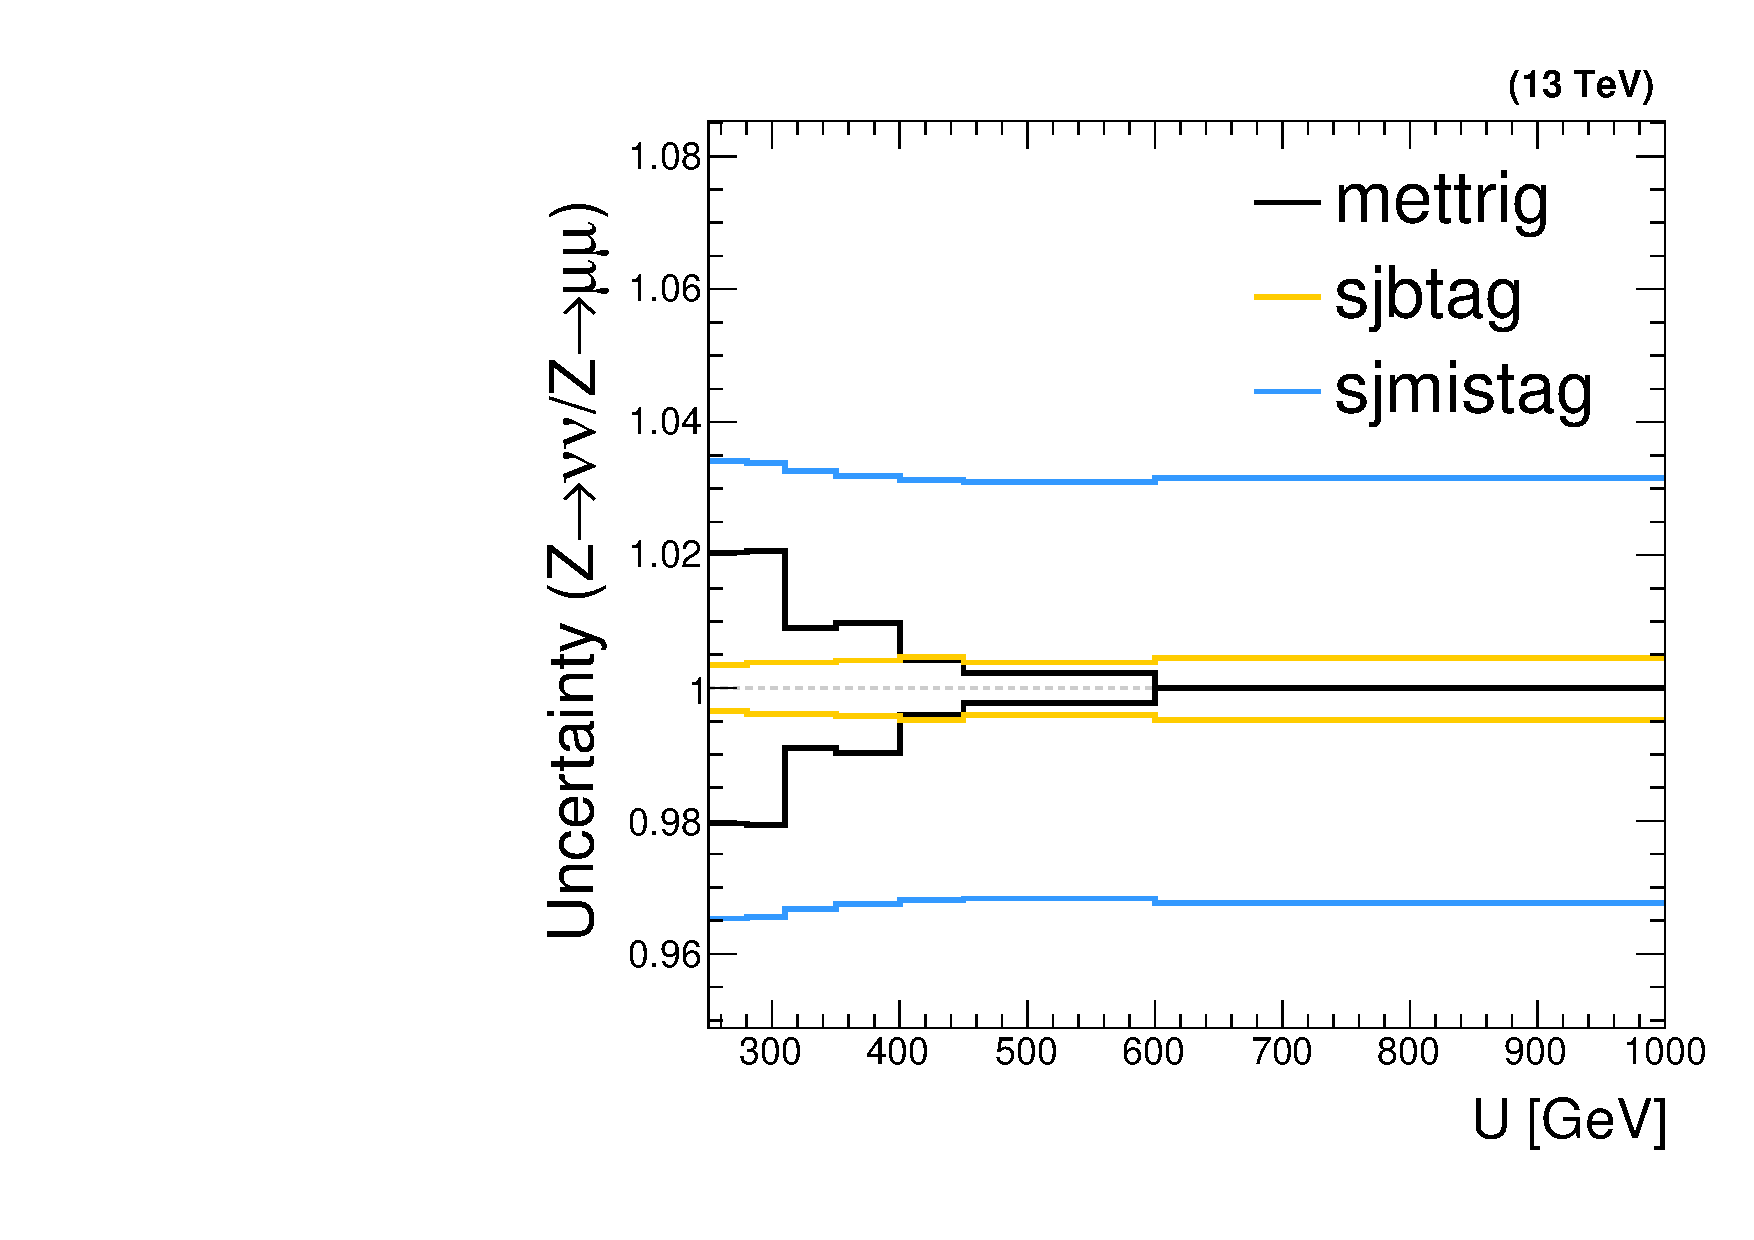
\includegraphics[width=\textwidth]{figures/monotop/uncertainties/variations_dimuon_loose.pdf}
            \caption{Loose}
        \end{subfigure}
        \begin{subfigure}[t]{0.49\textwidth}
            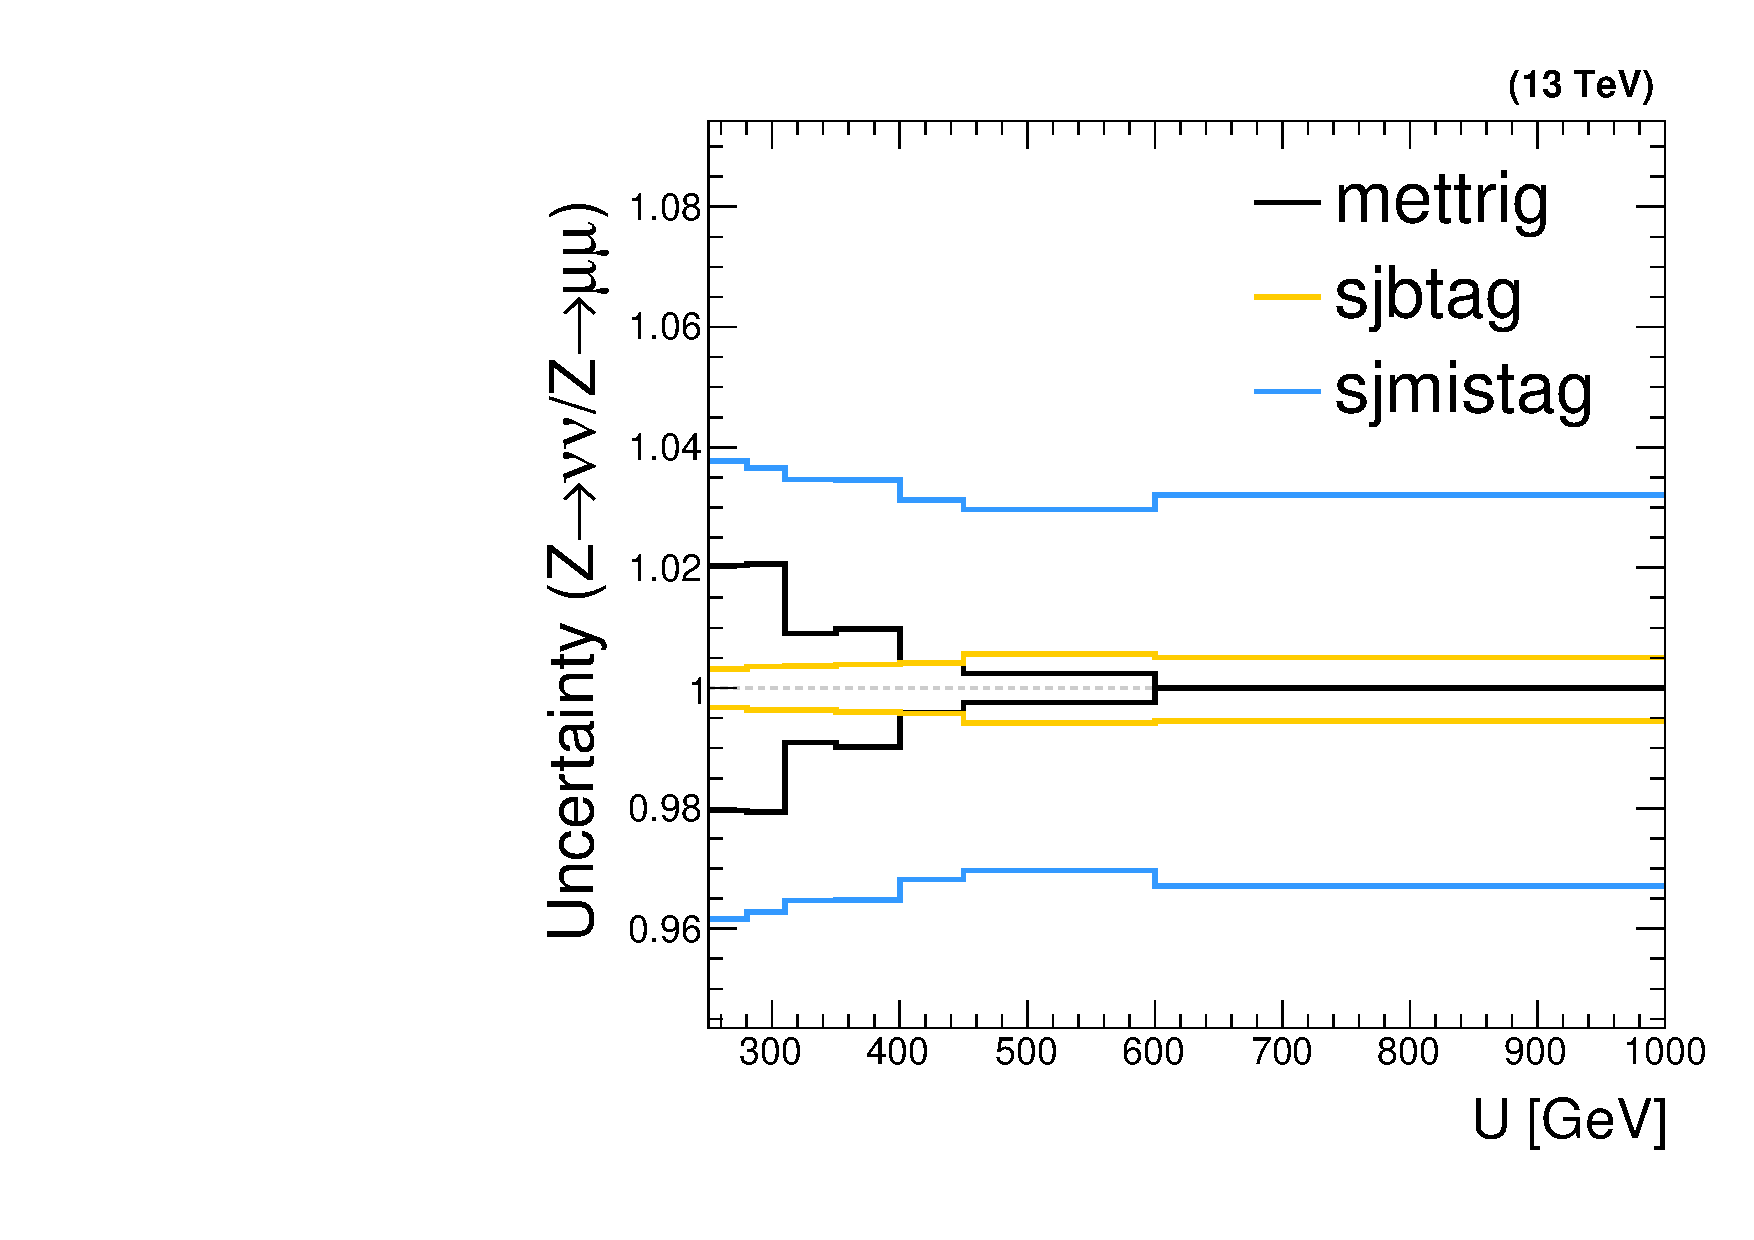
\includegraphics[width=\textwidth]{figures/monotop/uncertainties/variations_dimuon.pdf}
            \caption{Tight}
        \end{subfigure}
        \caption{Shape uncertainties affecting $T_i^{\mu\mu}$ in both categories, as a function of $U$.}
        \label{fig:mt:zmm_uncs}
    \end{center}
\end{figure}

The transfer factors are shown in Figure~\ref{fig:mt:zmm_xfer}.  
The exact values of $\T{\mu\mu}{Z}(\bm\theta)$ have two salient features:
\begin{enumerate}
    \item The values are strictly greater than one. 
        This is due to (a) $\mathcal{B}(Z\rightarrow\nu\nu)>\mathcal{B}(Z\rightarrow\mu\mu)$ and (b) a non-100\% efficiency in reconstructing and identifying muons. 
        This implies that the constraining power of the $\mu\mu$ CR is less than that of the SR, especially at high $U$ (i.e. the Poisson uncertainties are larger). 
    \item The one standard deviation variation of all uncertainties that impact $\Ti{\mu\mu}{Z}$ are contained within a 10\% envelope. 
        This is already a factor of two smaller than the inherent $\sim20\%$ uncertainties in the MC simulation.
\end{enumerate}

\begin{figure}[]
    \begin{center}
        \begin{subfigure}[t]{0.49\textwidth}
            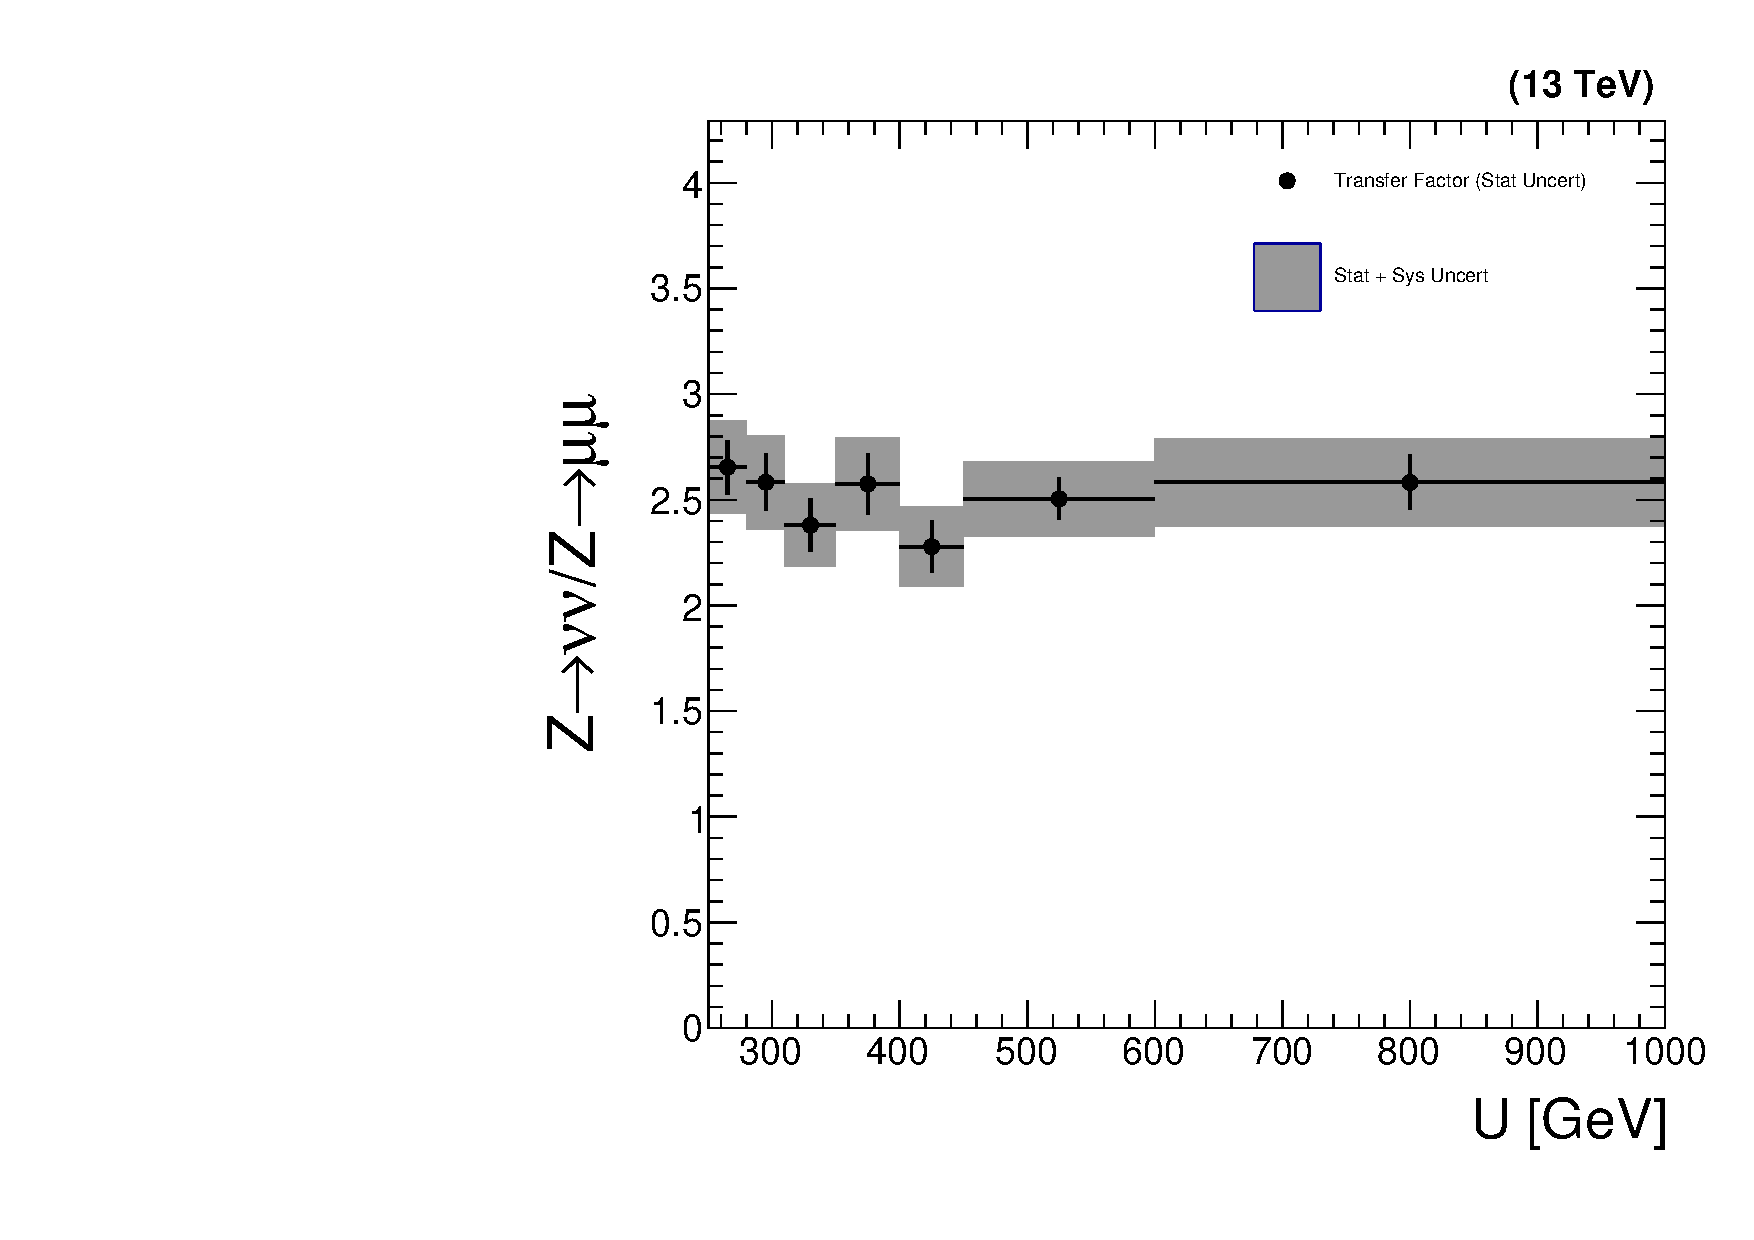
\includegraphics[width=\textwidth]{figures/monotop/xfer/rfactor_dimuon_loose.pdf}
            \caption{Loose}
        \end{subfigure}
        \begin{subfigure}[t]{0.49\textwidth}
            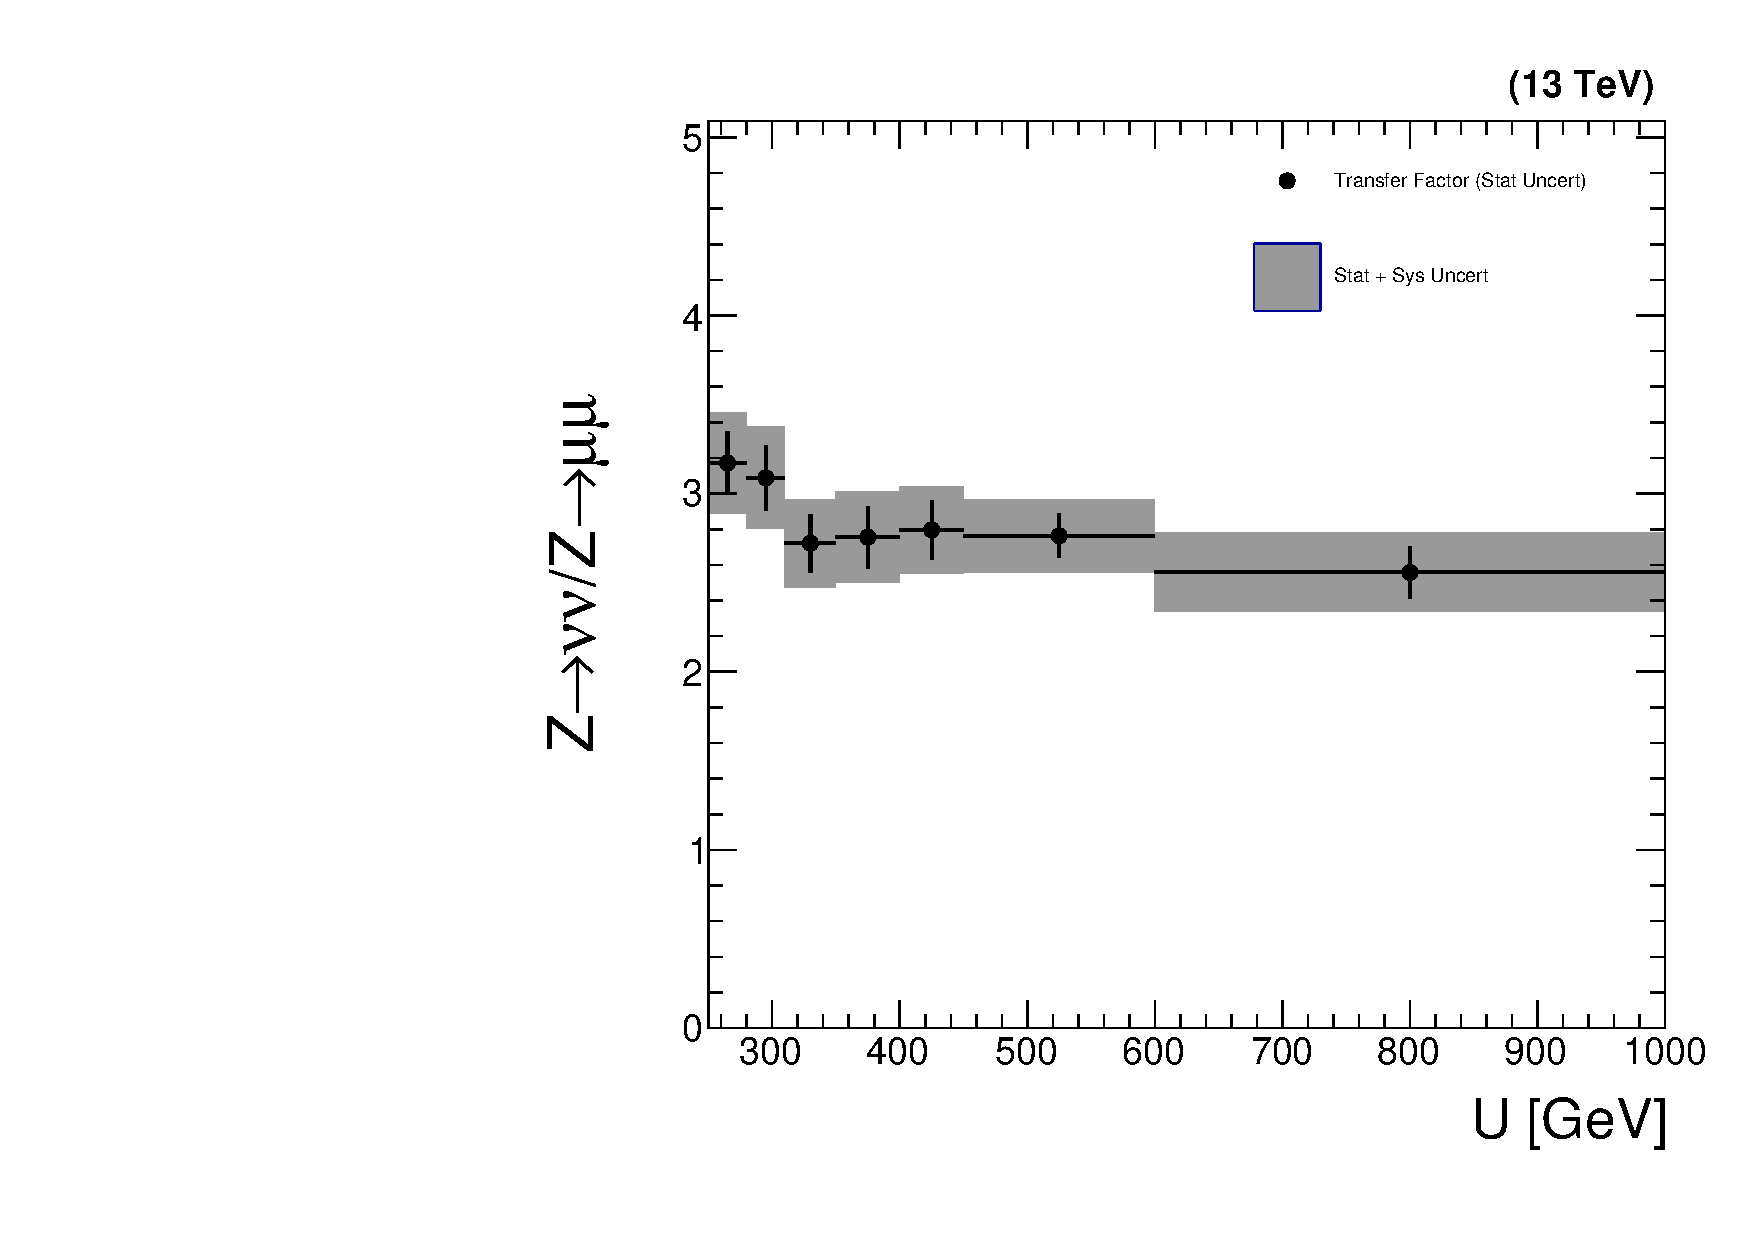
\includegraphics[width=\textwidth]{figures/monotop/xfer/rfactor_dimuon.pdf}
            \caption{Tight}
        \end{subfigure}
        \caption{The transfer factors $\Ti{\mu\mu}{Z}$ as a function of recoil and BDT score. The vertical black bars represent the Poisson uncertainties in the MC simulation, while the grey bands represent the sum of Poisson uncertainties and other, systematic, uncertainties. All uncertainties are represented as one standard deviation.}
        \label{fig:mt:zmm_xfer}
    \end{center}
\end{figure}

To account for point (1), we can simply add more control data by also looking at $Z\rightarrow ee$ decays. 
Essentially all of the arguments used for the $\mu\mu$ CRs applies to the $ee$ CRs. 
Figures~\ref{fig:mt:prefit_dielectron}-\ref{fig:mt:zee_xfer} show the data/simulation agreement and the transfer factors for the new dielectron regions.
A further set of statistical constraints to improve the estimate at high $U$ (which is where the signals are most enhanced) is described in Section~\ref{sec:mt:smtheory}. 

\begin{figure}[]
    \begin{center}
        \begin{subfigure}[t]{0.32\textwidth}
            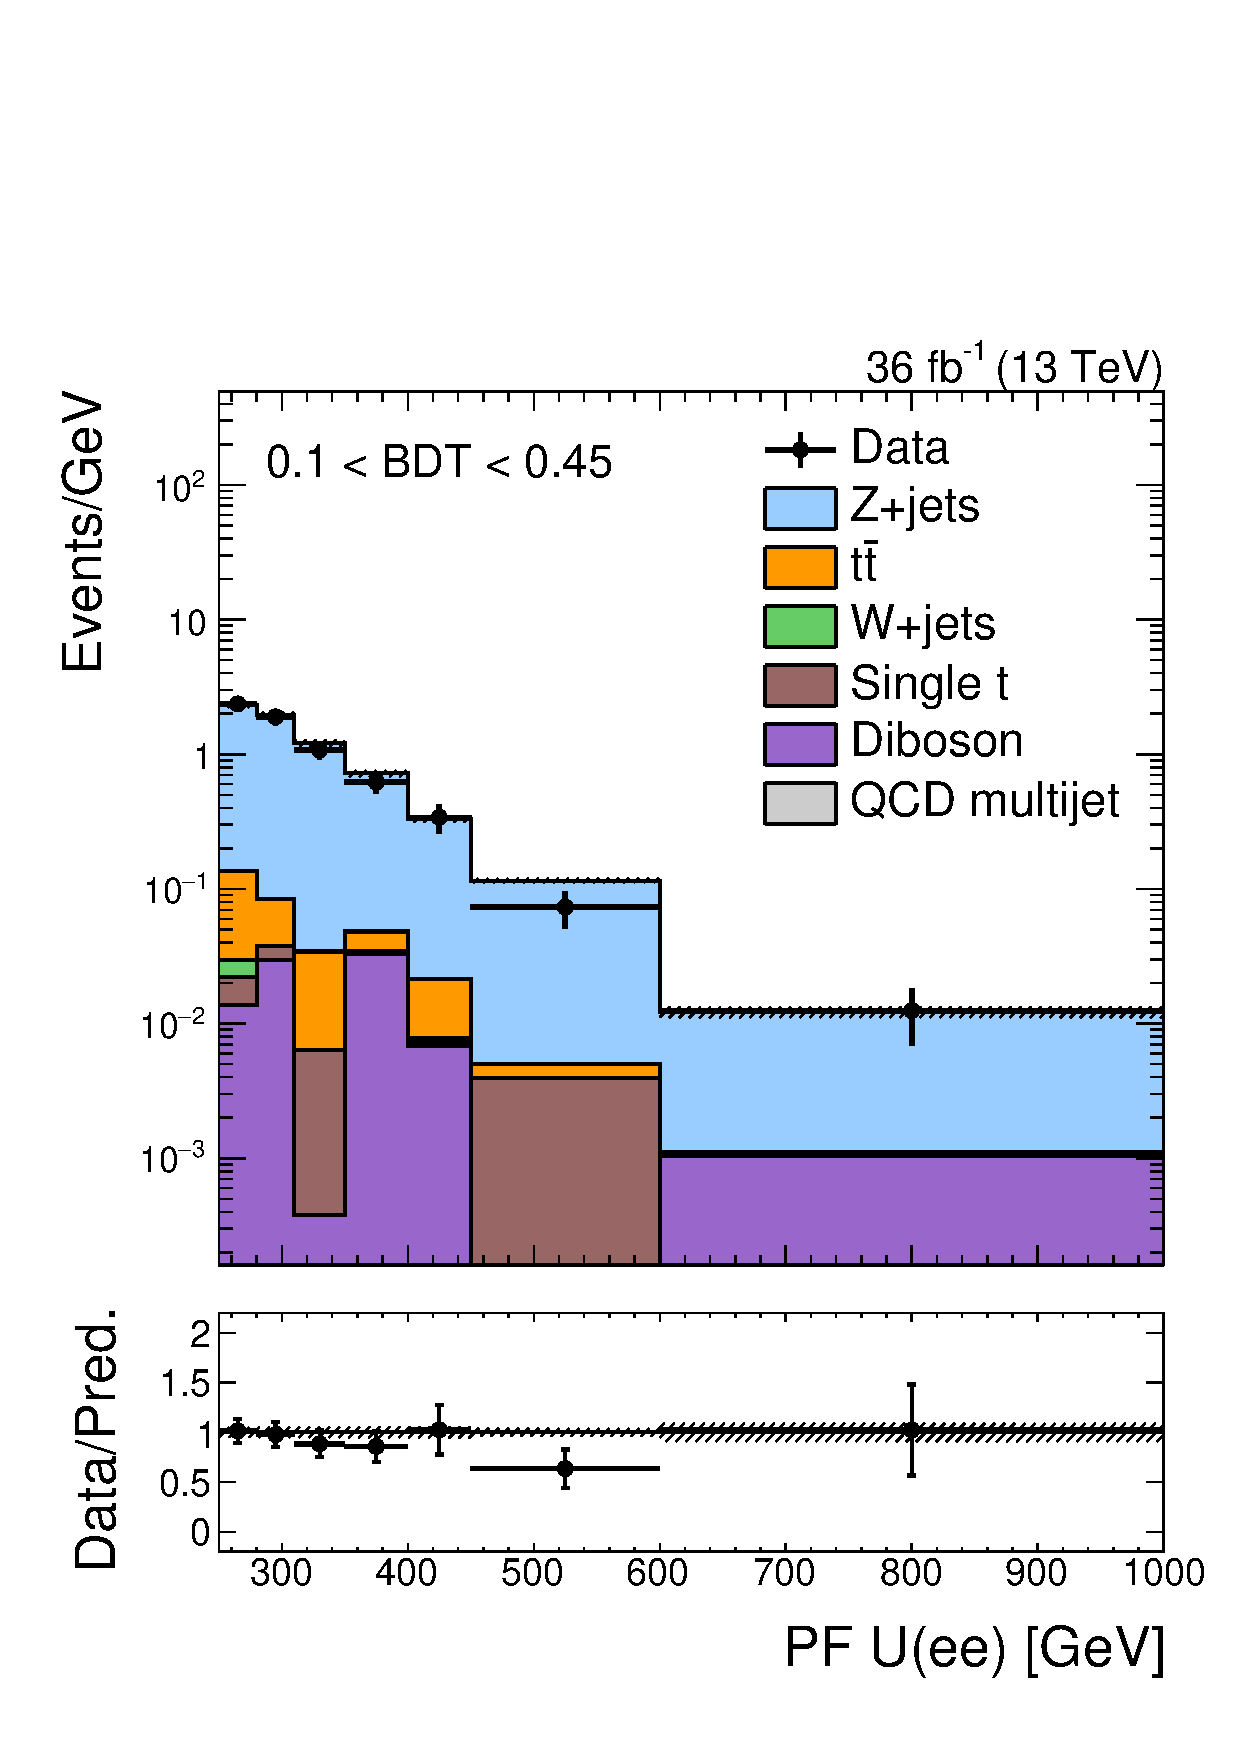
\includegraphics[width=\textwidth]{figures/monotop/prefit/dielectron_loose_pfUZmag_logy.pdf}
            \caption{$U$ in loose CR}
        \end{subfigure}
        \begin{subfigure}[t]{0.32\textwidth}
            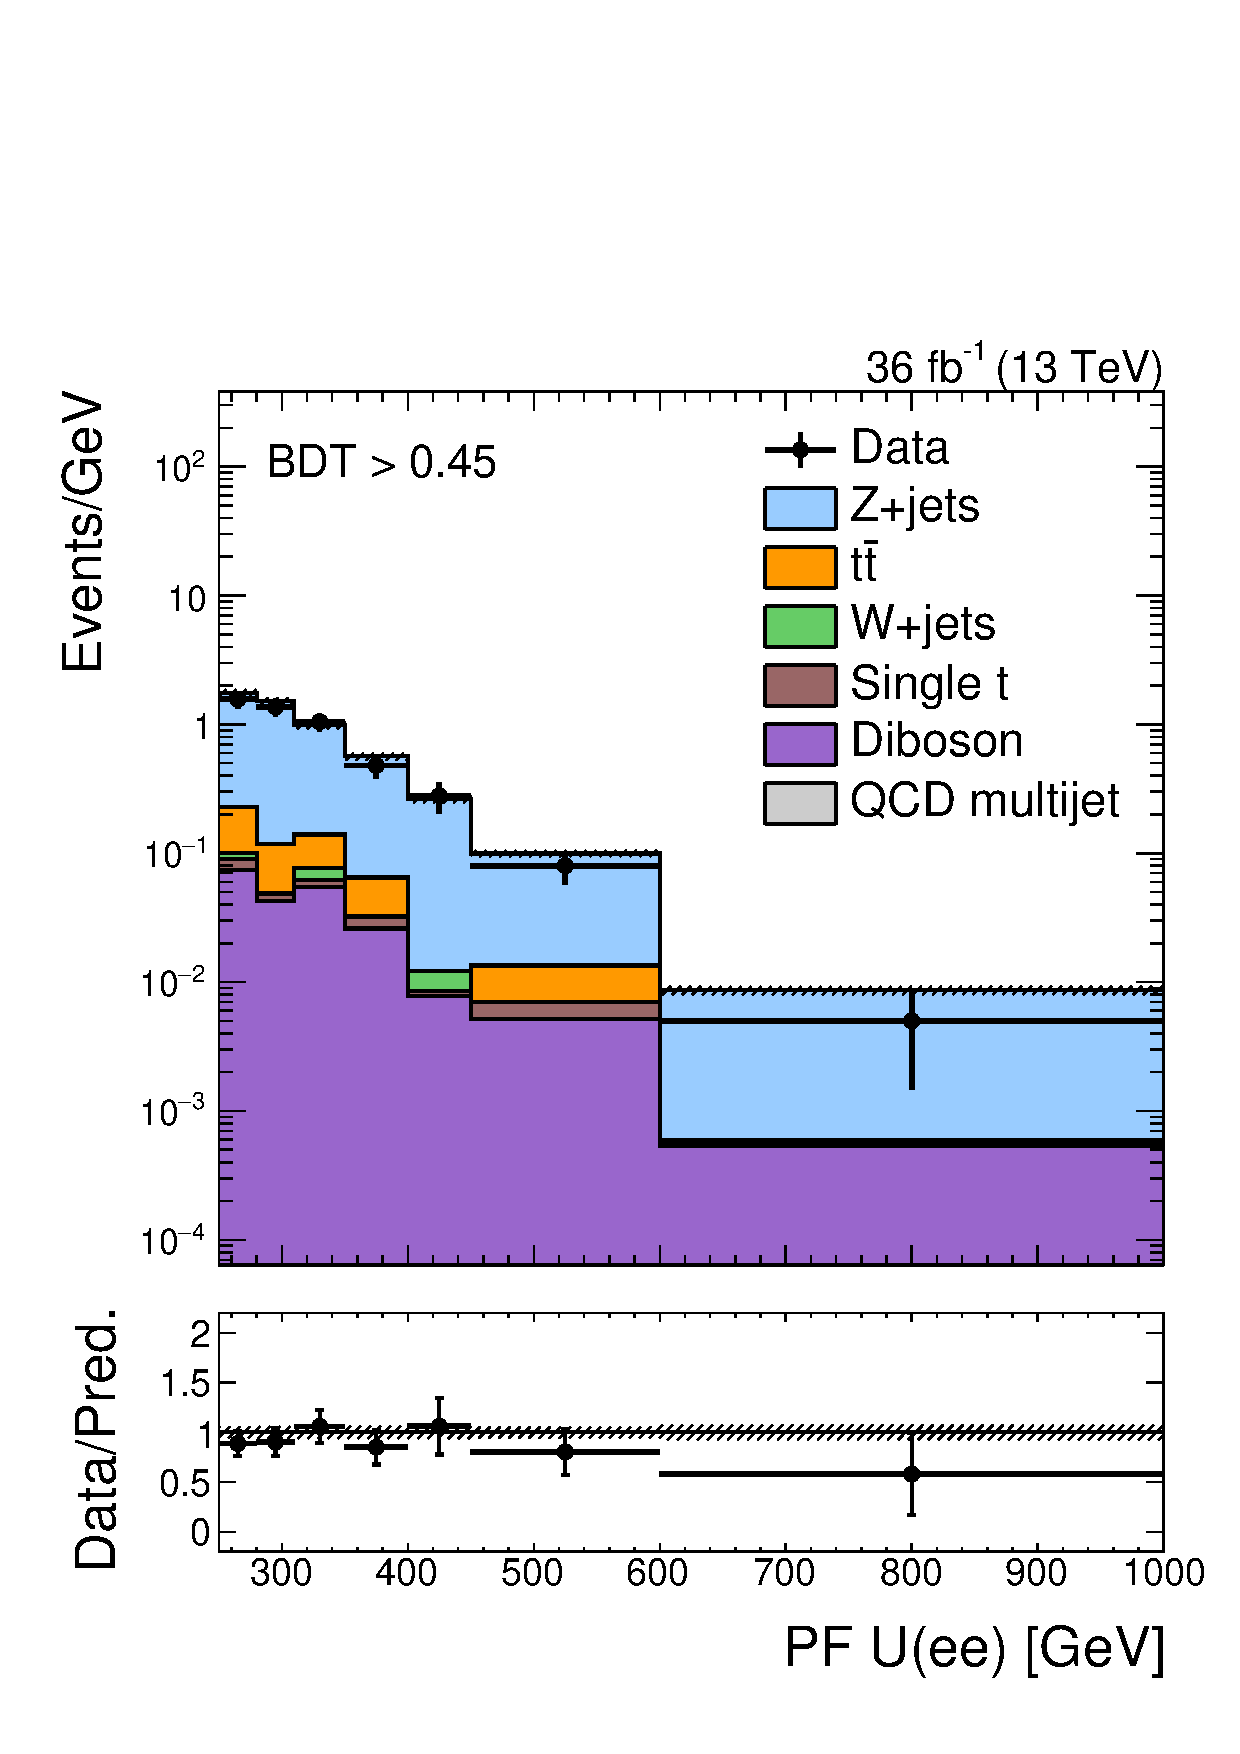
\includegraphics[width=\textwidth]{figures/monotop/prefit/dielectron_tight_pfUZmag_logy.pdf}
            \caption{$U$ in tight CR}
        \end{subfigure}
        \begin{subfigure}[t]{0.32\textwidth}
            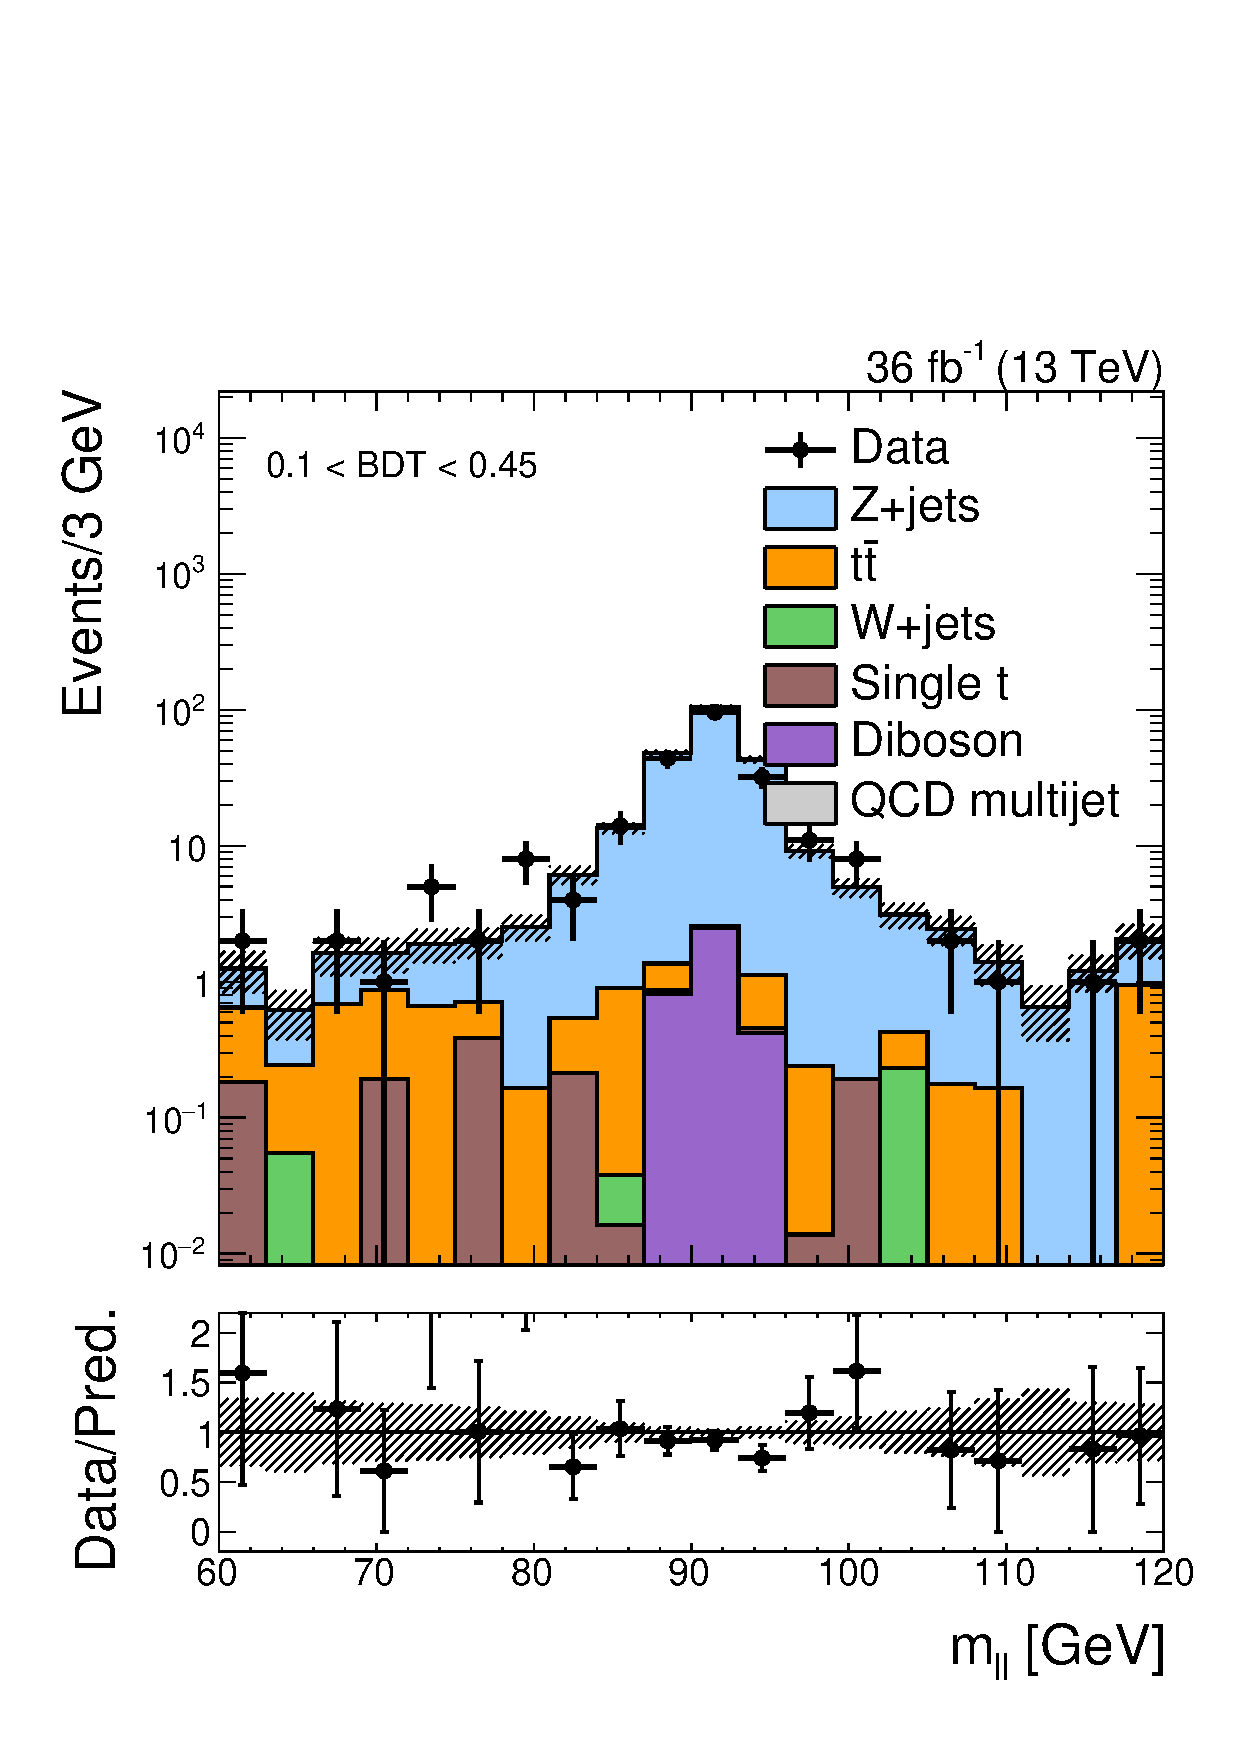
\includegraphics[width=\textwidth]{figures/monotop/prefit/dielectron_loose_diLepMass_logy.pdf}
            \caption{$m_{ee}$}
        \end{subfigure}
        \caption{Various kinematic distributions in the two mono-top $ee$ CRs. }
        \label{fig:mt:prefit_dielectron}
    \end{center}
\end{figure}

\begin{figure}[]
    \begin{center}
        \begin{subfigure}[t]{0.49\textwidth}
            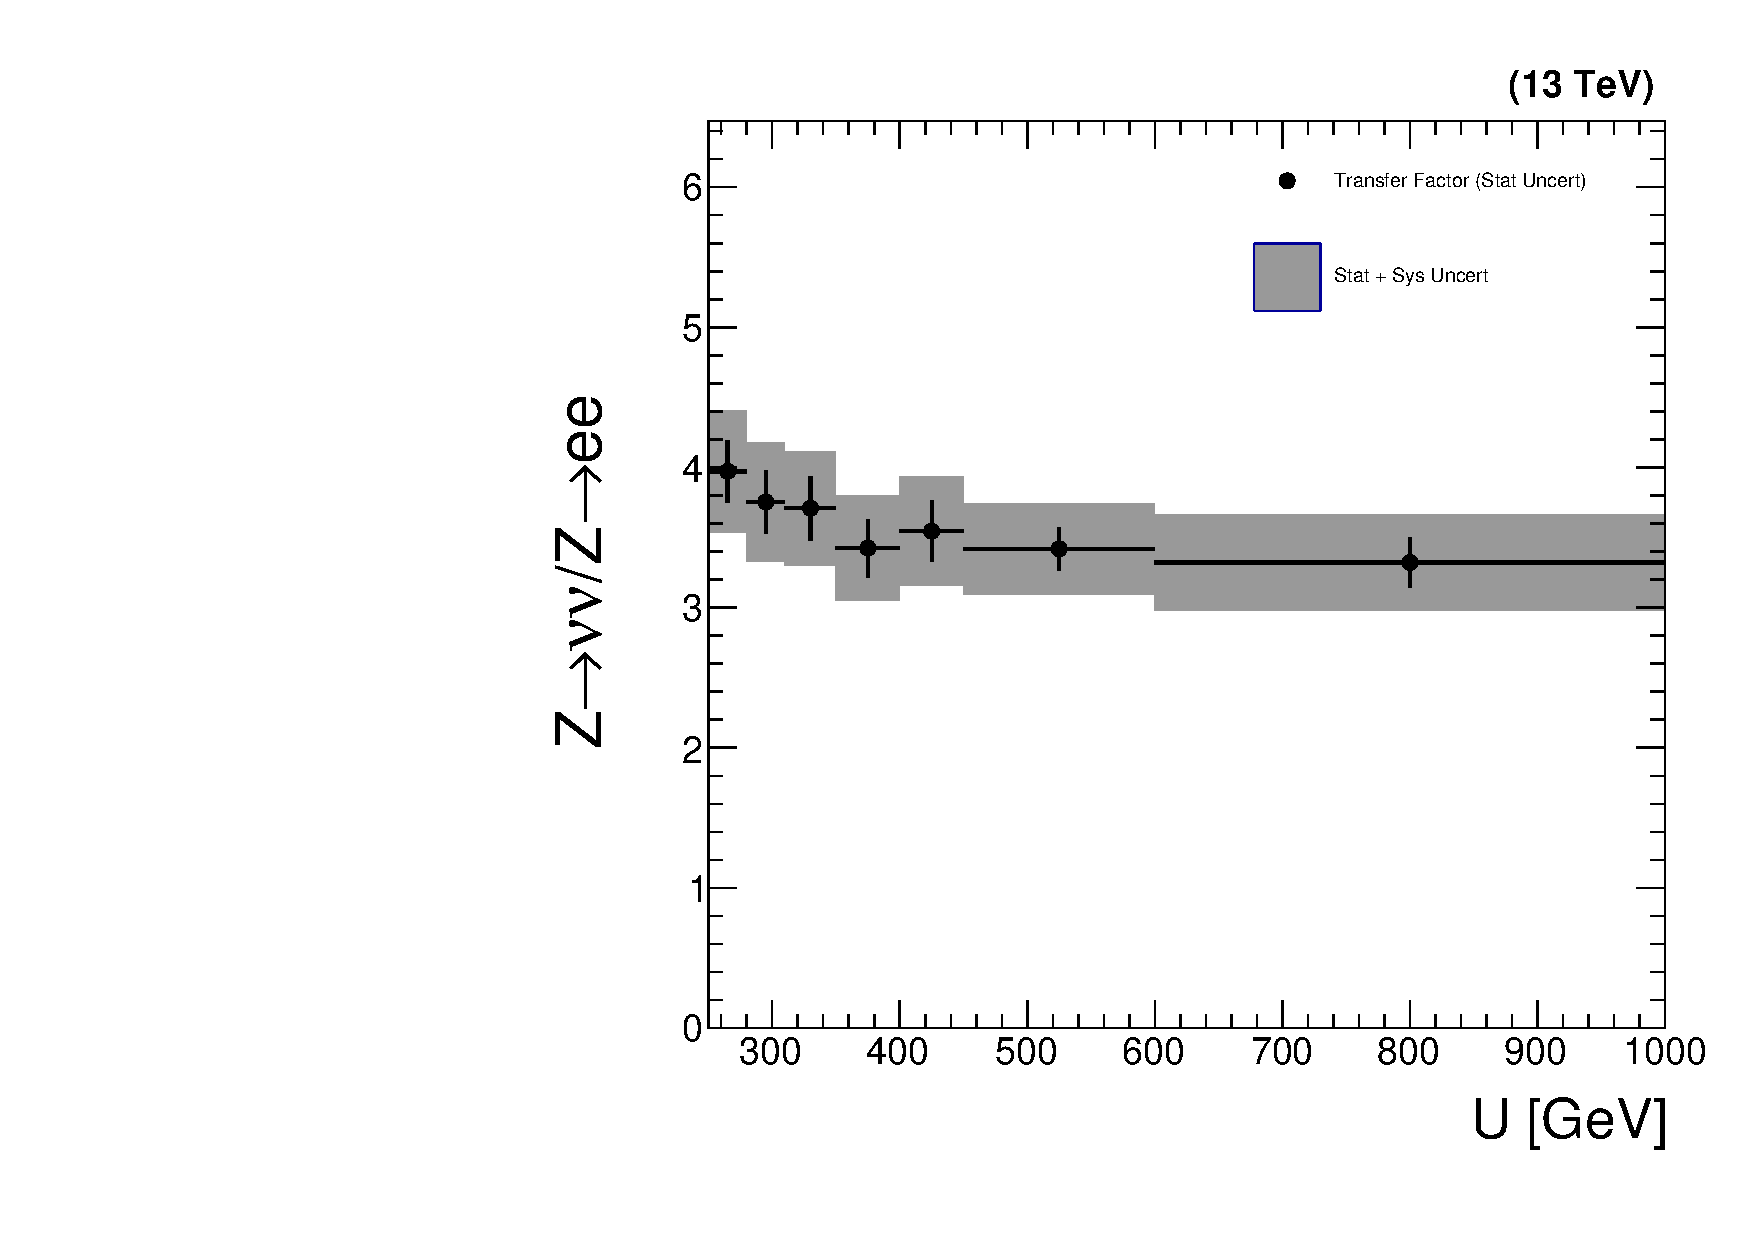
\includegraphics[width=\textwidth]{figures/monotop/xfer/rfactor_dielectron_loose.pdf}
            \caption{Loose}
        \end{subfigure}
        \begin{subfigure}[t]{0.49\textwidth}
            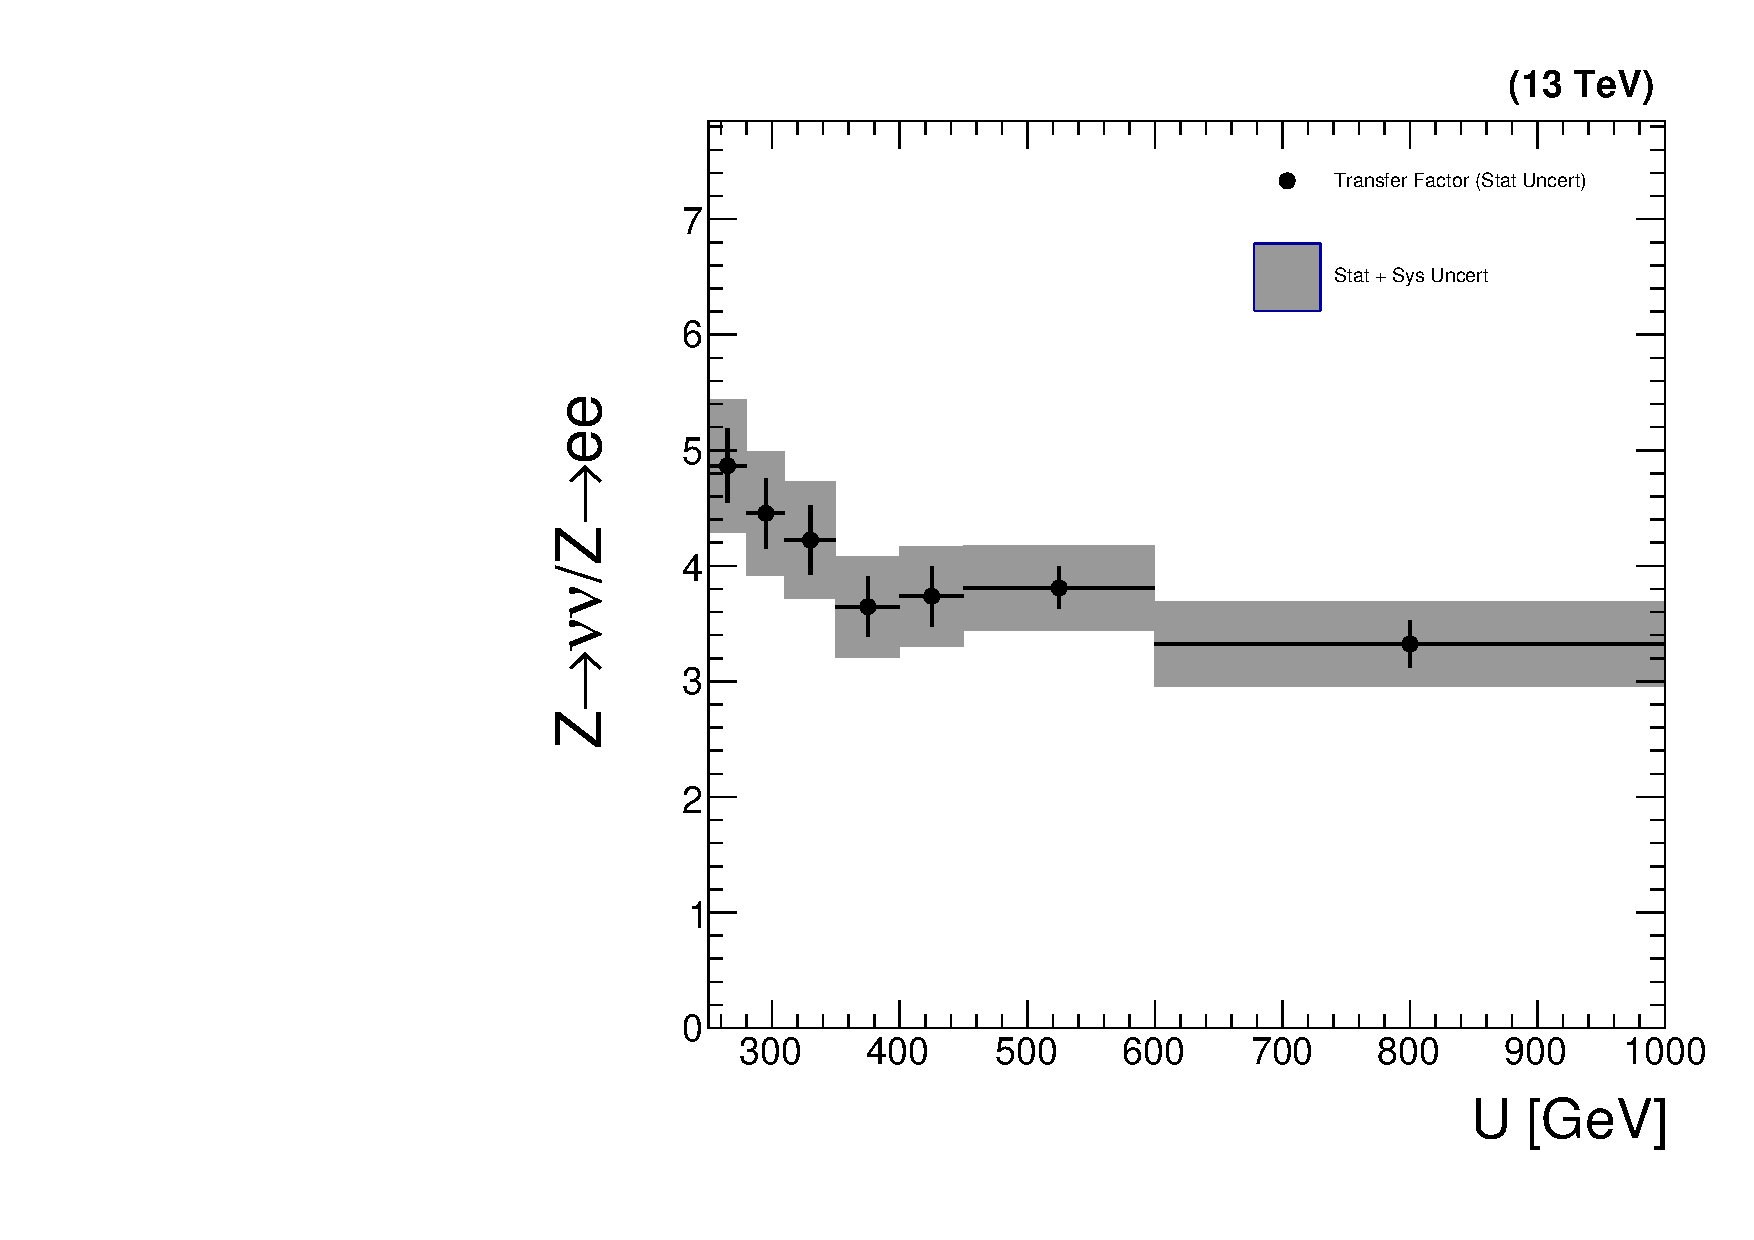
\includegraphics[width=\textwidth]{figures/monotop/xfer/rfactor_dielectron.pdf}
            \caption{Tight}
        \end{subfigure}
        \caption{The transfer factors $T_i^{ee}$ as a function of recoil and BDT score. The vertical black bars represent the Poisson uncertainties in the MC simulation, while the grey bands represent the sum of Poisson uncertainties and other, systematic, uncertainties. All uncertainties are represented as one standard deviation.}
        \label{fig:mt:zee_xfer}
    \end{center}
\end{figure}

Similar methods are used to predict the $W$+jets and $t\bar{t}$ contributions in the SRs; these three backgrounds comprise at least $95\%$ of the SM processes.
In both cases, the momentum imbalance in the SR is a proxy for the momentum of the $W$ boson, since the charged lepton is lost.
A sketch of the event topologies is shown in Figure~\ref{fig:mt:wtt}.
Following the same arguments as used for the $Z\rightarrow\ell\ell$ CRs, we can use the hadronic recoil $U$ in CRs that measure visible final states of $W$ and $t\bar{t}$.

\begin{figure}[]
    \begin{center}
        \begin{subfigure}[t]{0.49\textwidth}
            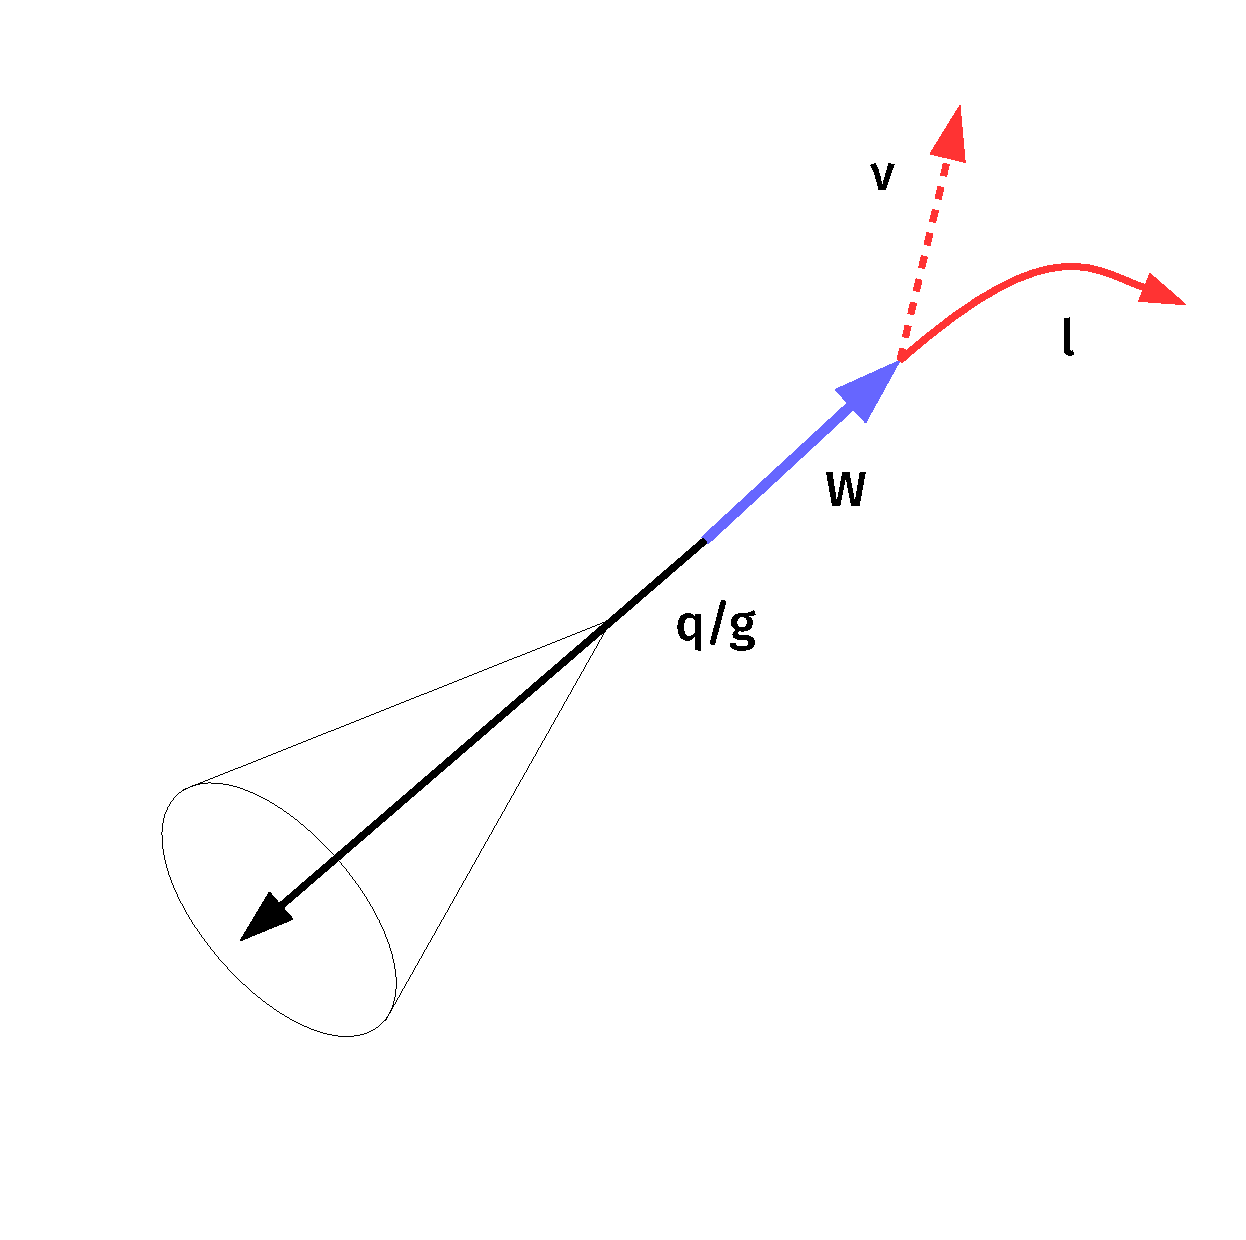
\includegraphics[width=\textwidth]{figures/monotop/diagrams/wcr.pdf}
            \caption{$W\rightarrow\ell\nu$}
        \end{subfigure}
        \begin{subfigure}[t]{0.49\textwidth}
            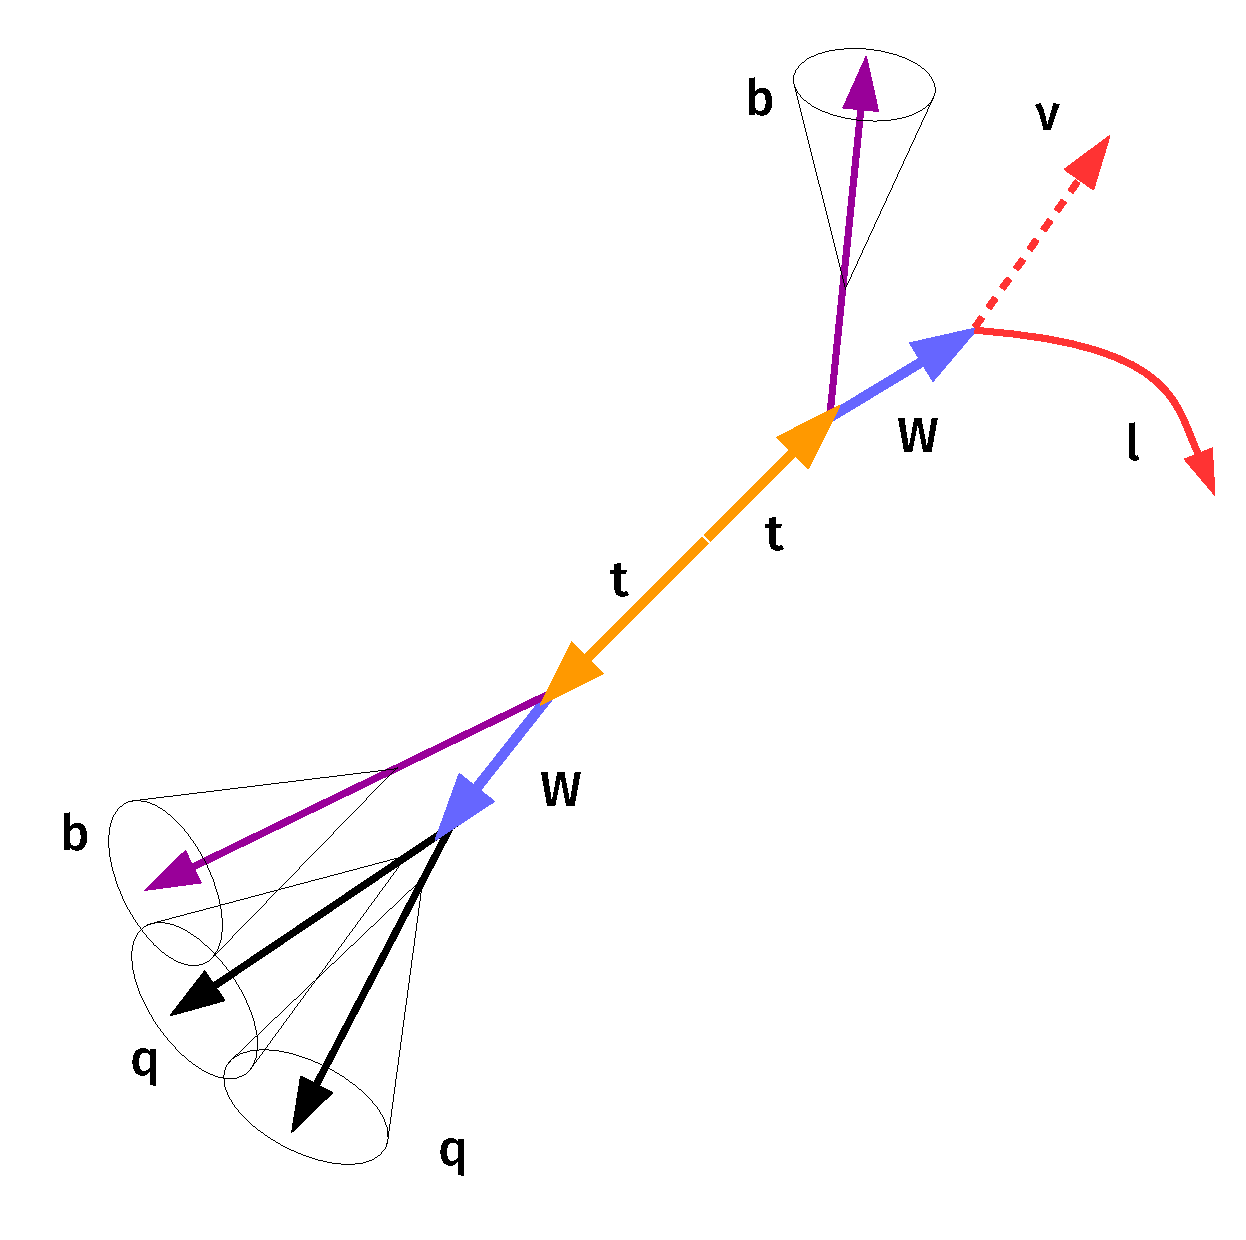
\includegraphics[width=\textwidth]{figures/monotop/diagrams/ttcr.pdf}
            \caption{$t\bar{t}\rightarrow bqq'+b\ell\nu$}
        \end{subfigure}
        \caption{Schematic representation of the $W$ and $t\bar{t}$ SM processes. 
                 In both cases, $U\approx \pt^W$.
                 Furthermore, if the charged lepton is lost, $U = \ptmiss \approx \pt^W$.}
        \label{fig:mt:wtt}
    \end{center}
\end{figure}

Starting with muon final states (electrons will follow naturally), we define two sets of CRs based on the number of identified $B$ hadrons.
The selection for the $b\mu$ CRs (to measure $t\bar{t}$) is shown in Table~\ref{tab:mt:tmn_cuts}.
The selection for the $\mu$ CRs (to measure $W$) is shown in Table~\ref{tab:mt:wmn_cuts}.
Figures~\ref{fig:mt:prefit_tmn}-\ref{fig:mt:prefit_wmn} show various kinematic distributions in these regions. 

\begin{table}[]
    \caption{Criteria used to select events for the mono-top $b\mu$ CR. As with the SR, the region is further split based on the jet BDT score.}
    \label{tab:mt:tmn_cuts}
    \centering
    \begin{tabular}{p{0.4\textwidth}p{0.6\textwidth}}
        Criterion & Notes \\ 
        \hline 
        \hline 
        $U>250$ GeV & Mimicking the selection in the SR; also constrained by trigger thresholds. \\ 
        1 CA15 jet with $\pt>250$ GeV &  Same as SR \\ 
        CA15 jet $110 < m_\mathrm{SD} < 210$ GeV & Same as SR \\ 
        At least one $b$-tagged sub-jet & Identifying $B$ hadron produced from hadronic top decay. \\ 
        Exactly one $b$-tagged narrow jet & Identifying $B$ hadron produced from leptonic top decay. \\ 
        \hline 
        Exactly one well-identified $\mu$ & Produced from $W\rightarrow\mu\nu$ \\ 
        No identified $e,\tau_\mathrm{h}$ & Same as SR. \\ 
        No identified $\gamma$ & Same as SR \\ 
        \hline 
        $\min_\mathrm{jets}\Delta\phi(\mathrm{jet},U) > 0.5$ & Same as SR \\ 
        \hline 
        CA15 jet BDT & Same as SR\\ 
    \end{tabular}
\end{table}

\begin{table}[]
    \caption{Criteria used to select events for the mono-top $\mu$ CR. As with the SR, the region is further split based on the jet BDT score.}
    \label{tab:mt:wmn_cuts}
    \centering
    \begin{tabular}{p{0.4\textwidth}p{0.6\textwidth}}
        Criterion & Notes \\ 
        \hline 
        \hline 
        $U>250$ GeV & Mimicking the selection in the SR; also constrained by trigger thresholds. \\ 
        1 CA15 jet with $\pt>250$ GeV &  Same as SR \\ 
        CA15 jet $110 < m_\mathrm{SD} < 210$ GeV & Same as SR \\ 
        No $b$-tagged sub-jets & Suppressing semi-leptonic $t\bar{t}$ decays \\ 
        No $b$-tagged narrow jets & Suppressing semi-leptonic $t\bar{t}$ decays \\ 
        \hline 
        Exactly one well-identified $\mu$ & Produced from $W\rightarrow\mu\nu$ \\ 
        No identified $e,\tau_\mathrm{h}$ & Same as SR. \\ 
        No identified $\gamma$ & Same as SR \\ 
        \hline 
        $\min_\mathrm{jets}\Delta\phi(\mathrm{jet},U) > 0.5$ & Same as SR \\ 
        \hline 
        CA15 jet BDT & Same as SR\\ 
    \end{tabular}
\end{table}

\begin{figure}[]
    \begin{center}
        \begin{subfigure}[t]{0.32\textwidth}
            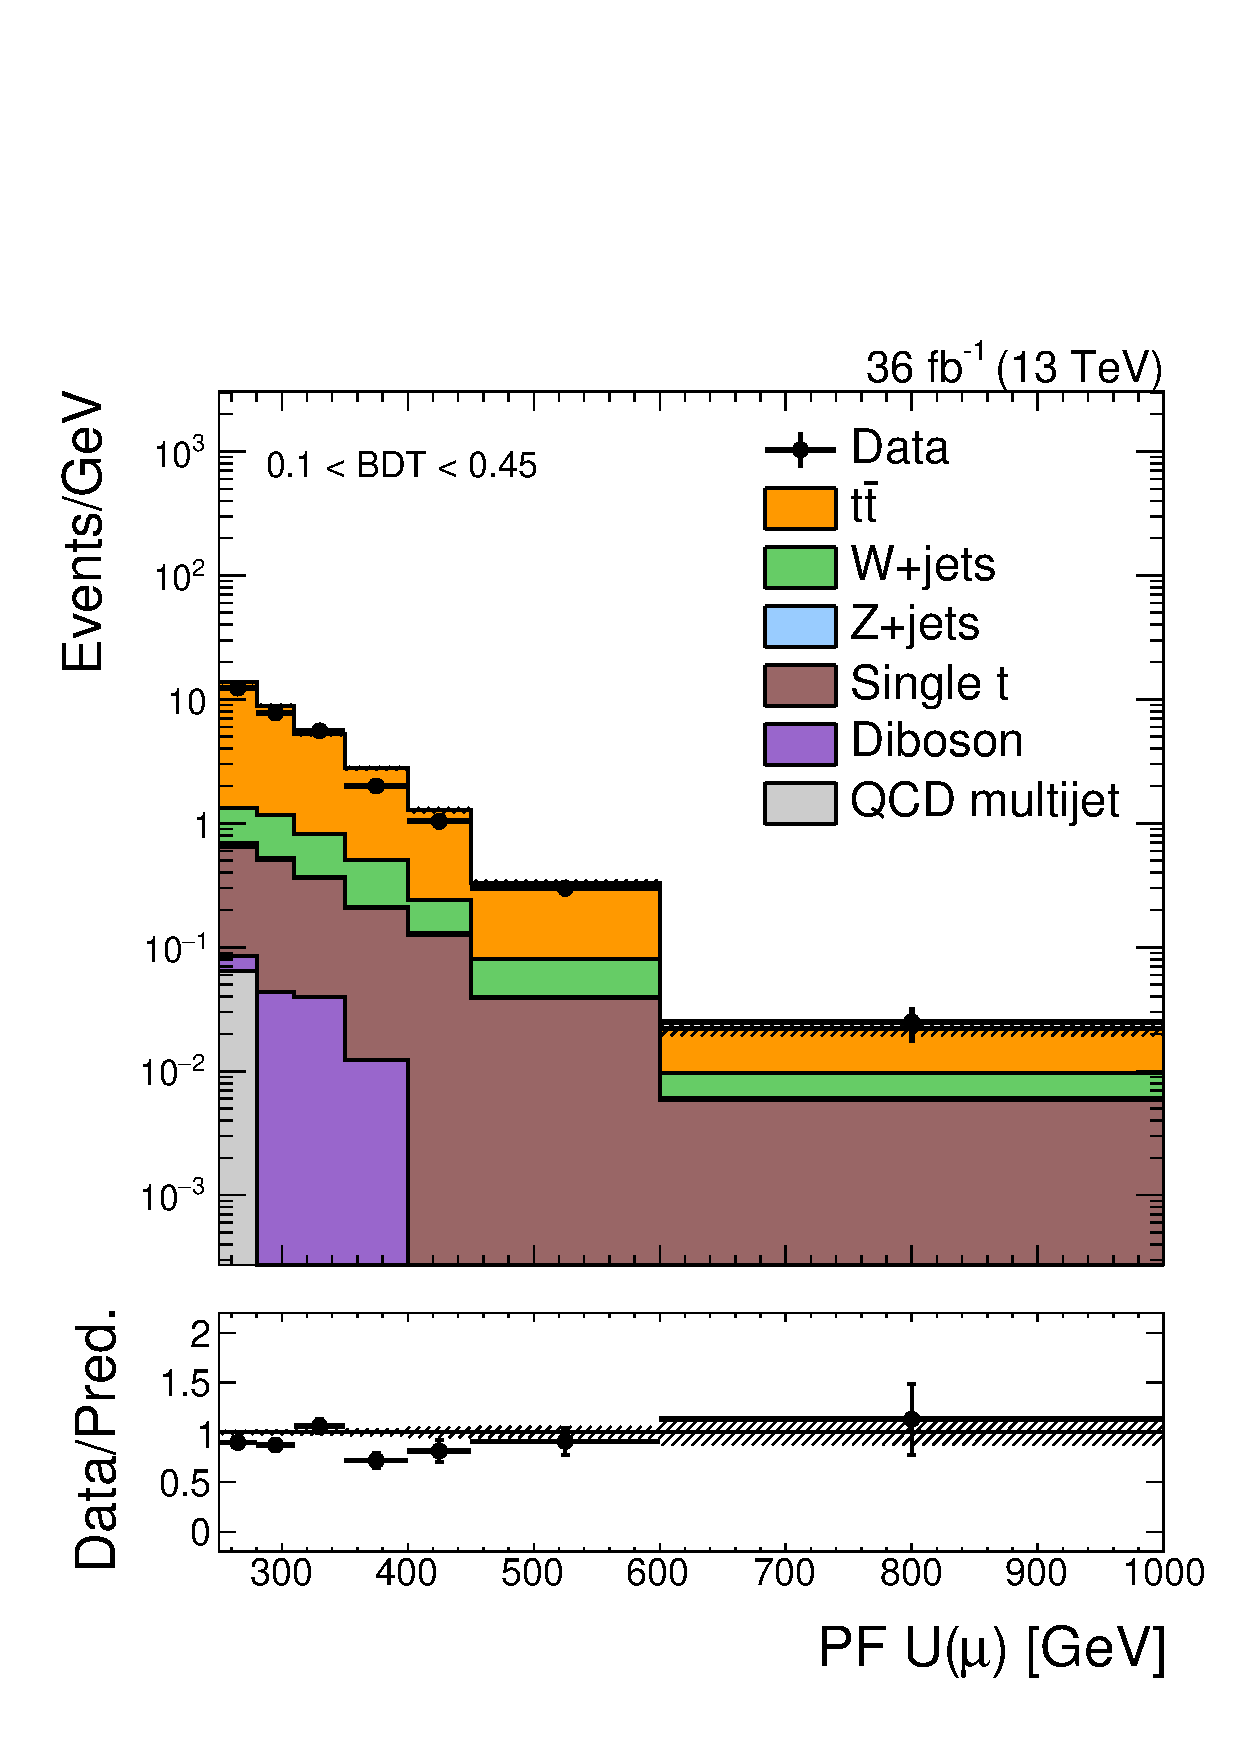
\includegraphics[width=\textwidth]{figures/monotop/prefit/singlemuontop_loose_pfUWmag_logy.pdf}
            \caption{$U$ in loose CR}
        \end{subfigure}
        \begin{subfigure}[t]{0.32\textwidth}
            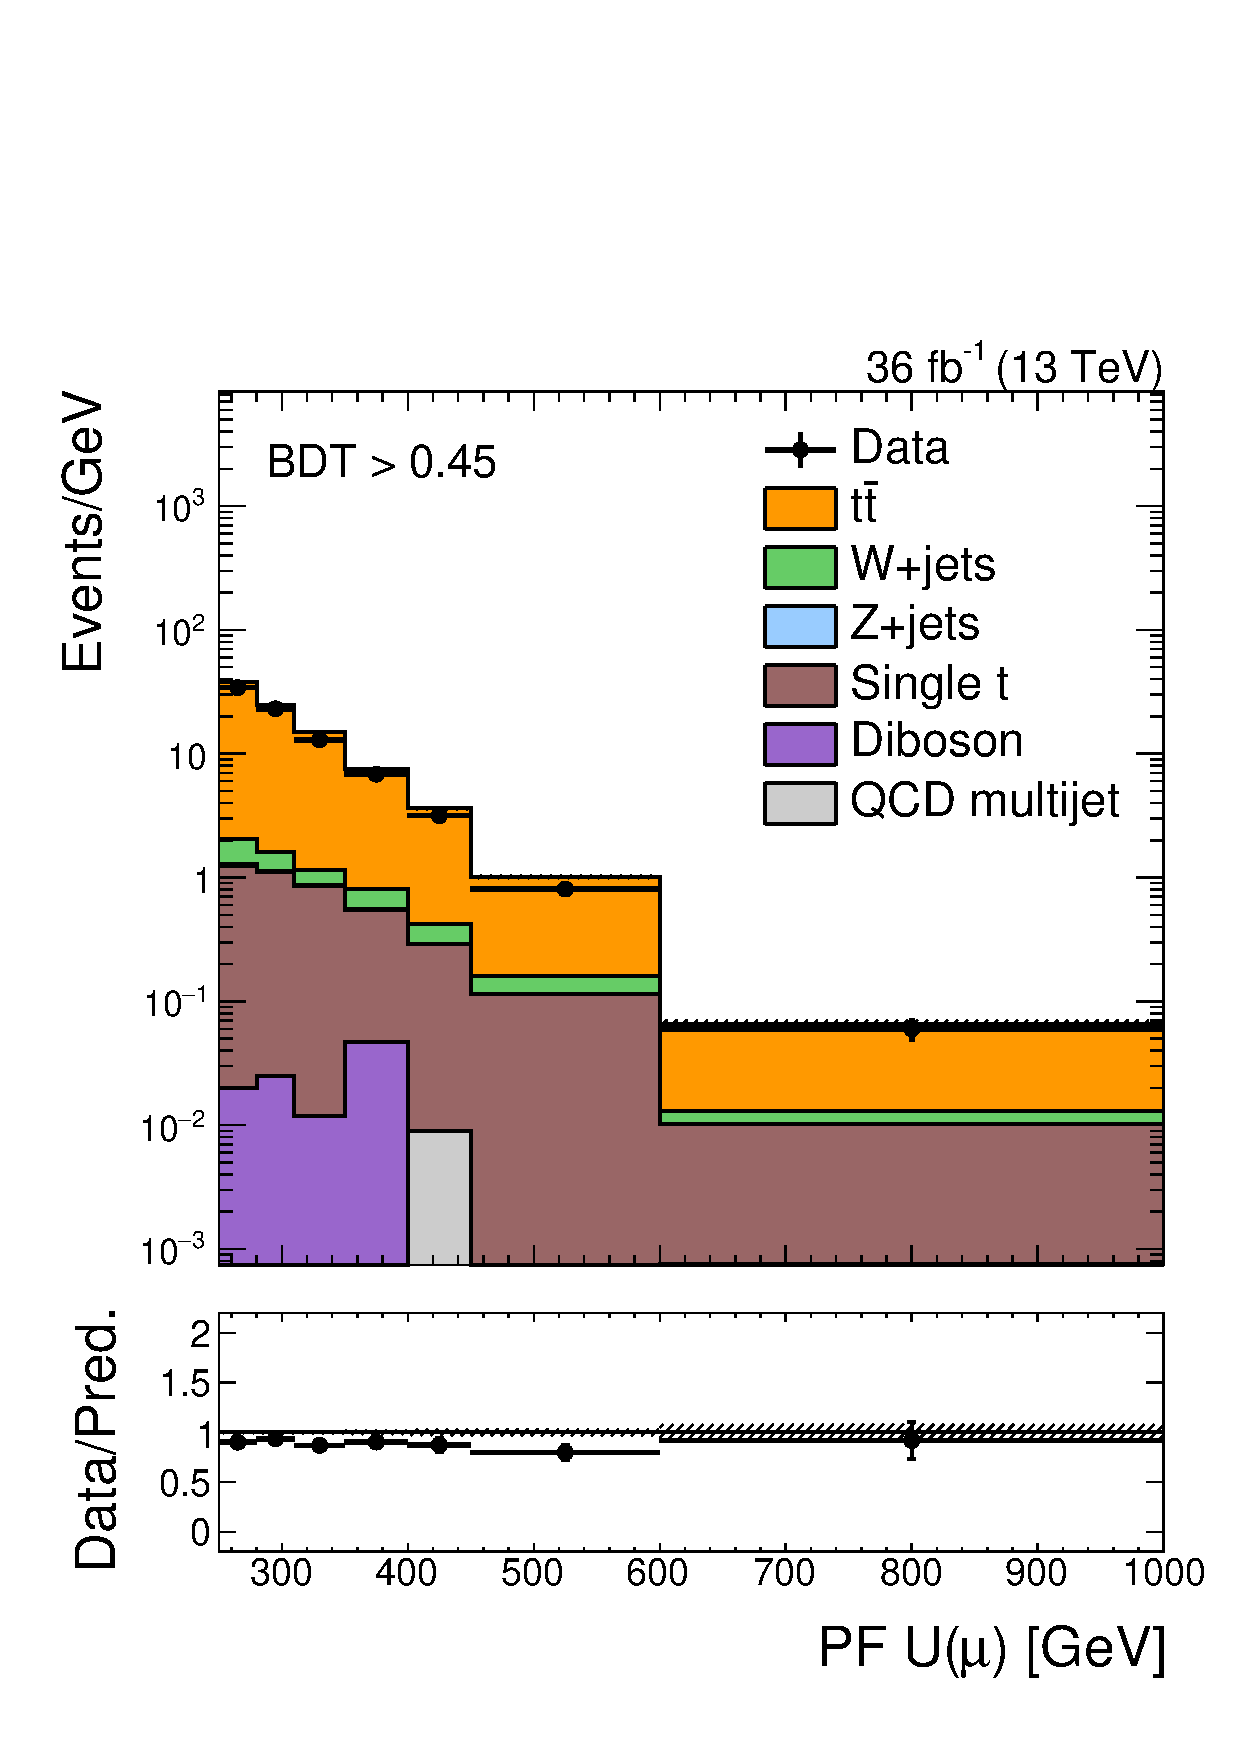
\includegraphics[width=\textwidth]{figures/monotop/prefit/singlemuontop_tight_pfUWmag_logy.pdf}
            \caption{$U$ in tight CR}
        \end{subfigure}
        \begin{subfigure}[t]{0.32\textwidth}
            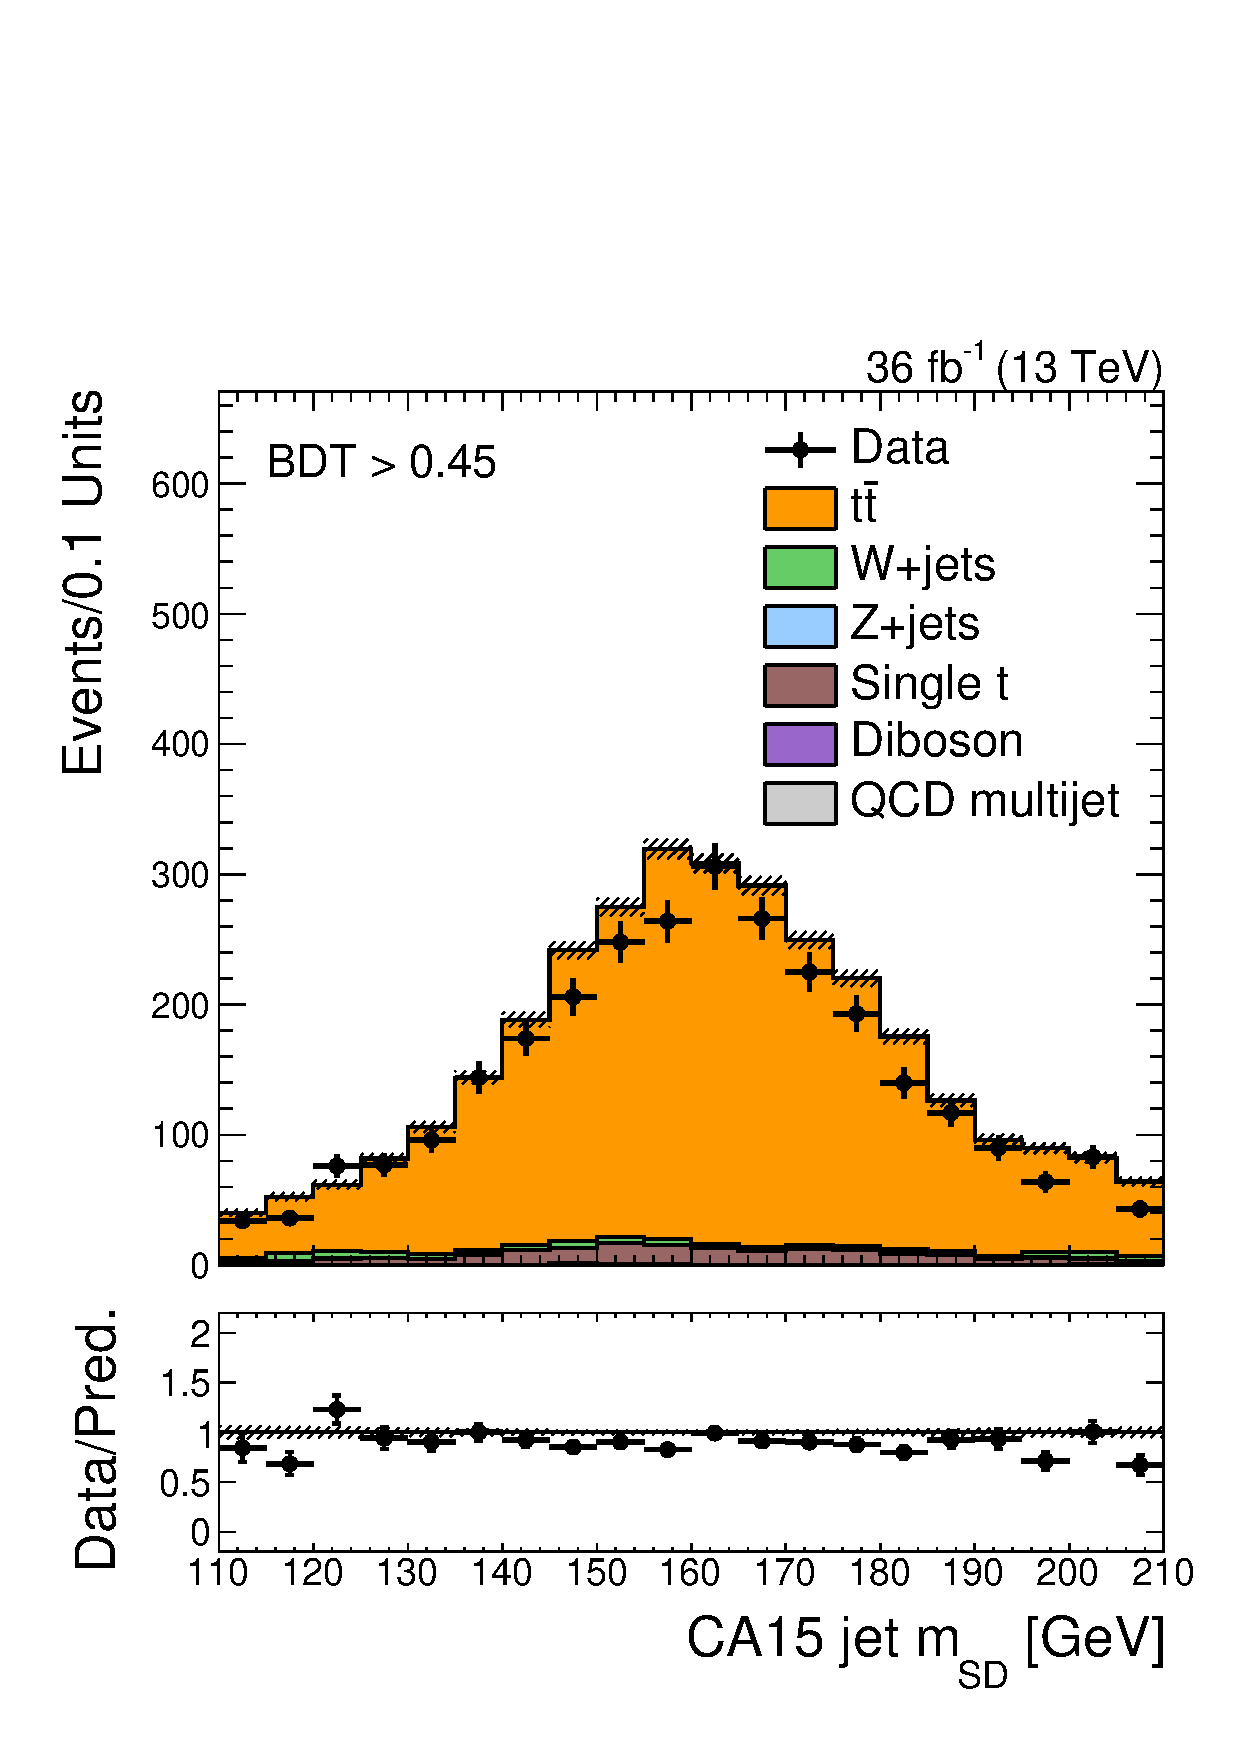
\includegraphics[width=\textwidth]{figures/monotop/prefit/singlemuontop_tight_fj1MSD.pdf}
            \caption{$m_\mathrm{SD}$}
        \end{subfigure}
        \caption{Various kinematic distributions in the two mono-top $b\mu$ CRs. }
        \label{fig:mt:prefit_tmn}
    \end{center}
\end{figure}

\begin{figure}[]
    \begin{center}
        \begin{subfigure}[t]{0.32\textwidth}
            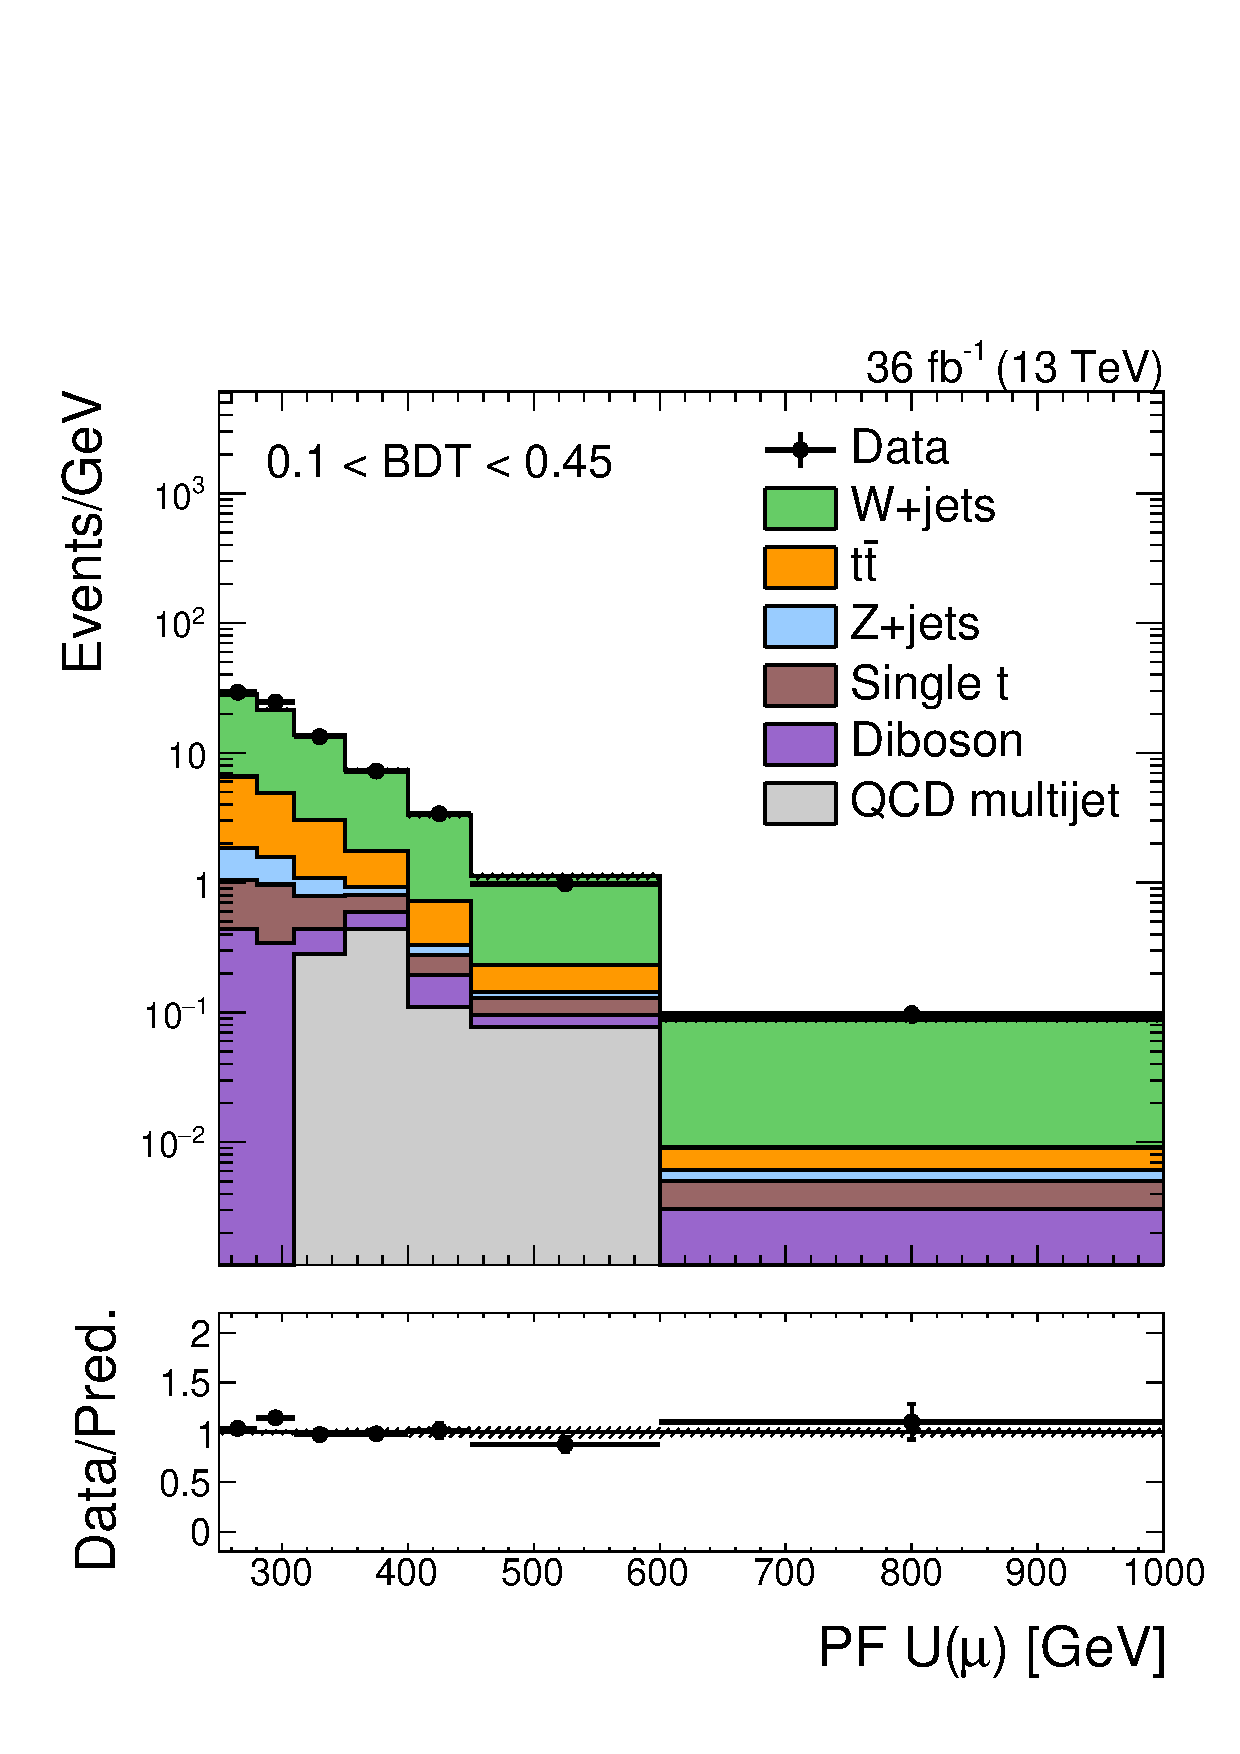
\includegraphics[width=\textwidth]{figures/monotop/prefit/singlemuonw_loose_pfUWmag_logy.pdf}
            \caption{$U$ in loose CR}
        \end{subfigure}
        \begin{subfigure}[t]{0.32\textwidth}
            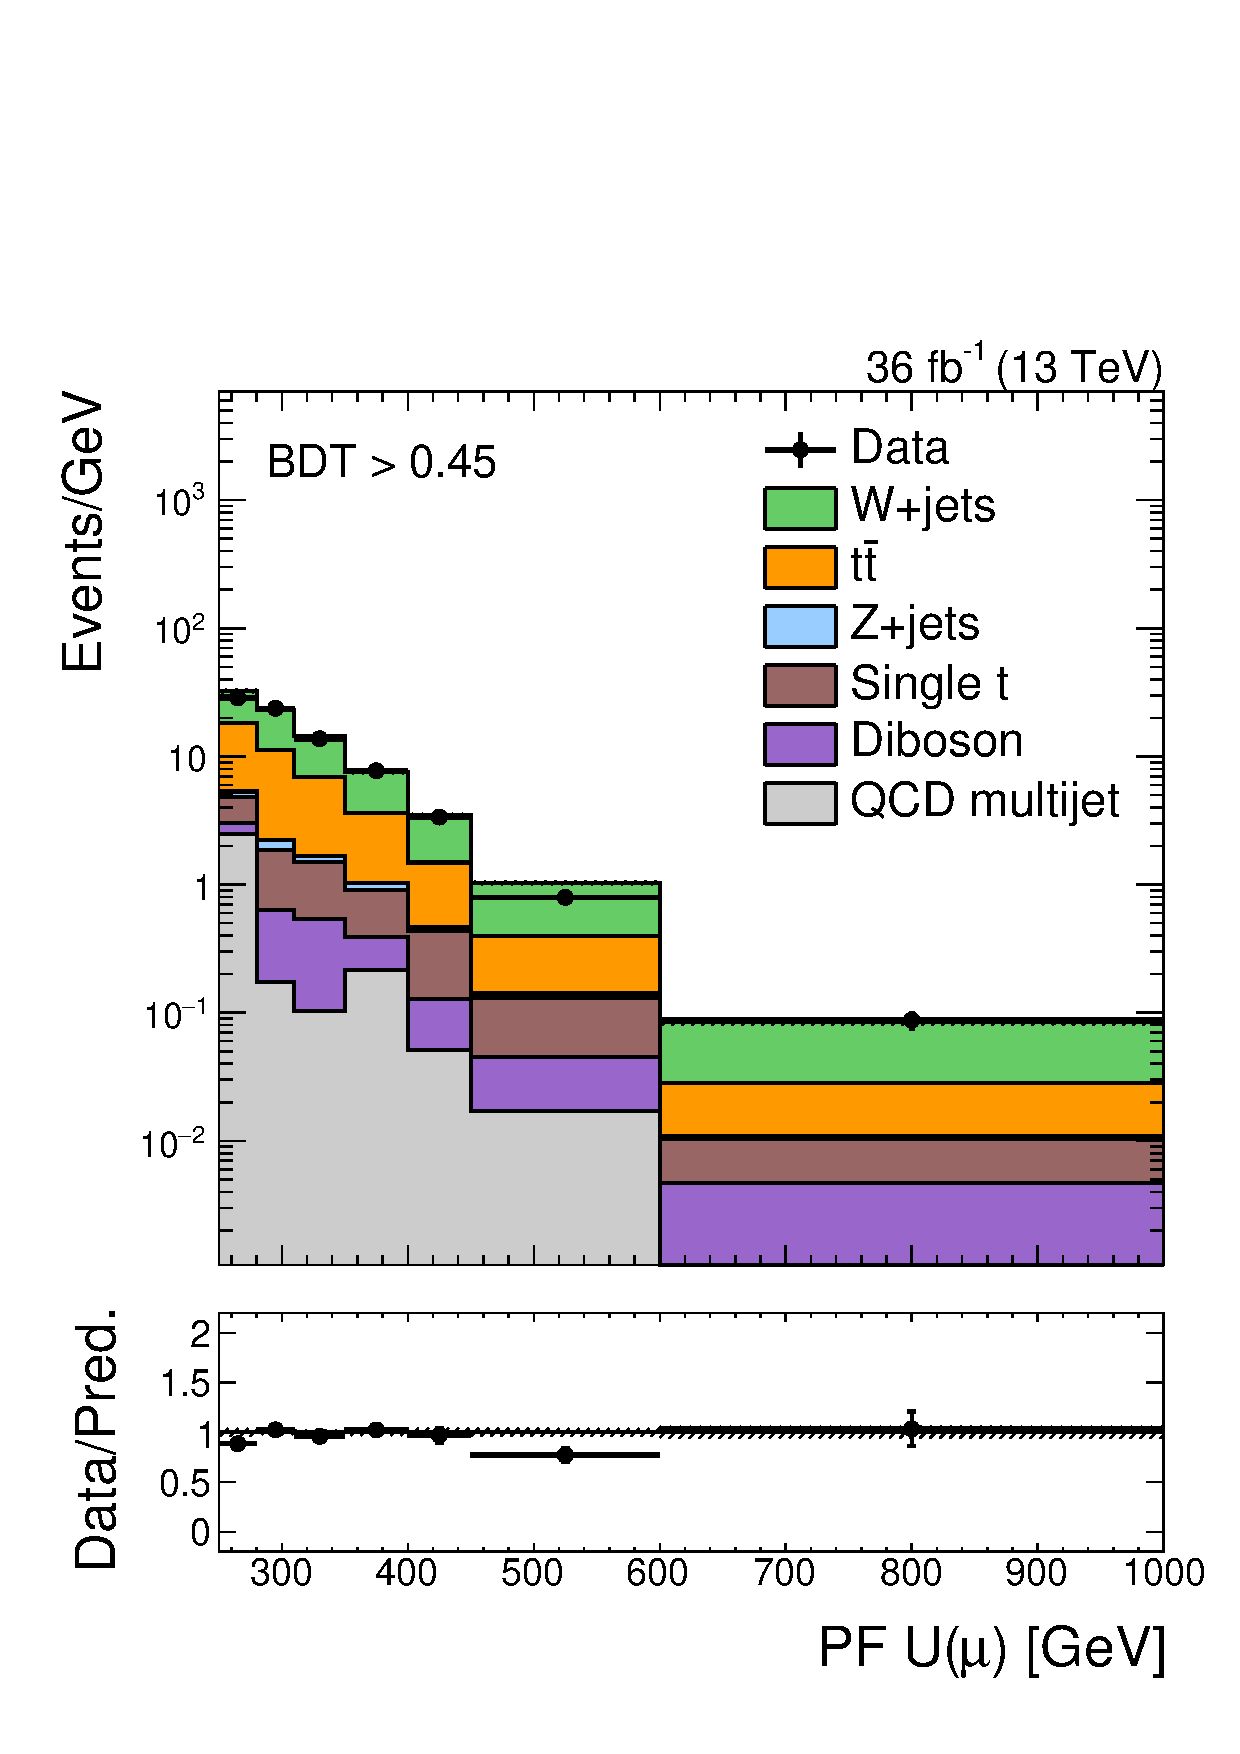
\includegraphics[width=\textwidth]{figures/monotop/prefit/singlemuonw_tight_pfUWmag_logy.pdf}
            \caption{$U$ in tight CR}
            \label{fig:mt:prefit_wmn:tight1}
        \end{subfigure}
        \begin{subfigure}[t]{0.32\textwidth}
            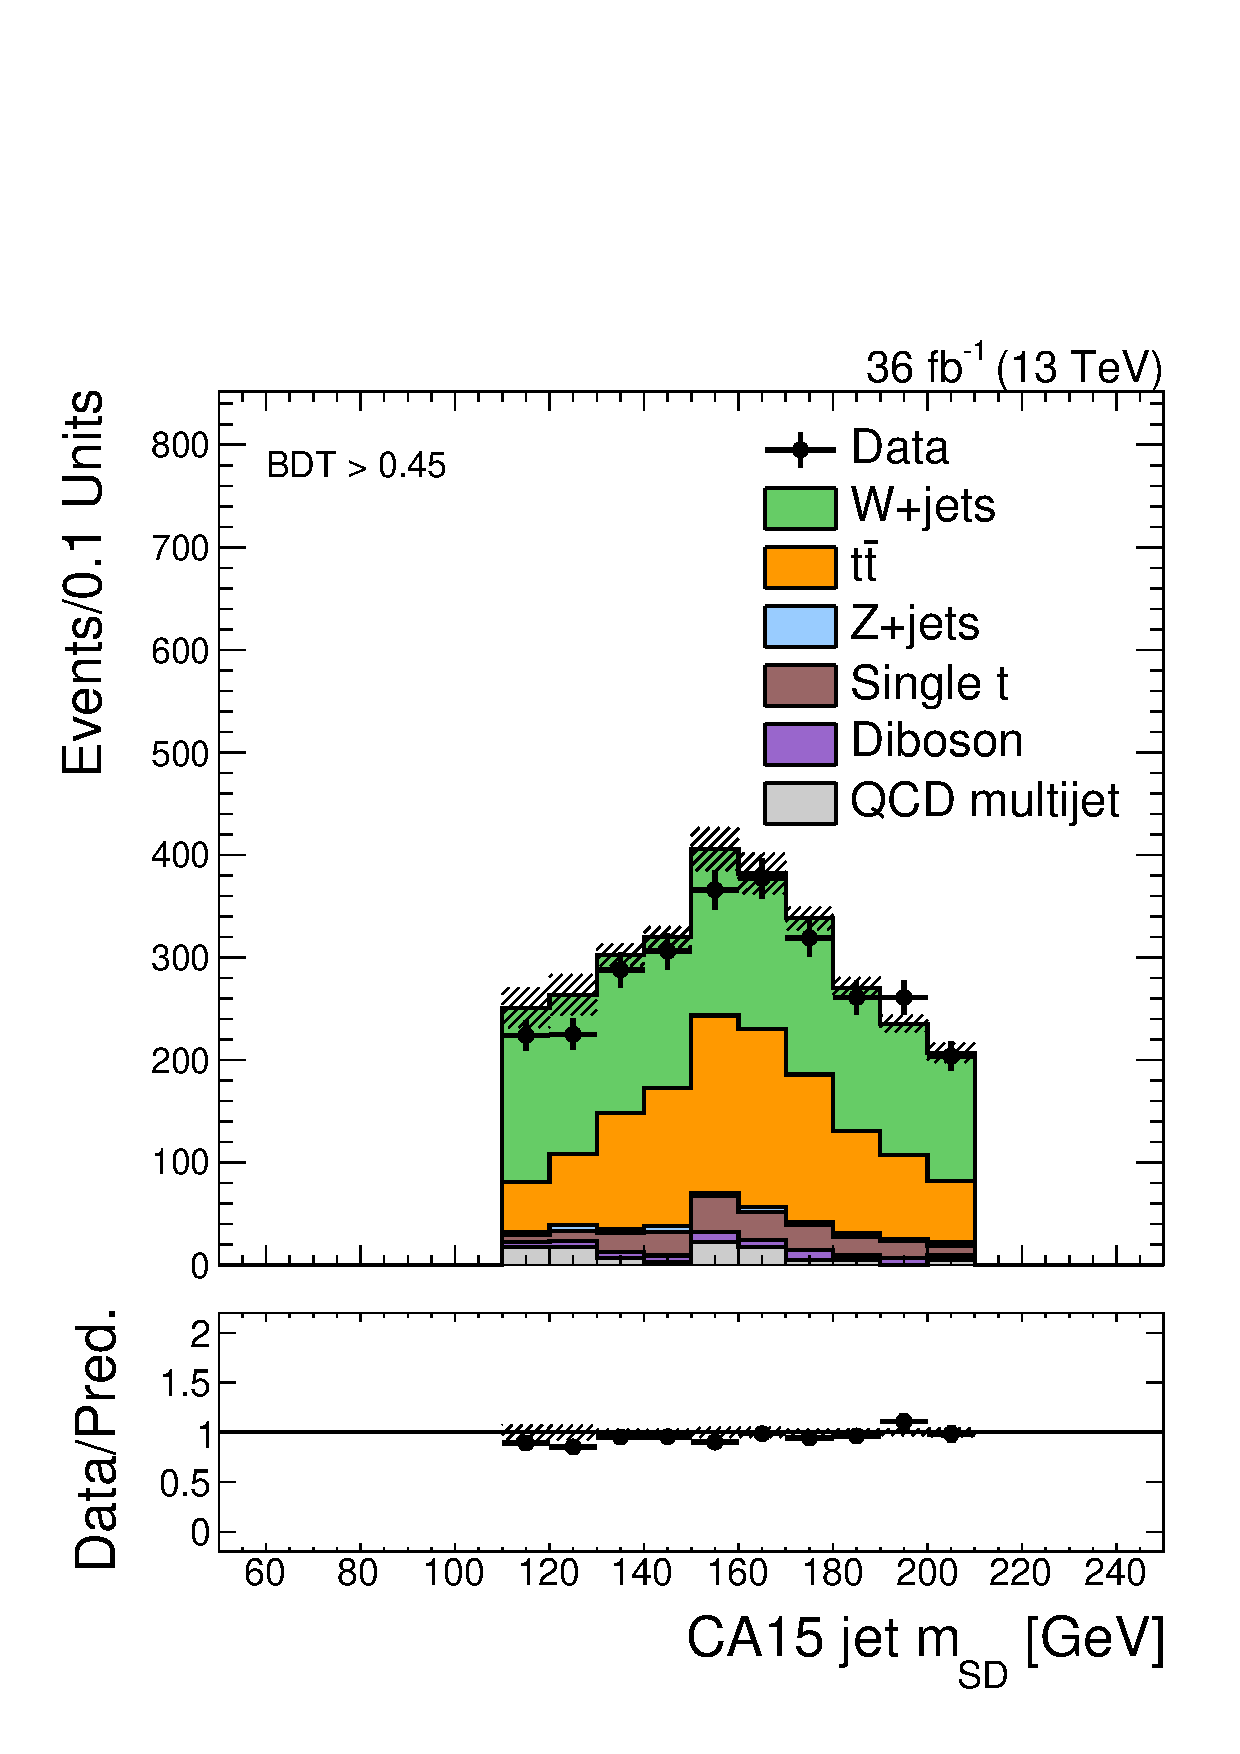
\includegraphics[width=\textwidth]{figures/monotop/prefit/singlemuonw_tight_fj1MSD.pdf}
            \caption{$m_\mathrm{SD}$}
            \label{fig:mt:prefit_wmn:tight2}
        \end{subfigure}
        \caption{Various kinematic distributions in the two mono-top $\mu$ CRs. }
        \label{fig:mt:prefit_wmn}
    \end{center}
\end{figure}

Each CR gets a set of transfer factors to constrain the targetted process in the SR: $\T{b\mu}{t\bar{t}}$ and $\T{\mu}{W}$. 
In the tight $\mu$ CR (Figures \ref{fig:mt:prefit_wmn:tight1}-\ref{fig:mt:prefit_wmn:tight2}), the stringent top ID requirement enhances the $t\bar{t}$ and suppresses the $W$ contribution. 
Since we cannot create a pure $W$ in the tight category, we introduce an additional set of transfer factors $\T{\mu}{t\bar{t}}$. 
This extra constraint uses the $b\mu$ CRs to estimate the $t\bar{t}$ component in the $\mu$ CRs, thereby leaving only one large degree of freedom in the $\mu$ CRs.
These three sets of transfer factors, and the corresponding uncertainties, are shown in Figure~\ref{fig:mt:mn_xfer}. 


\begin{figure}[]
    \begin{center}
        \begin{subfigure}[t]{0.49\textwidth}
            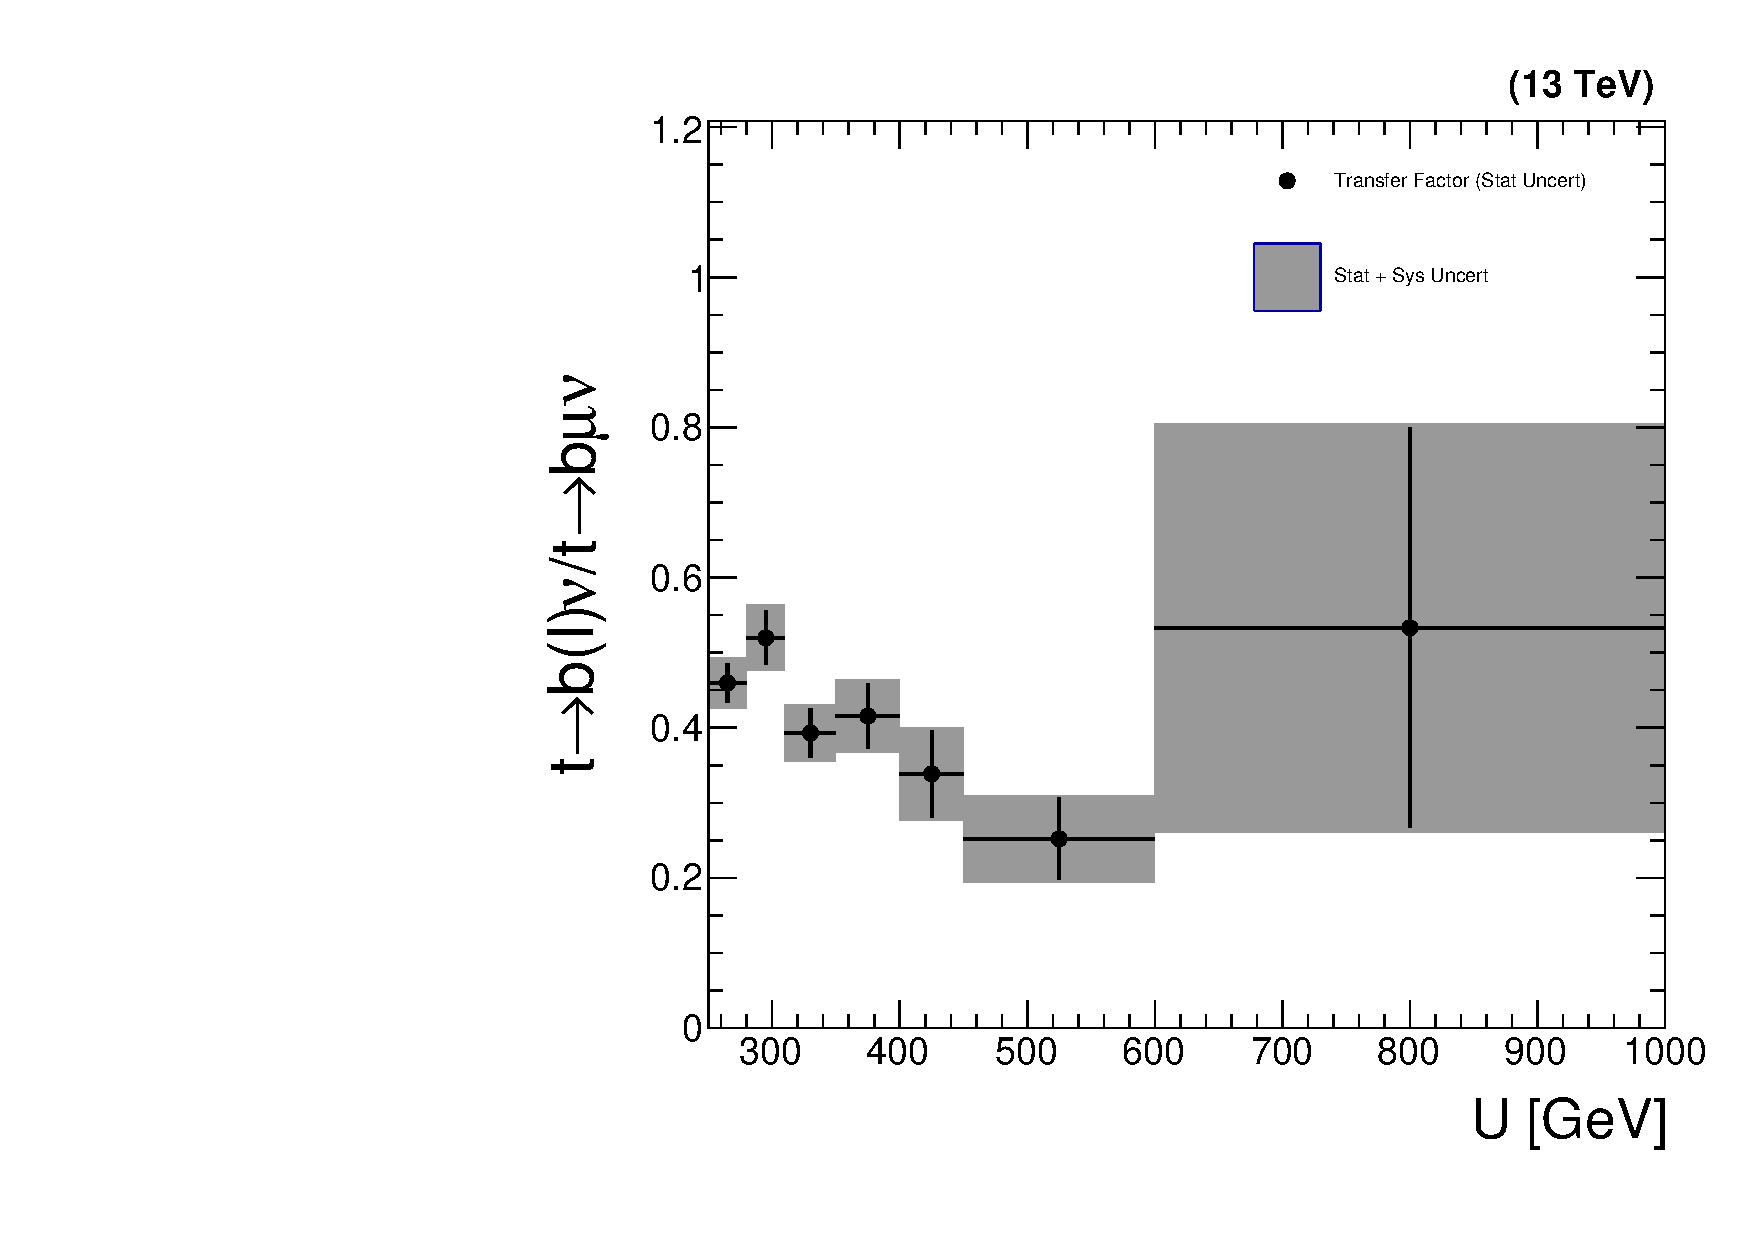
\includegraphics[width=0.49\textwidth]{figures/monotop/xfer/rfactor_singlemuontop_loose.pdf}
            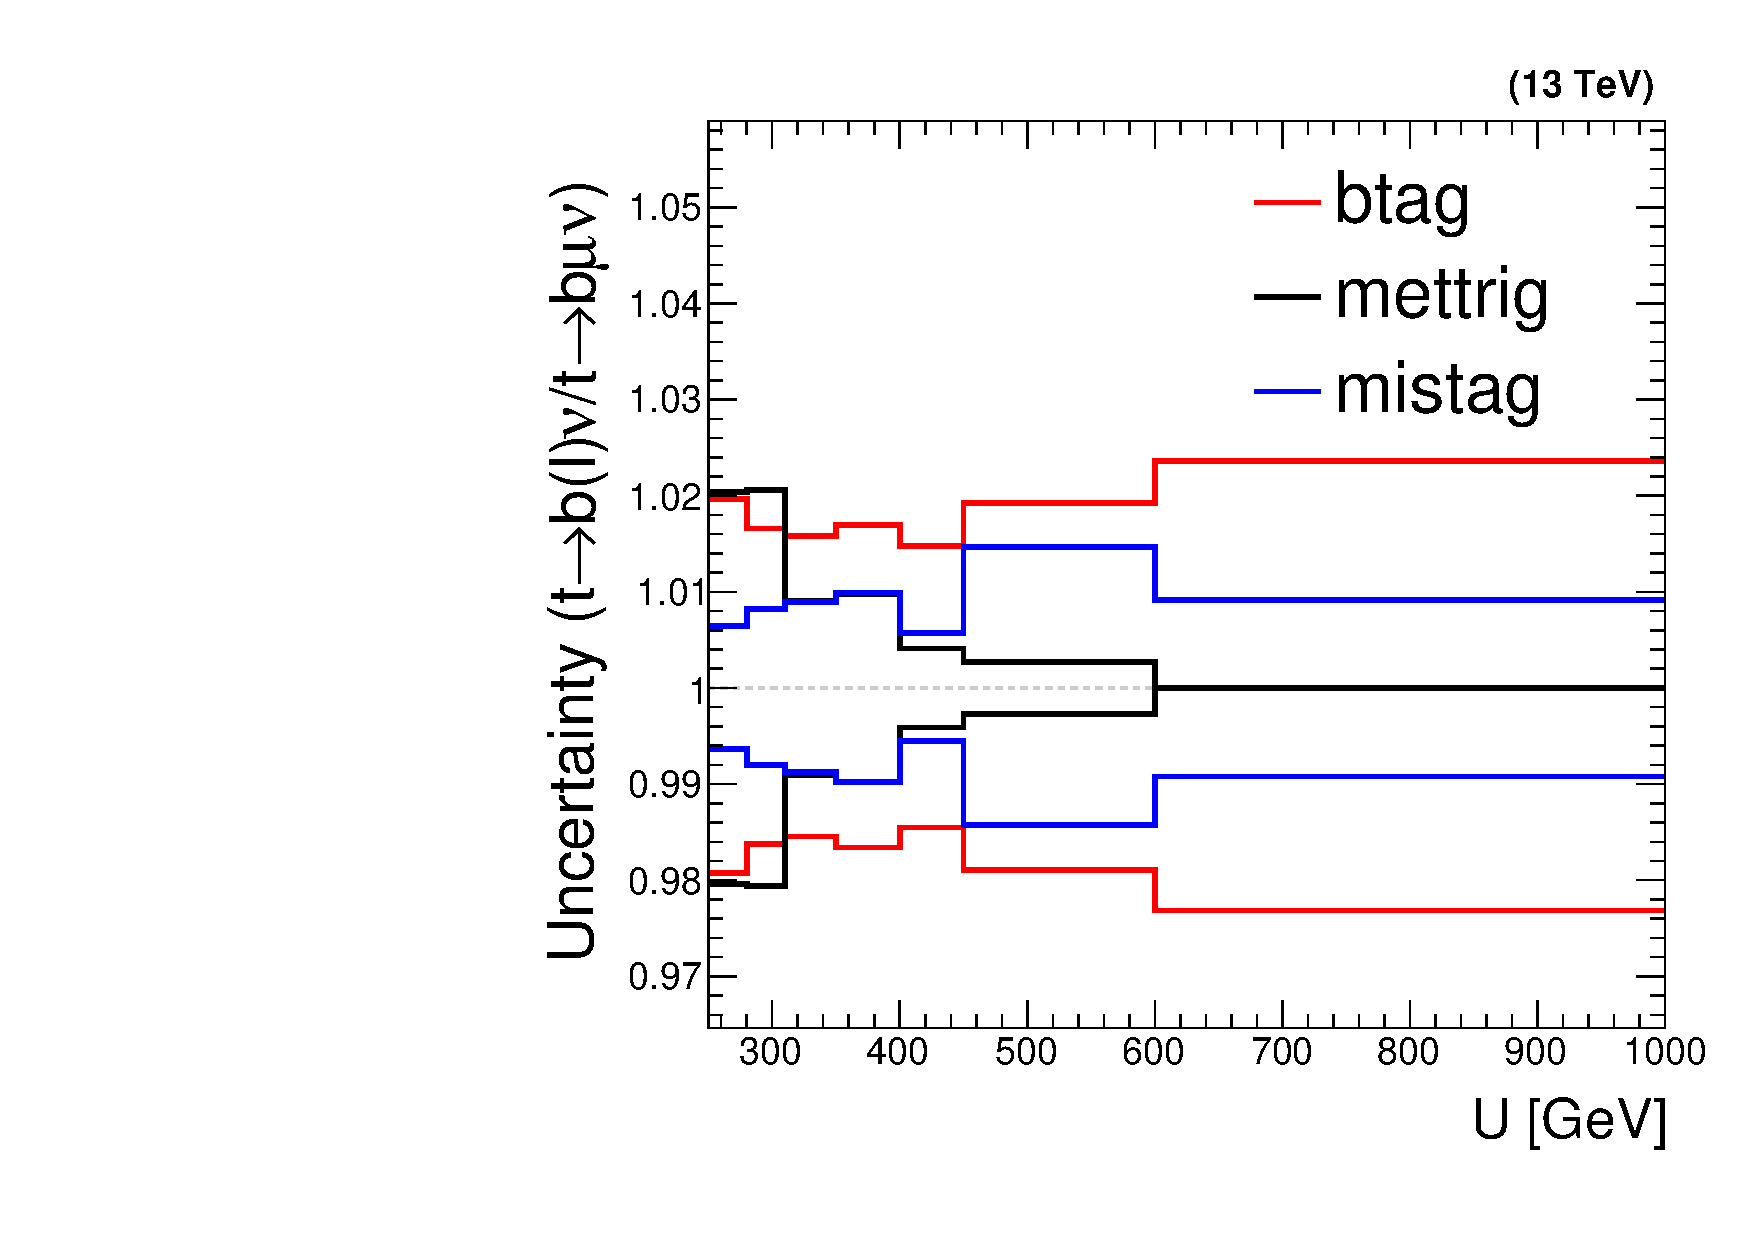
\includegraphics[width=0.49\textwidth]{figures/monotop/uncertainties/variations_singlemuontop_loose.pdf}
            \caption{Loose $\T{b\mu}{t\bar{t}}$}
        \end{subfigure}
        \begin{subfigure}[t]{0.49\textwidth}
            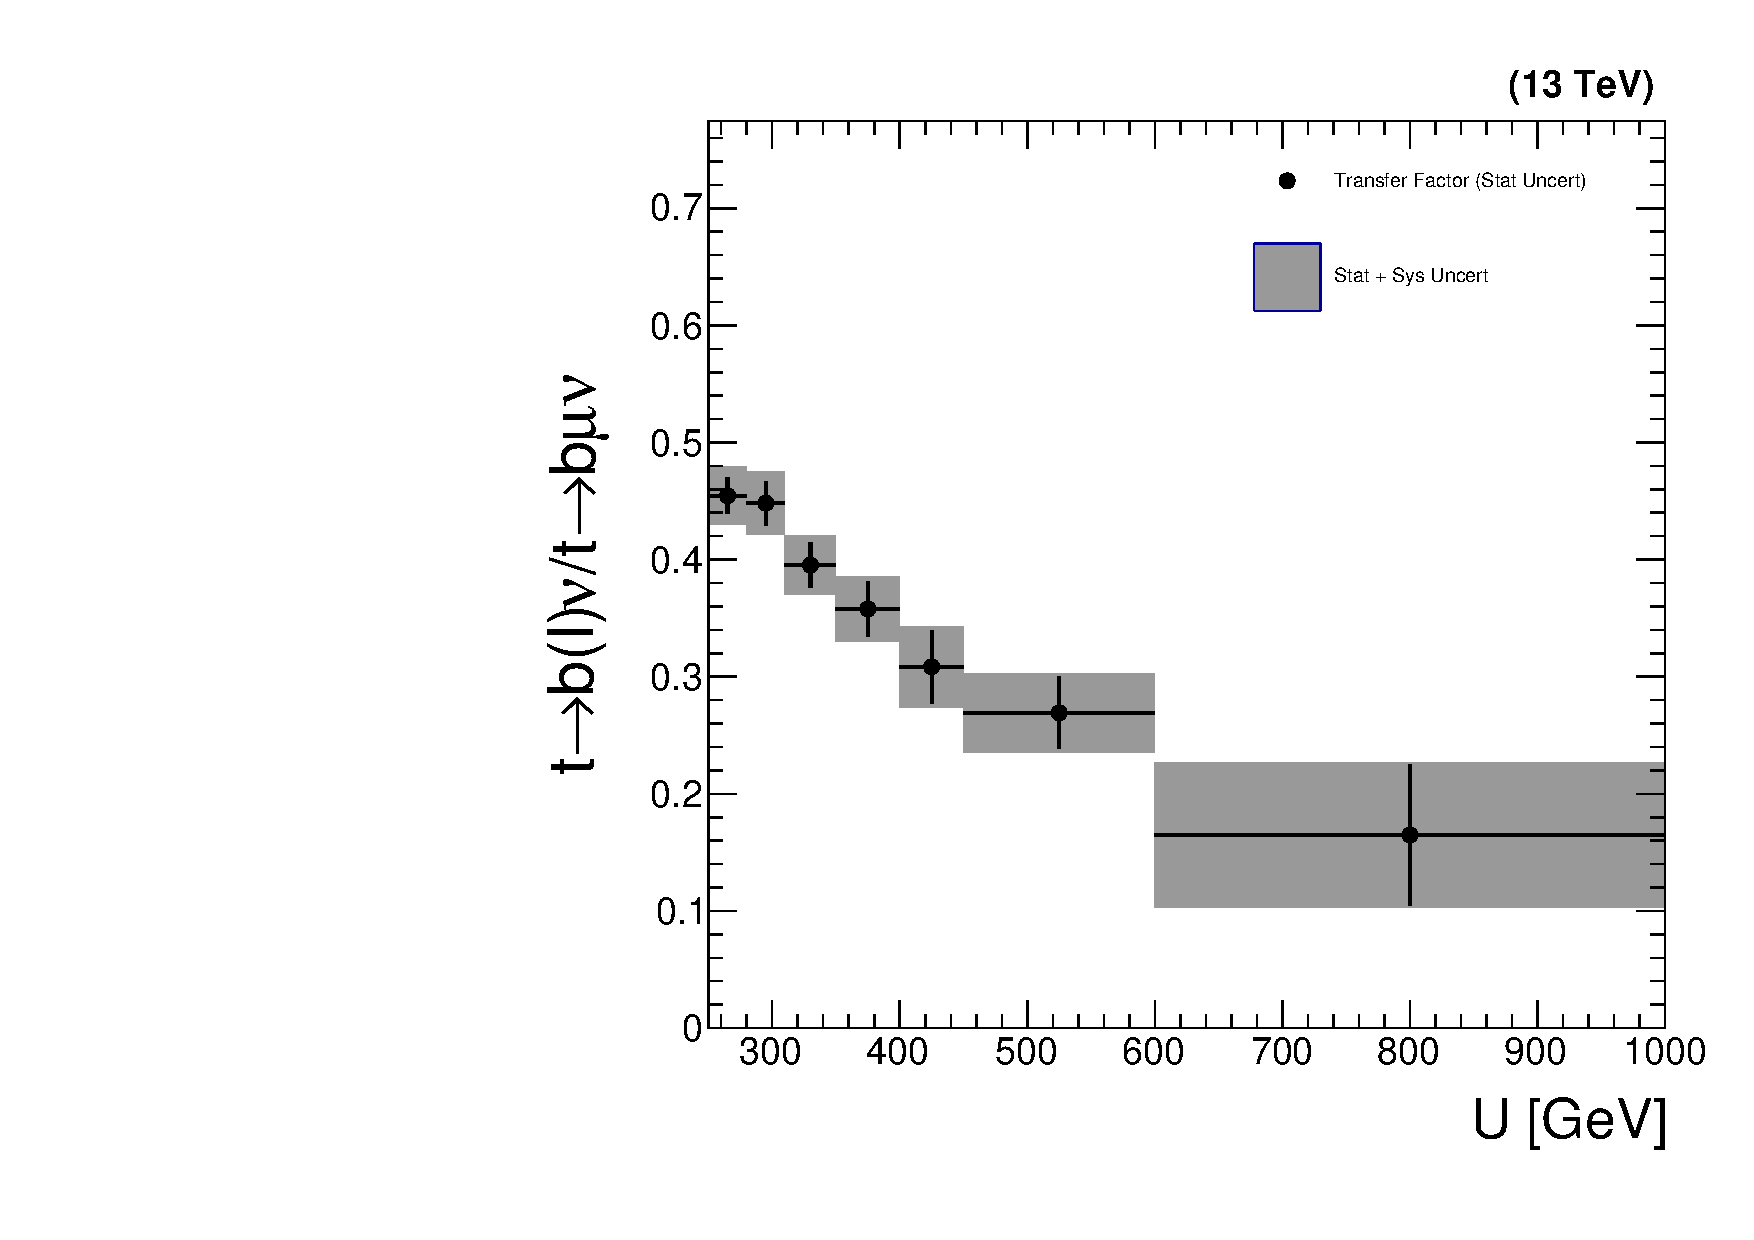
\includegraphics[width=0.49\textwidth]{figures/monotop/xfer/rfactor_singlemuontop.pdf}
            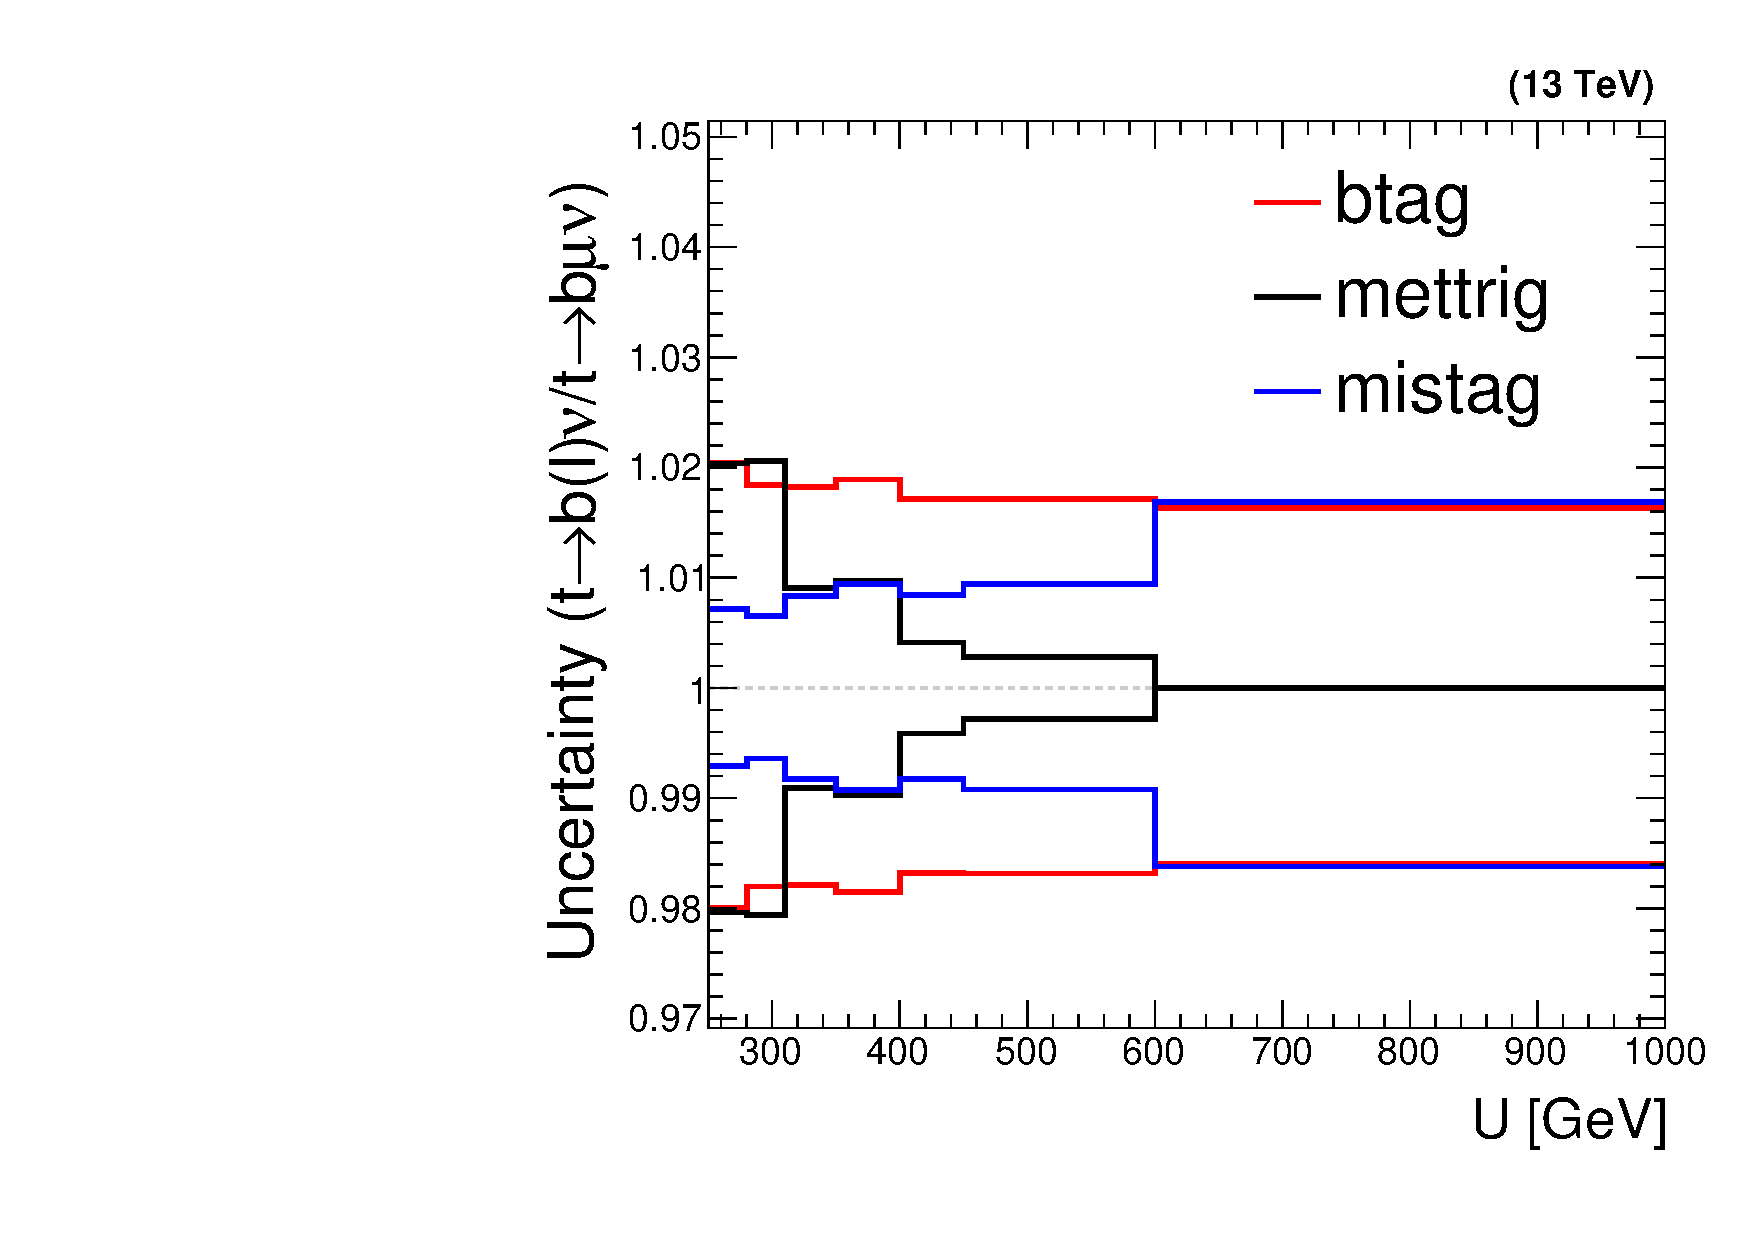
\includegraphics[width=0.49\textwidth]{figures/monotop/uncertainties/variations_singlemuontop.pdf}
            \caption{Tight $\T{b\mu}{t\bar{t}}$}
        \end{subfigure}
        \begin{subfigure}[t]{0.49\textwidth}
            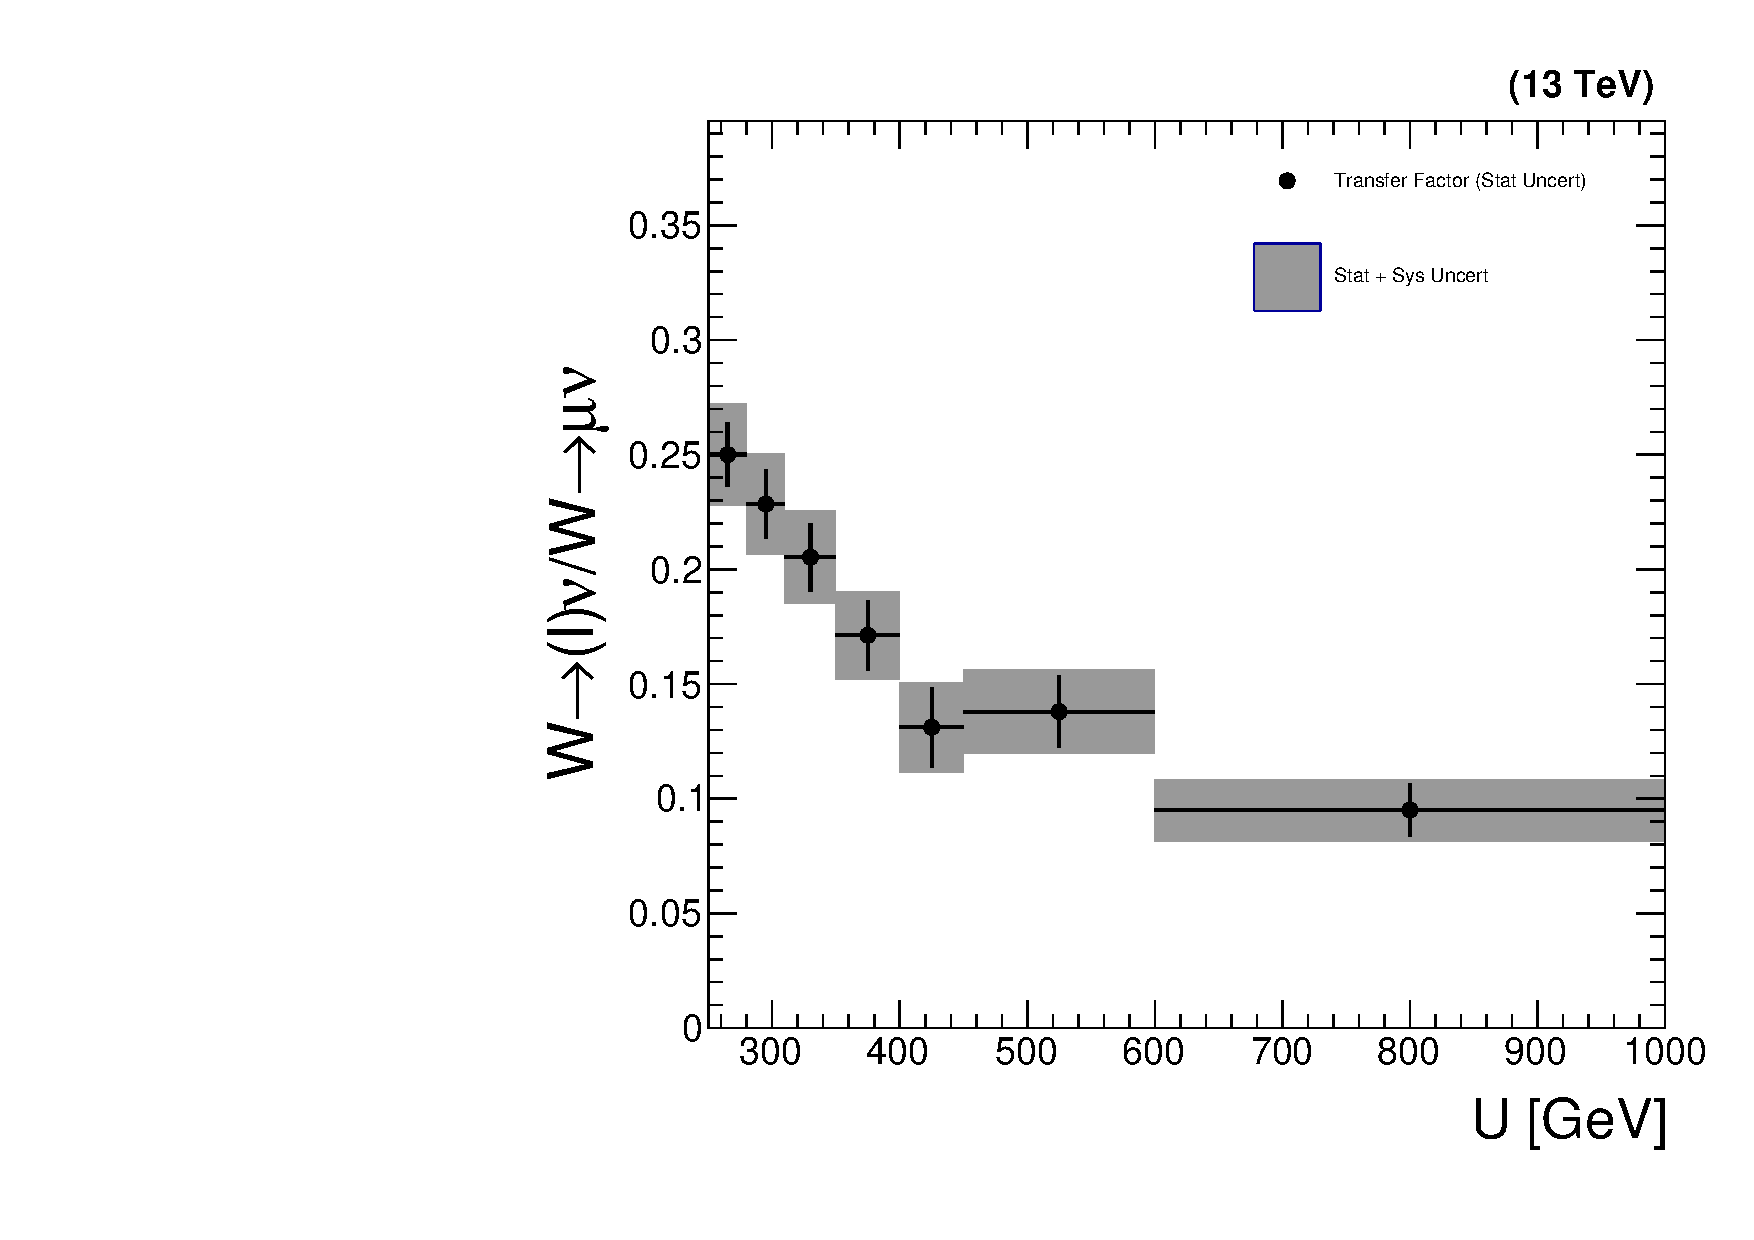
\includegraphics[width=0.49\textwidth]{figures/monotop/xfer/rfactor_singlemuonw_loose.pdf}
            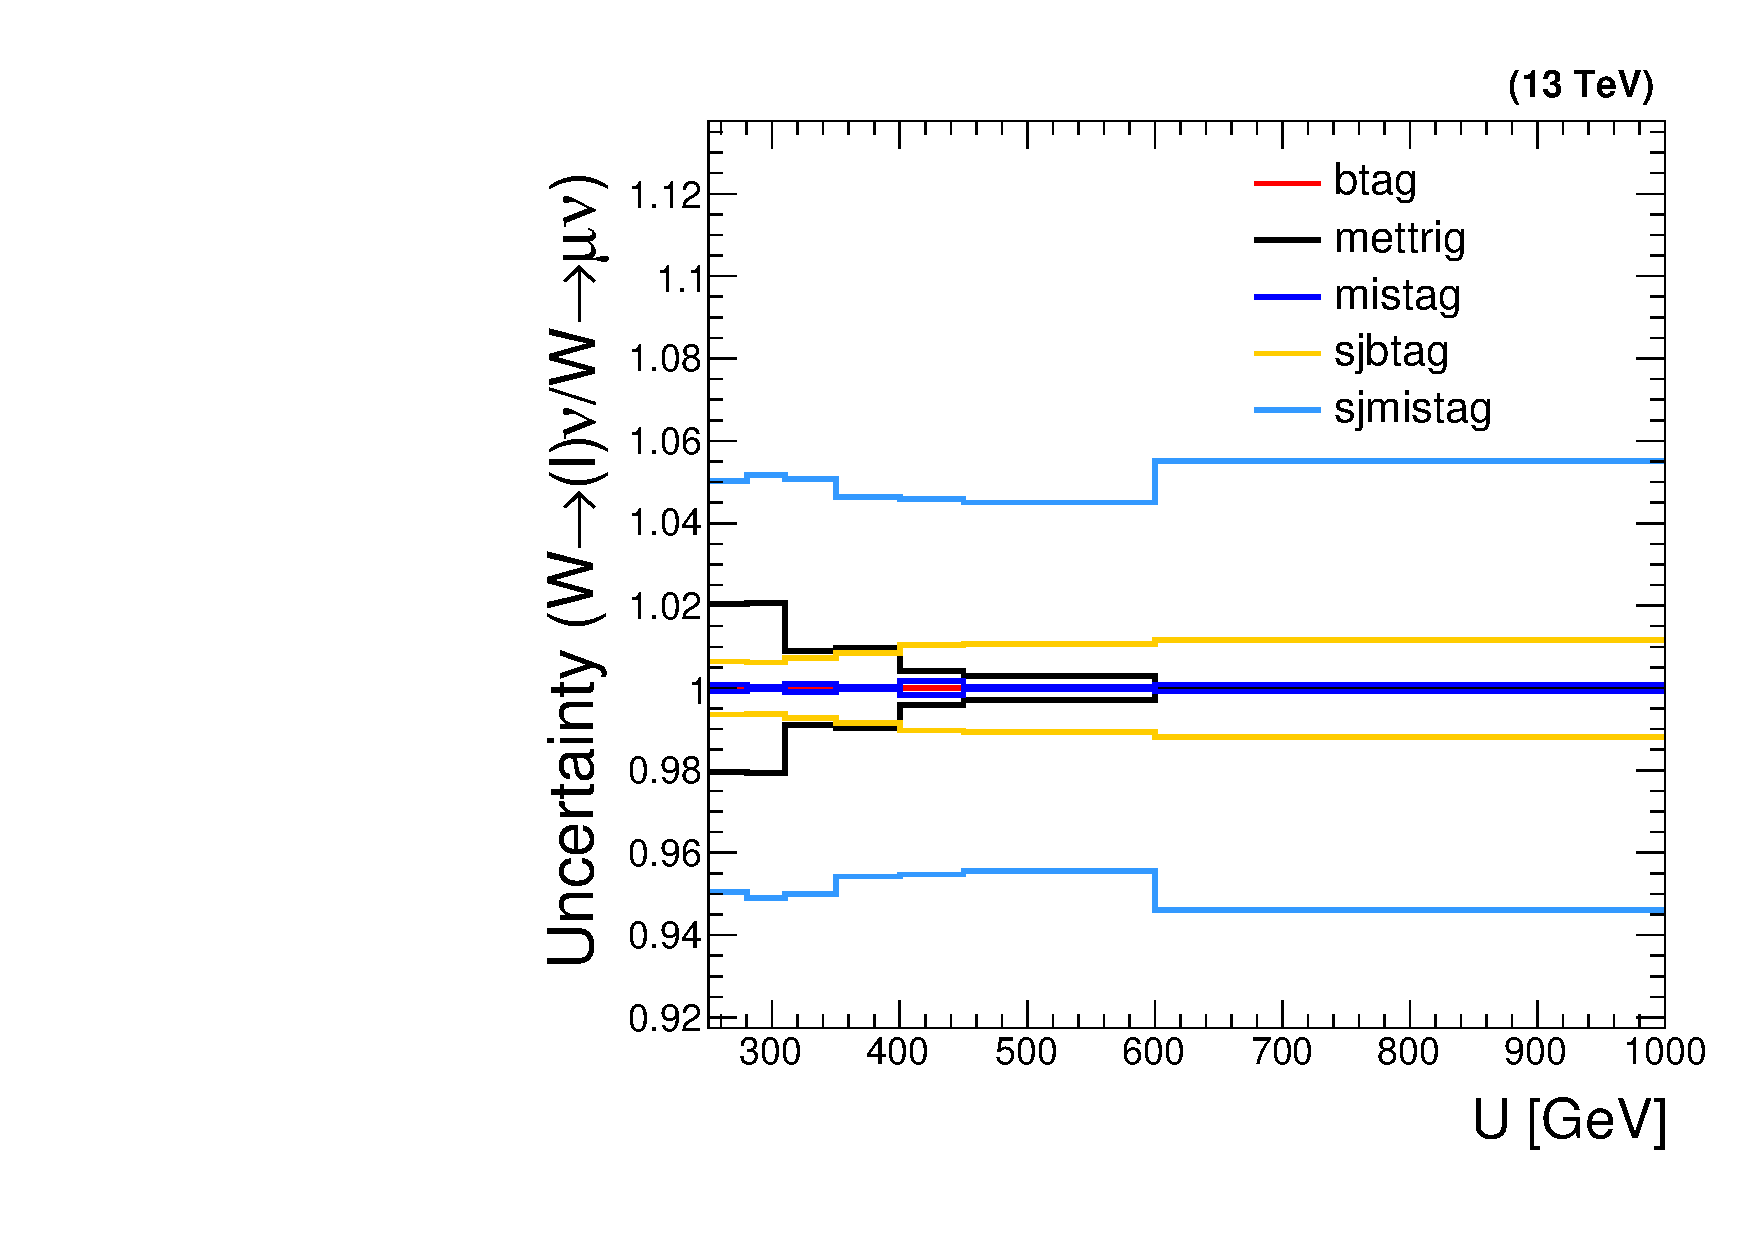
\includegraphics[width=0.49\textwidth]{figures/monotop/uncertainties/variations_singlemuonw_loose.pdf}
            \caption{Loose $\T{\mu}{W}$}
        \end{subfigure}
        \begin{subfigure}[t]{0.49\textwidth}
            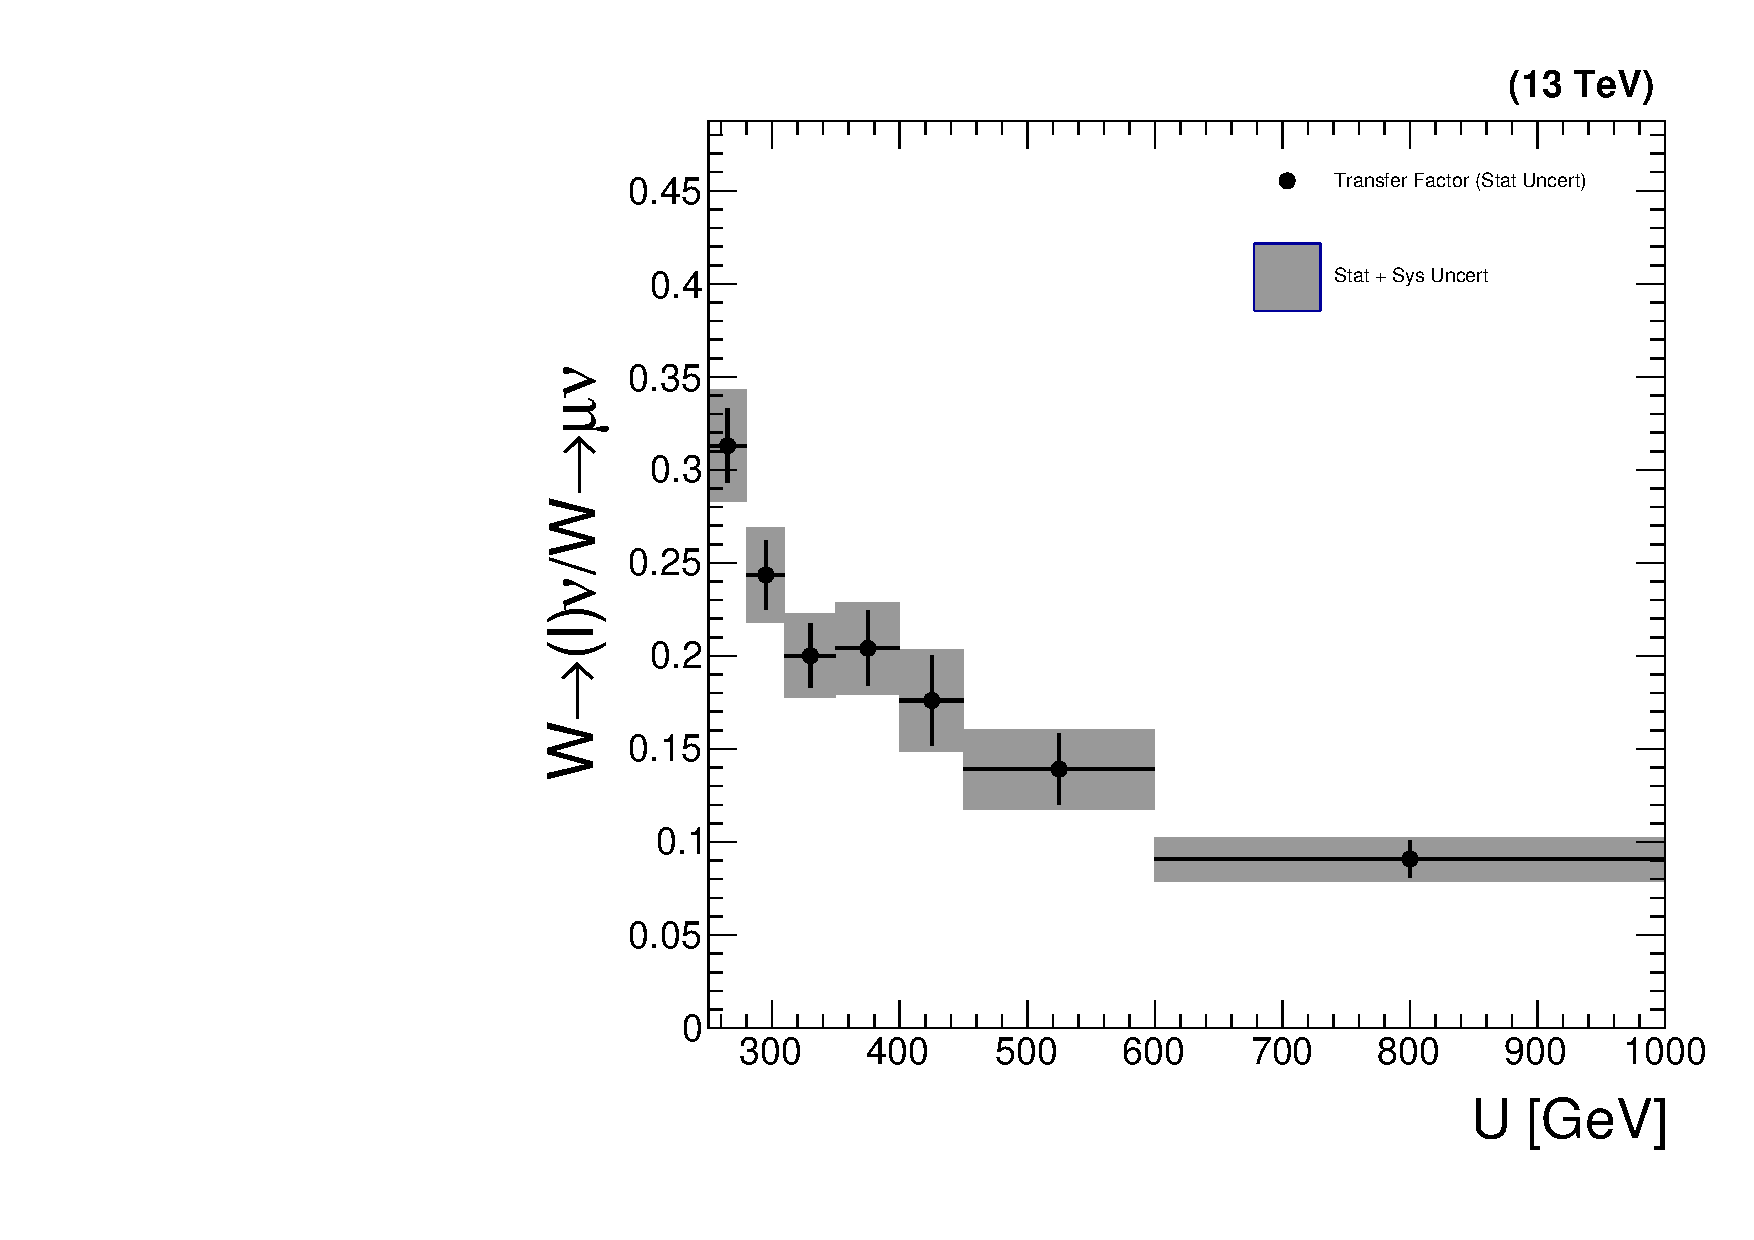
\includegraphics[width=0.49\textwidth]{figures/monotop/xfer/rfactor_singlemuonw.pdf}
            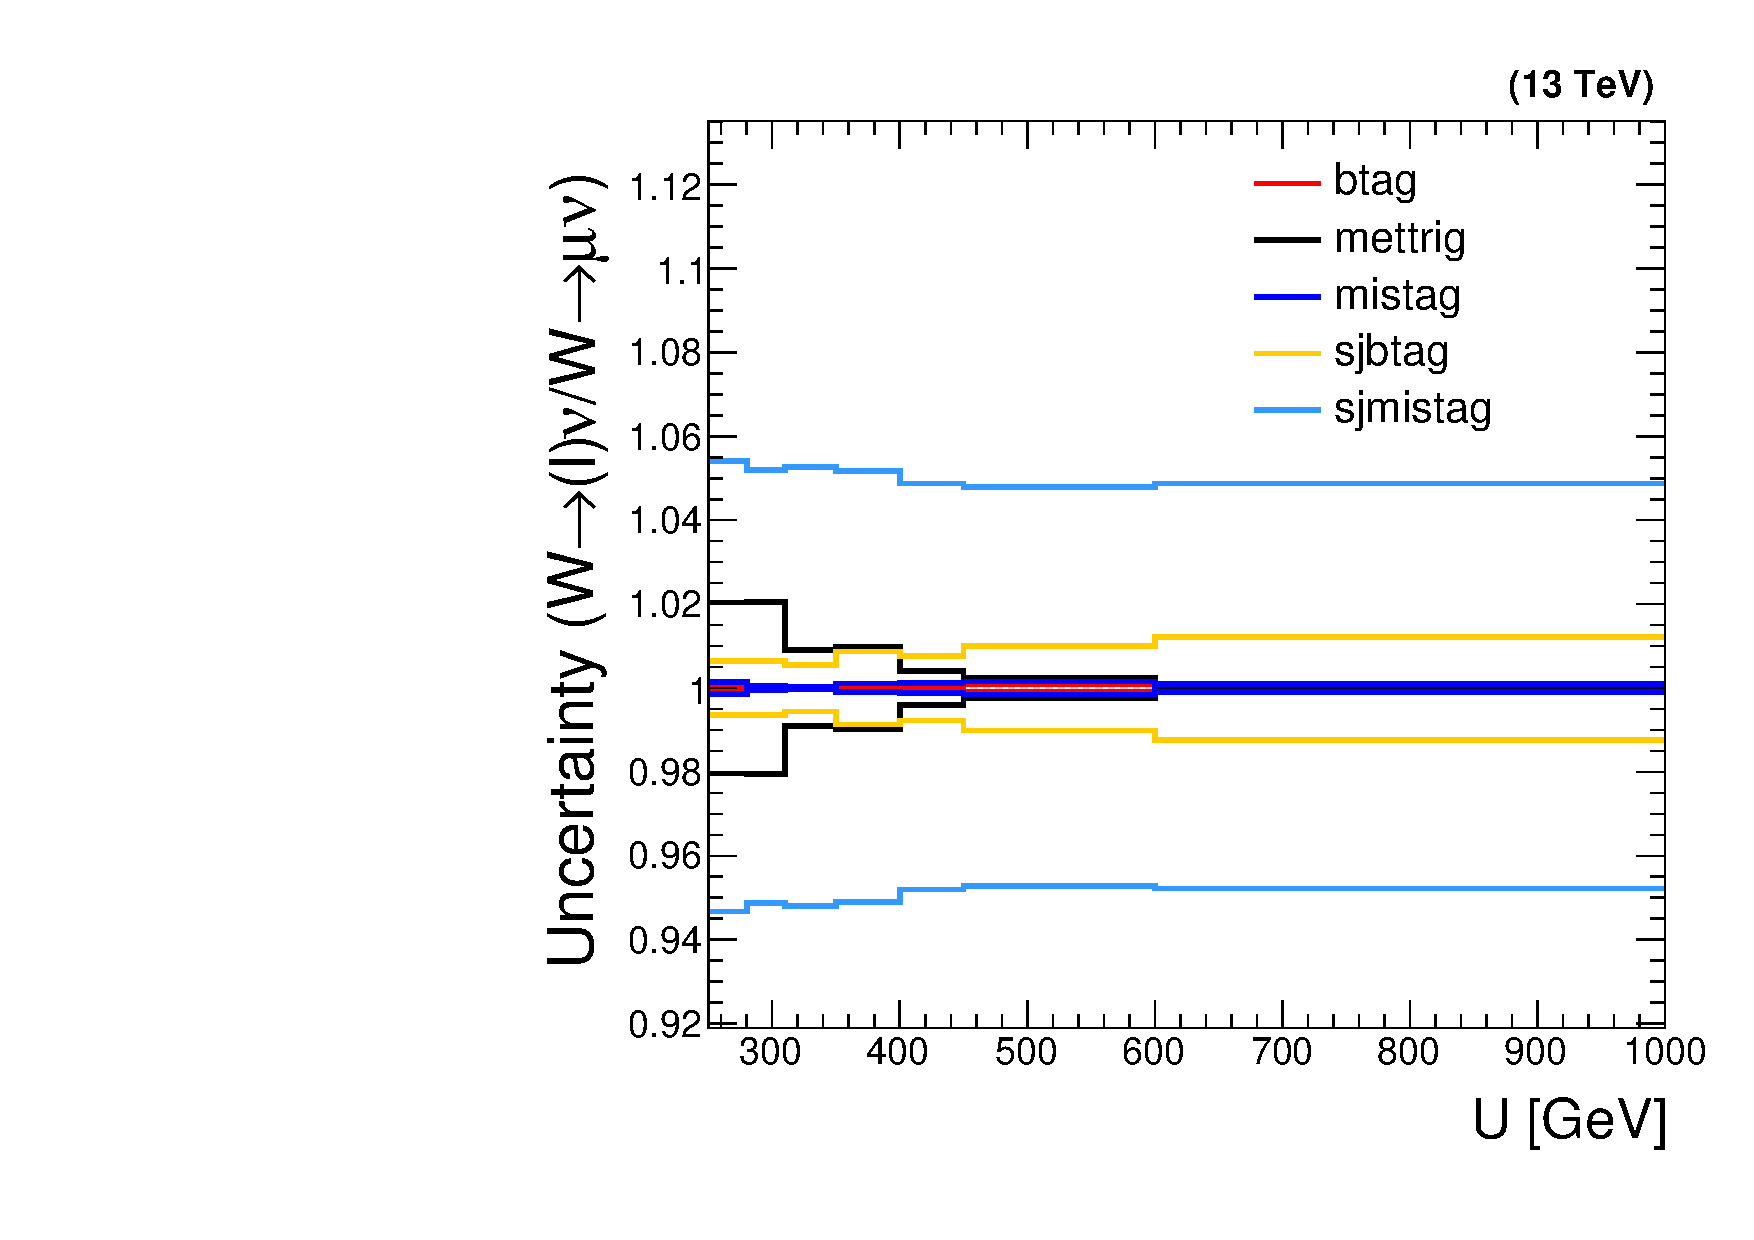
\includegraphics[width=0.49\textwidth]{figures/monotop/uncertainties/variations_singlemuonw.pdf}
            \caption{Tight $\T{\mu}{W}$}
        \end{subfigure}
        \begin{subfigure}[t]{0.49\textwidth}
            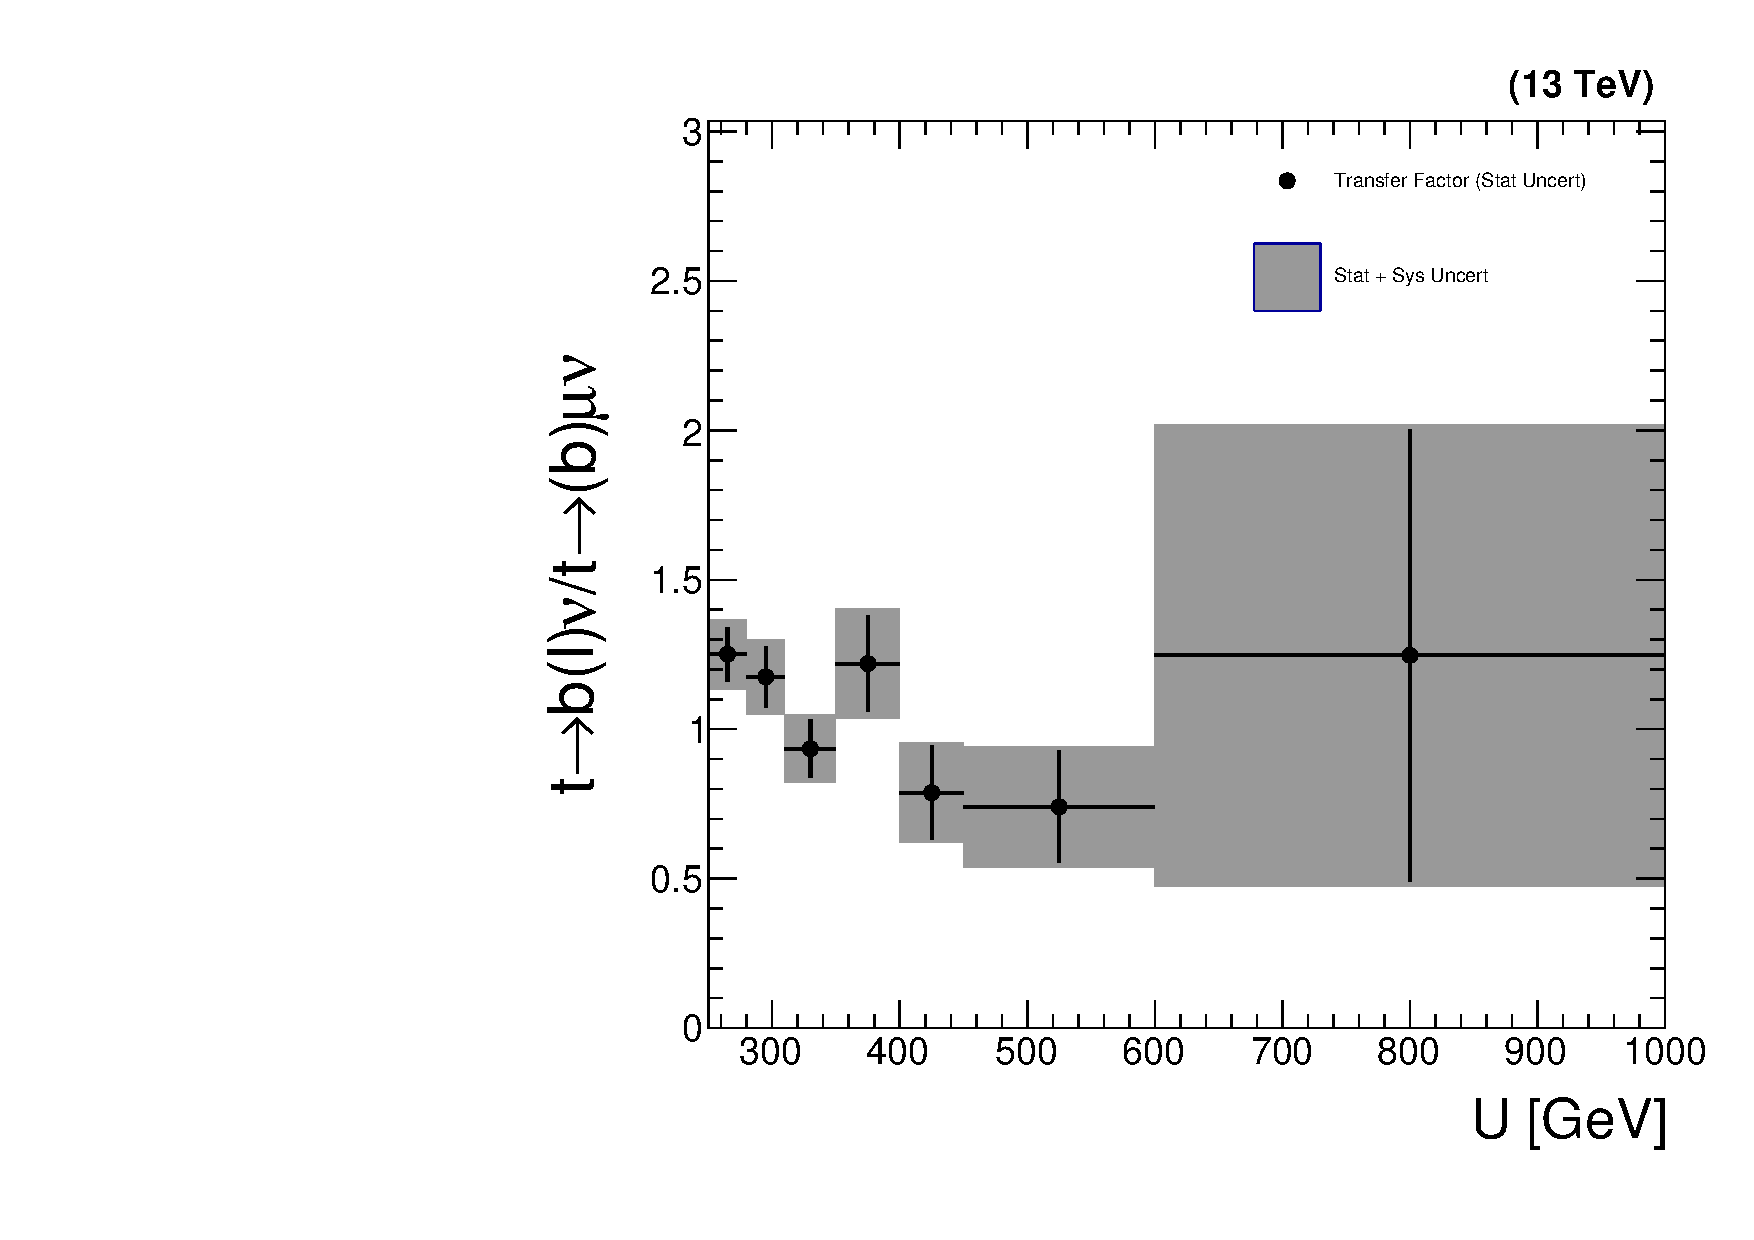
\includegraphics[width=0.49\textwidth]{figures/monotop/xfer/rfactor_singlemuonwtop_loose.pdf}
            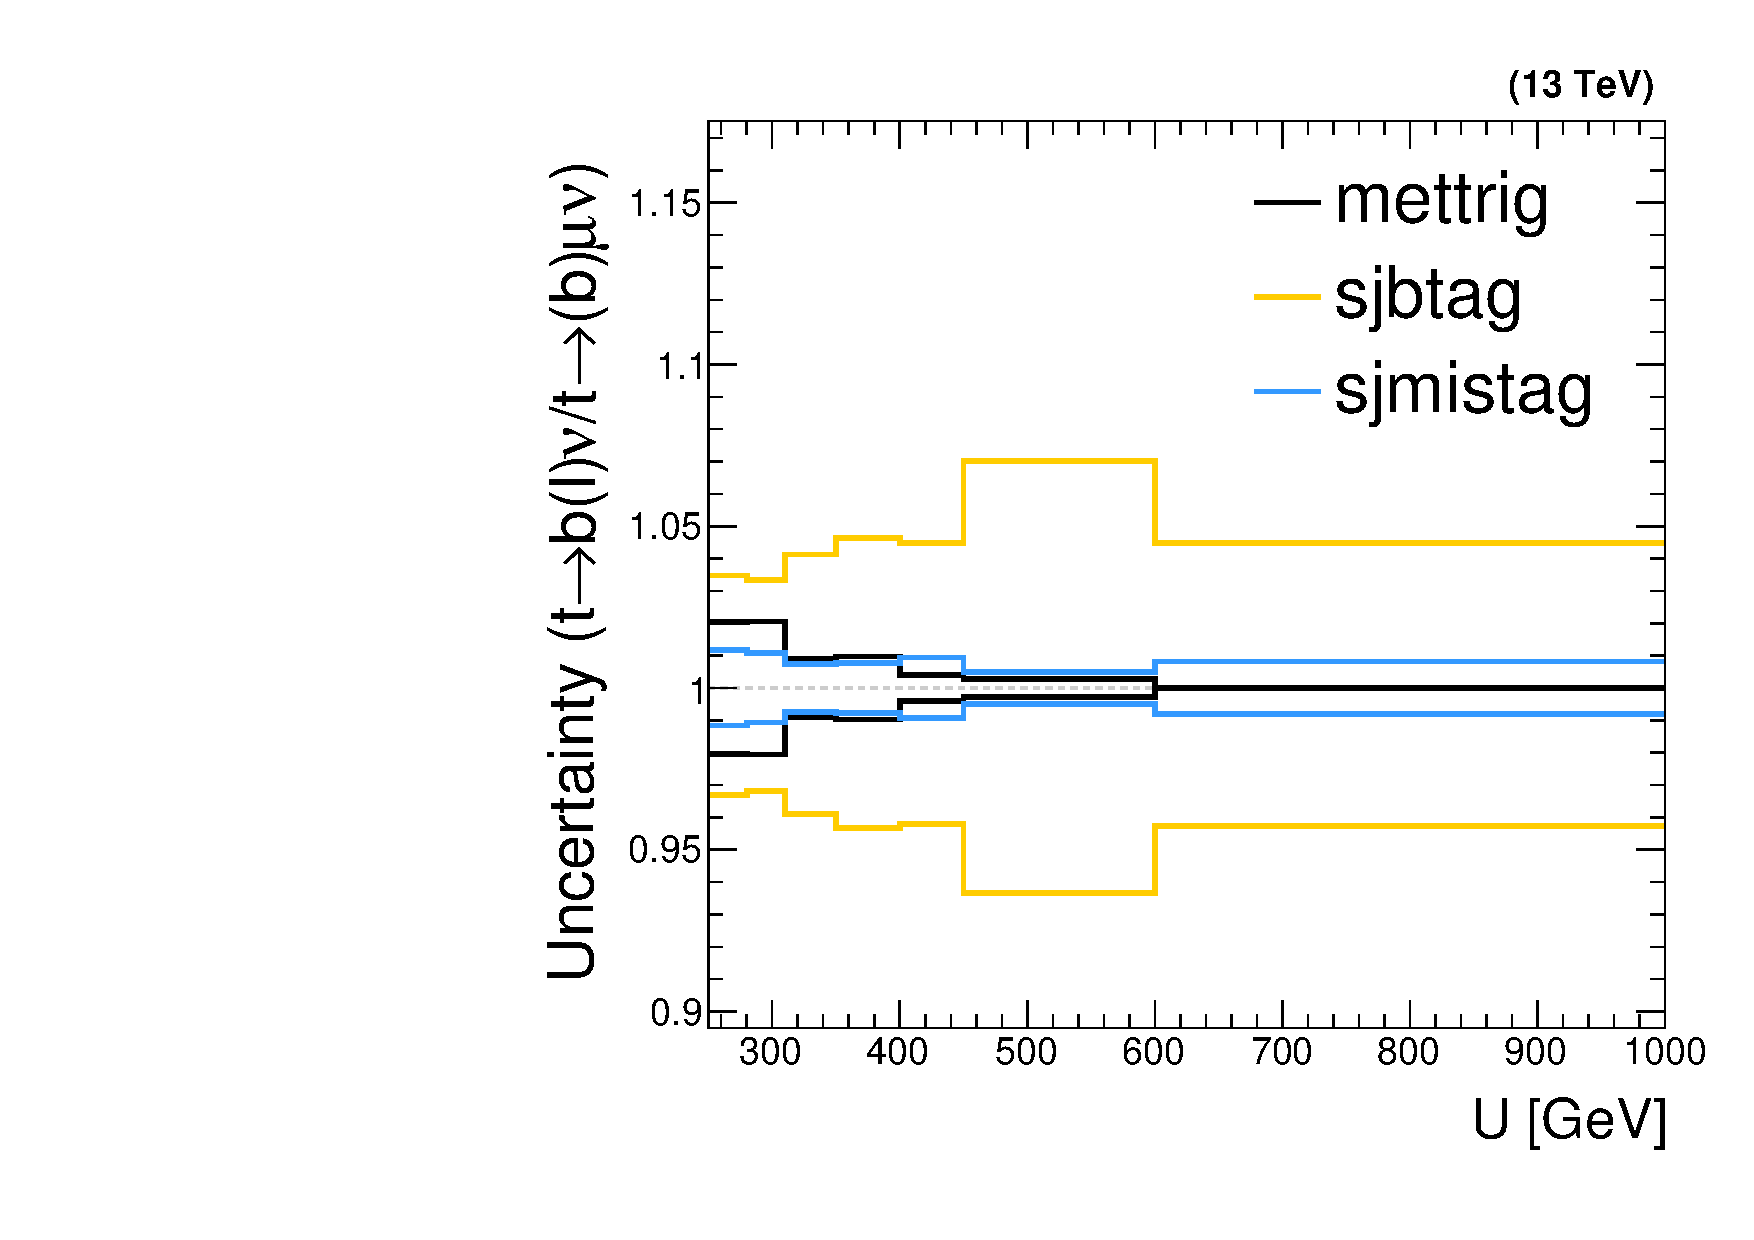
\includegraphics[width=0.49\textwidth]{figures/monotop/uncertainties/variations_singlemuonwtop_loose.pdf}
            \caption{Loose $\T{\mu}{\ttbar}$}
        \end{subfigure}
        \begin{subfigure}[t]{0.49\textwidth}
            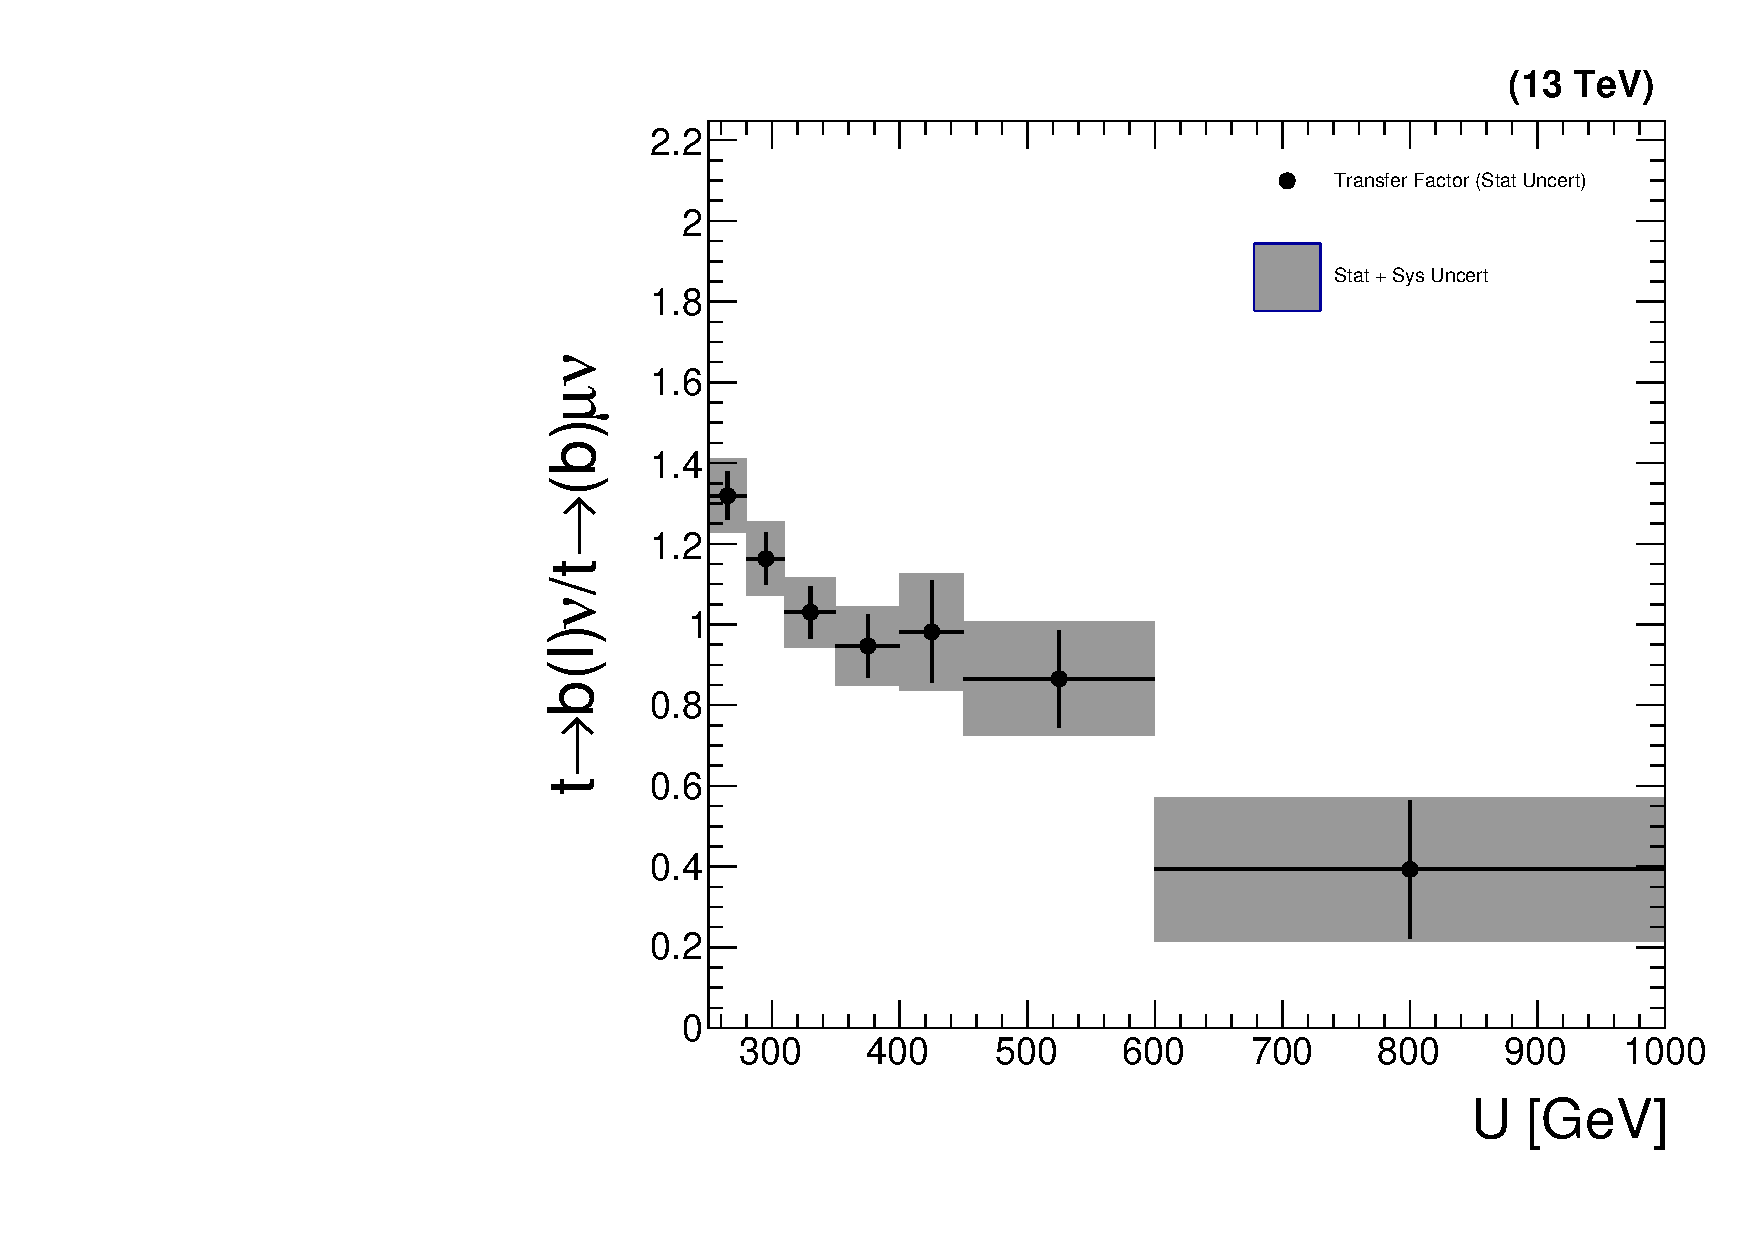
\includegraphics[width=0.49\textwidth]{figures/monotop/xfer/rfactor_singlemuonwtop.pdf}
            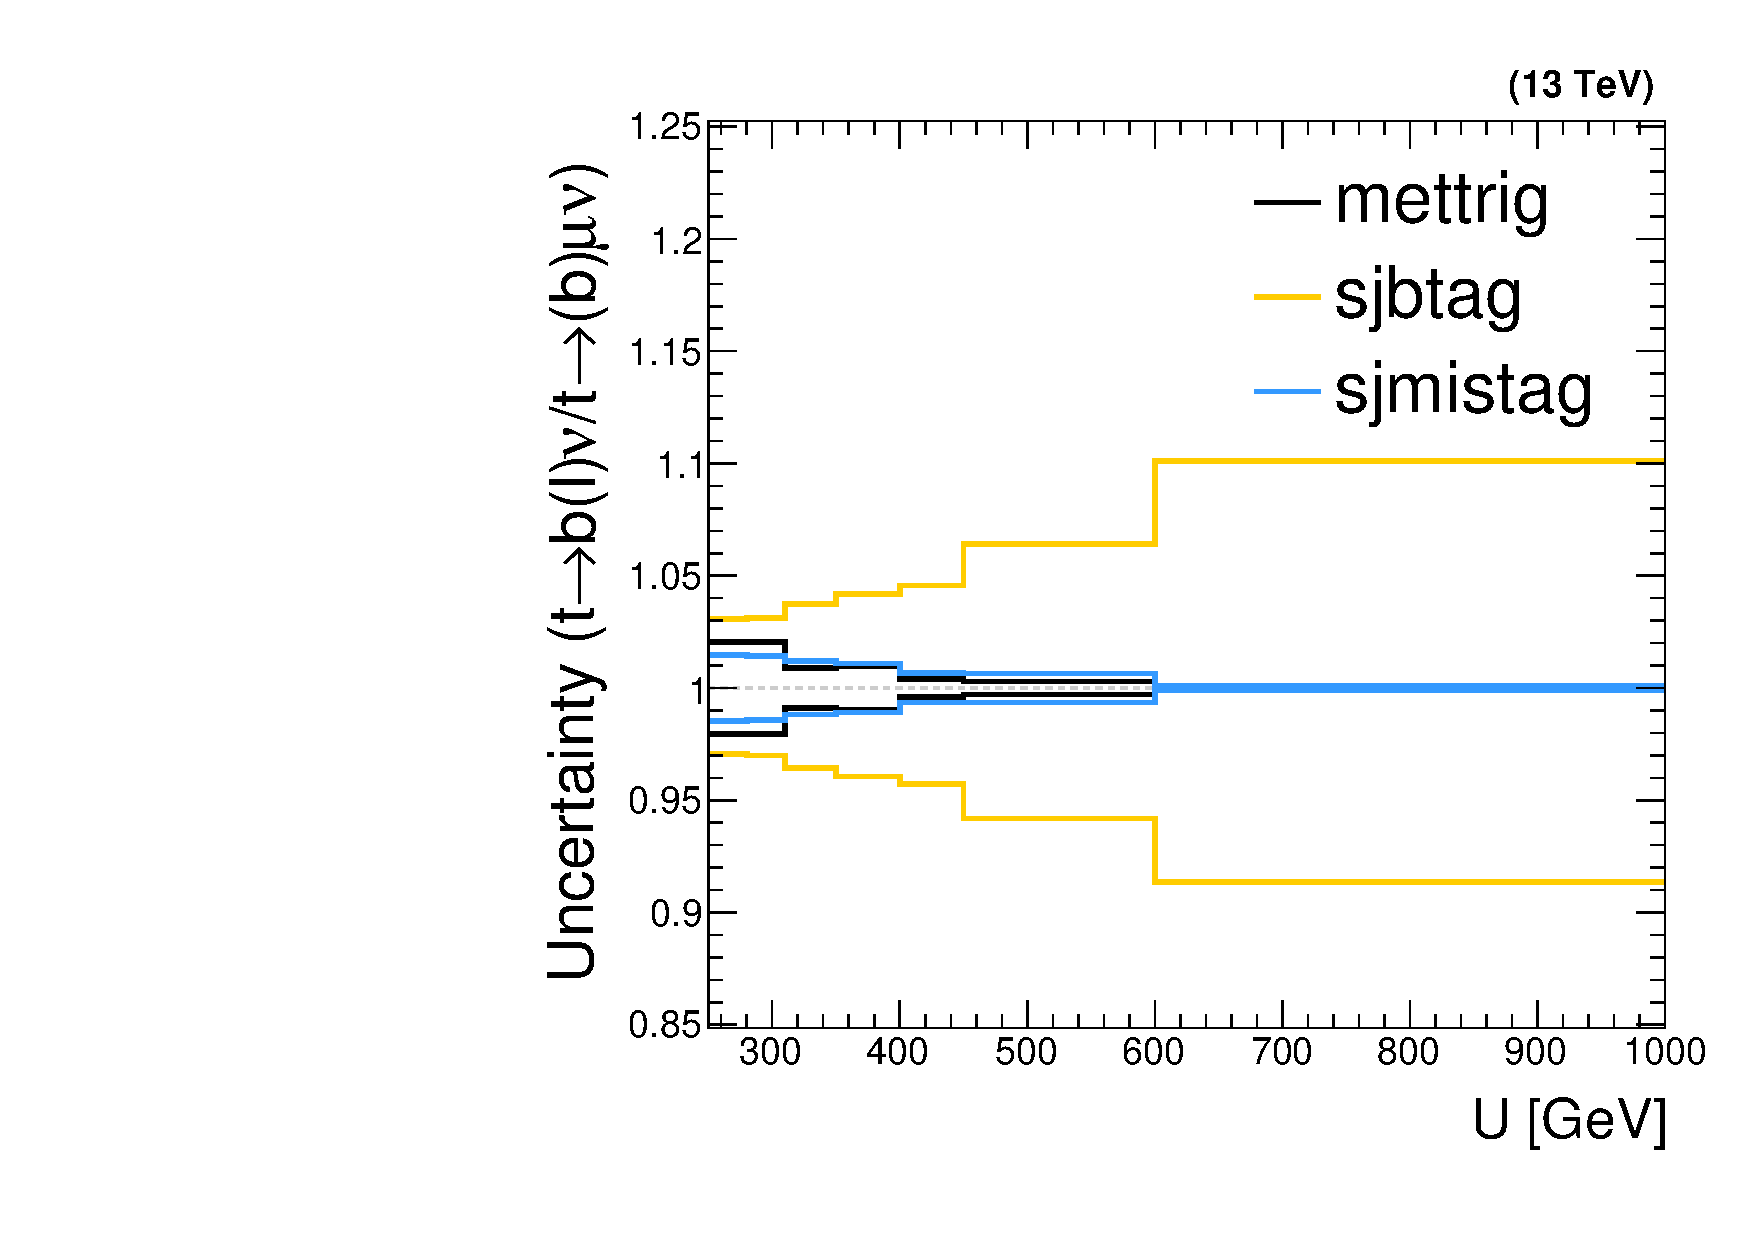
\includegraphics[width=0.49\textwidth]{figures/monotop/uncertainties/variations_singlemuonwtop.pdf}
            \caption{Tight $\T{\mu}{\ttbar}$}
        \end{subfigure}
        \caption{The transfer factors $\T{b\mu}{t\bar{t}}$, $\T{\mu}{W}$, and $\T{\mu}{t\bar{t}}$; and corresponding shape uncertainties.}
        \label{fig:mt:mn_xfer}
    \end{center}
\end{figure}

\begin{table}[]
    \begin{center}
    \caption{Uncertainties affecting the various single-muon extrapolations. 
            ``Shape'' uncertainties have different priors for each bin, but are assumed to be correlated across bins.}
    \label{tab:mt:zmm_uncs}
    \begin{tabular}{lcccl}
        Uncertainty                   & 1 s.d. ($\T{b\mu}{\ttbar}$) & 1 s.d. ($\T{\mu}{W}$) & 1 s.d. ($\T{\mu}{\ttbar}$)  & Notes \\ 
        \hline \hline 
        $\mu$ ID                      & 1\%                         & 1\%                   & 1\%                         & \\ 
        $\mu$ track                   & 0.5\%                       & 0.5\%                 & 0.5\%                       & \\ 
        $\tau_\mathrm{h}$ veto        & 3\%                         & 3\%                   &  3\%                        & \\ 
        $W$+heavy flavor              &                             & 3\%                   &                             & \\ 
        Trigger                       & 0-2\%                       & 0-2\%                 &  0-2\%                      & Shape \\ 
        $b$-tag                       & $2\%$                       & $\sim0.5\%$           &  3-6\%                      & Shape \\ 
        $udcsg$-mistag                & 1\%                         & 5\%                   & 1\%                         & Shape \\ 
    \end{tabular}
\end{center}
\end{table}

As we added the $ee$ CRs to complement the $\mu\mu$ CRs, we also add $be$ ($e$) CRs to augment the statistical power of the $b\mu$ ($\mu$) CRs, especially at high recoil.
Figures~\ref{fig:mt:prefit_en}~and~\ref{fig:mt:en_xfer} respectively show some kinematic distributions and the transfer factors corresponding to these electron constraints.

\begin{figure}[]
    \begin{center}
        \begin{subfigure}[t]{0.32\textwidth}
            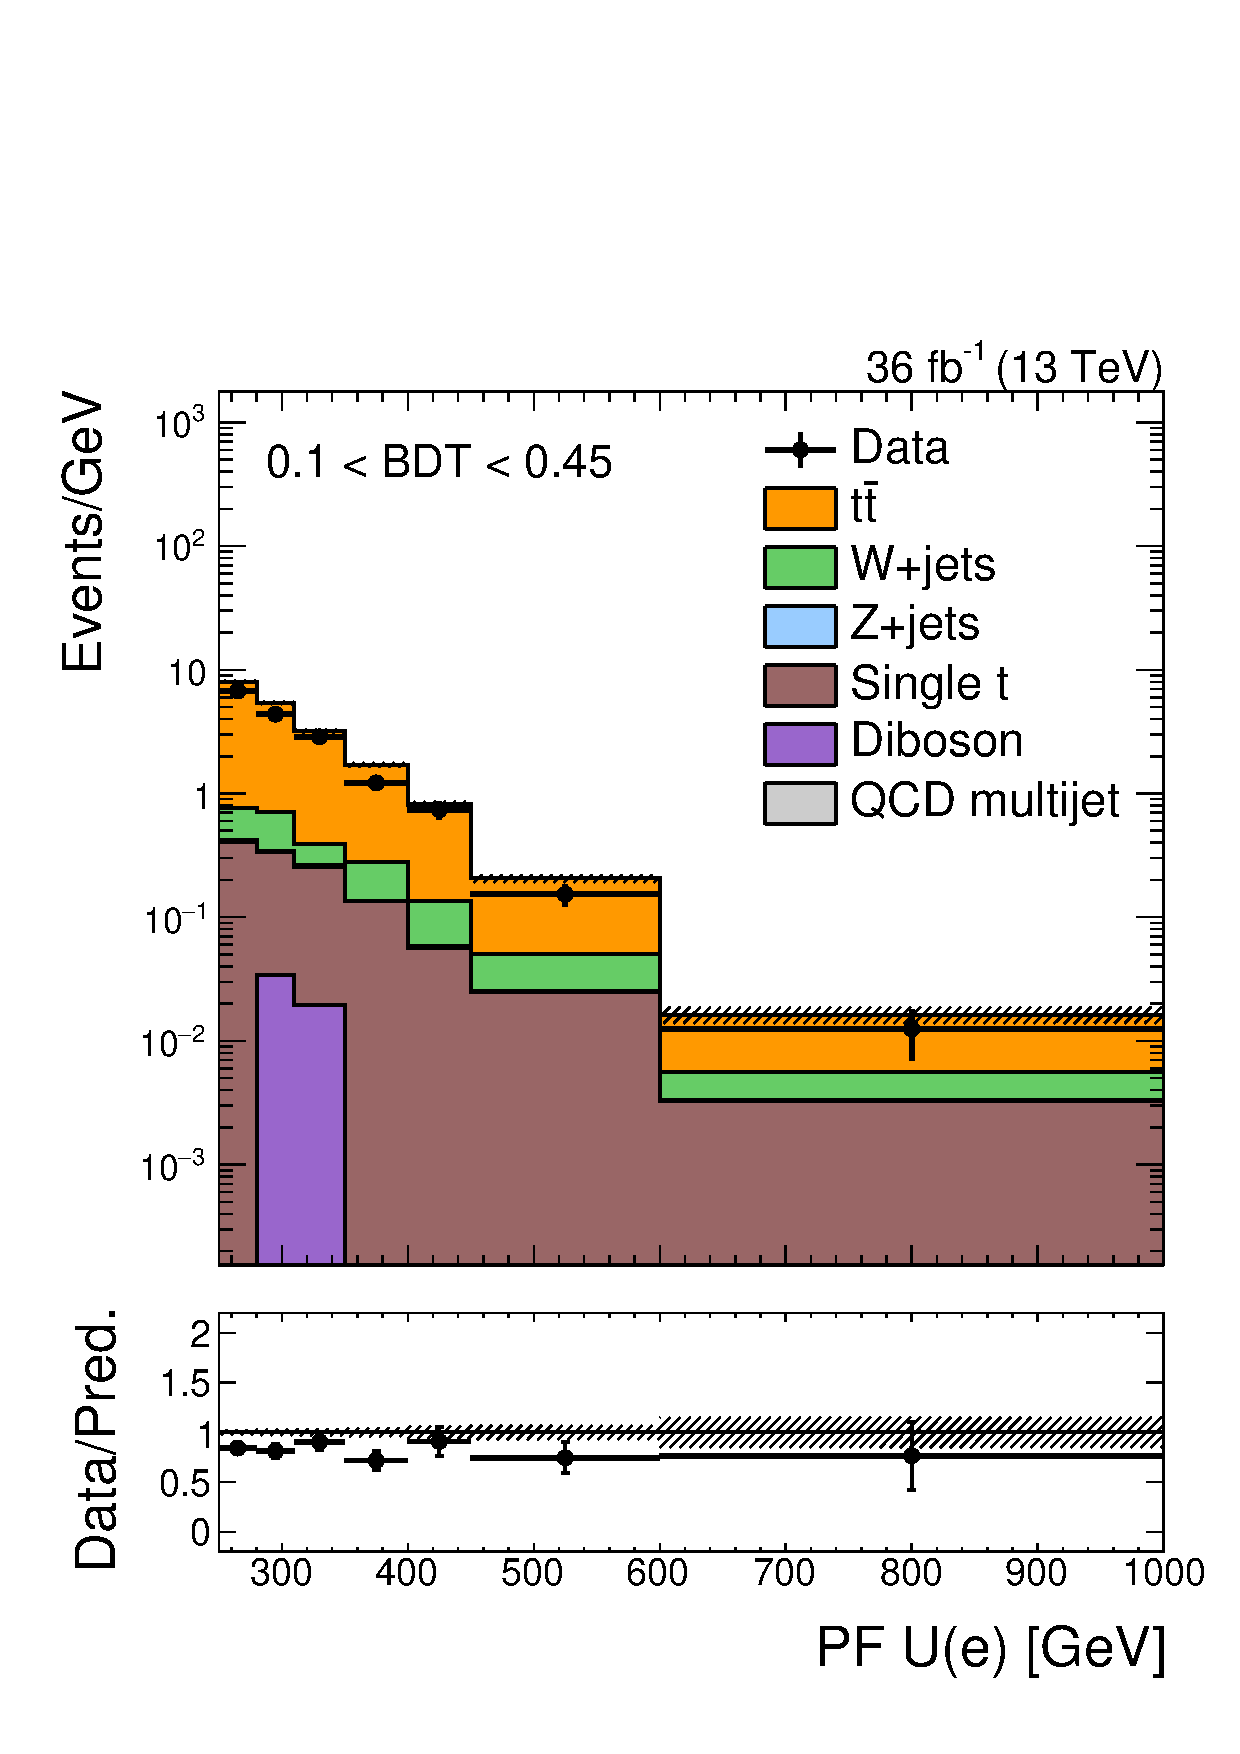
\includegraphics[width=\textwidth]{figures/monotop/prefit/singleelectrontop_loose_pfUWmag_logy.pdf}
            \caption{$U$ in loose $be$ CR}
        \end{subfigure}
        \begin{subfigure}[t]{0.32\textwidth}
            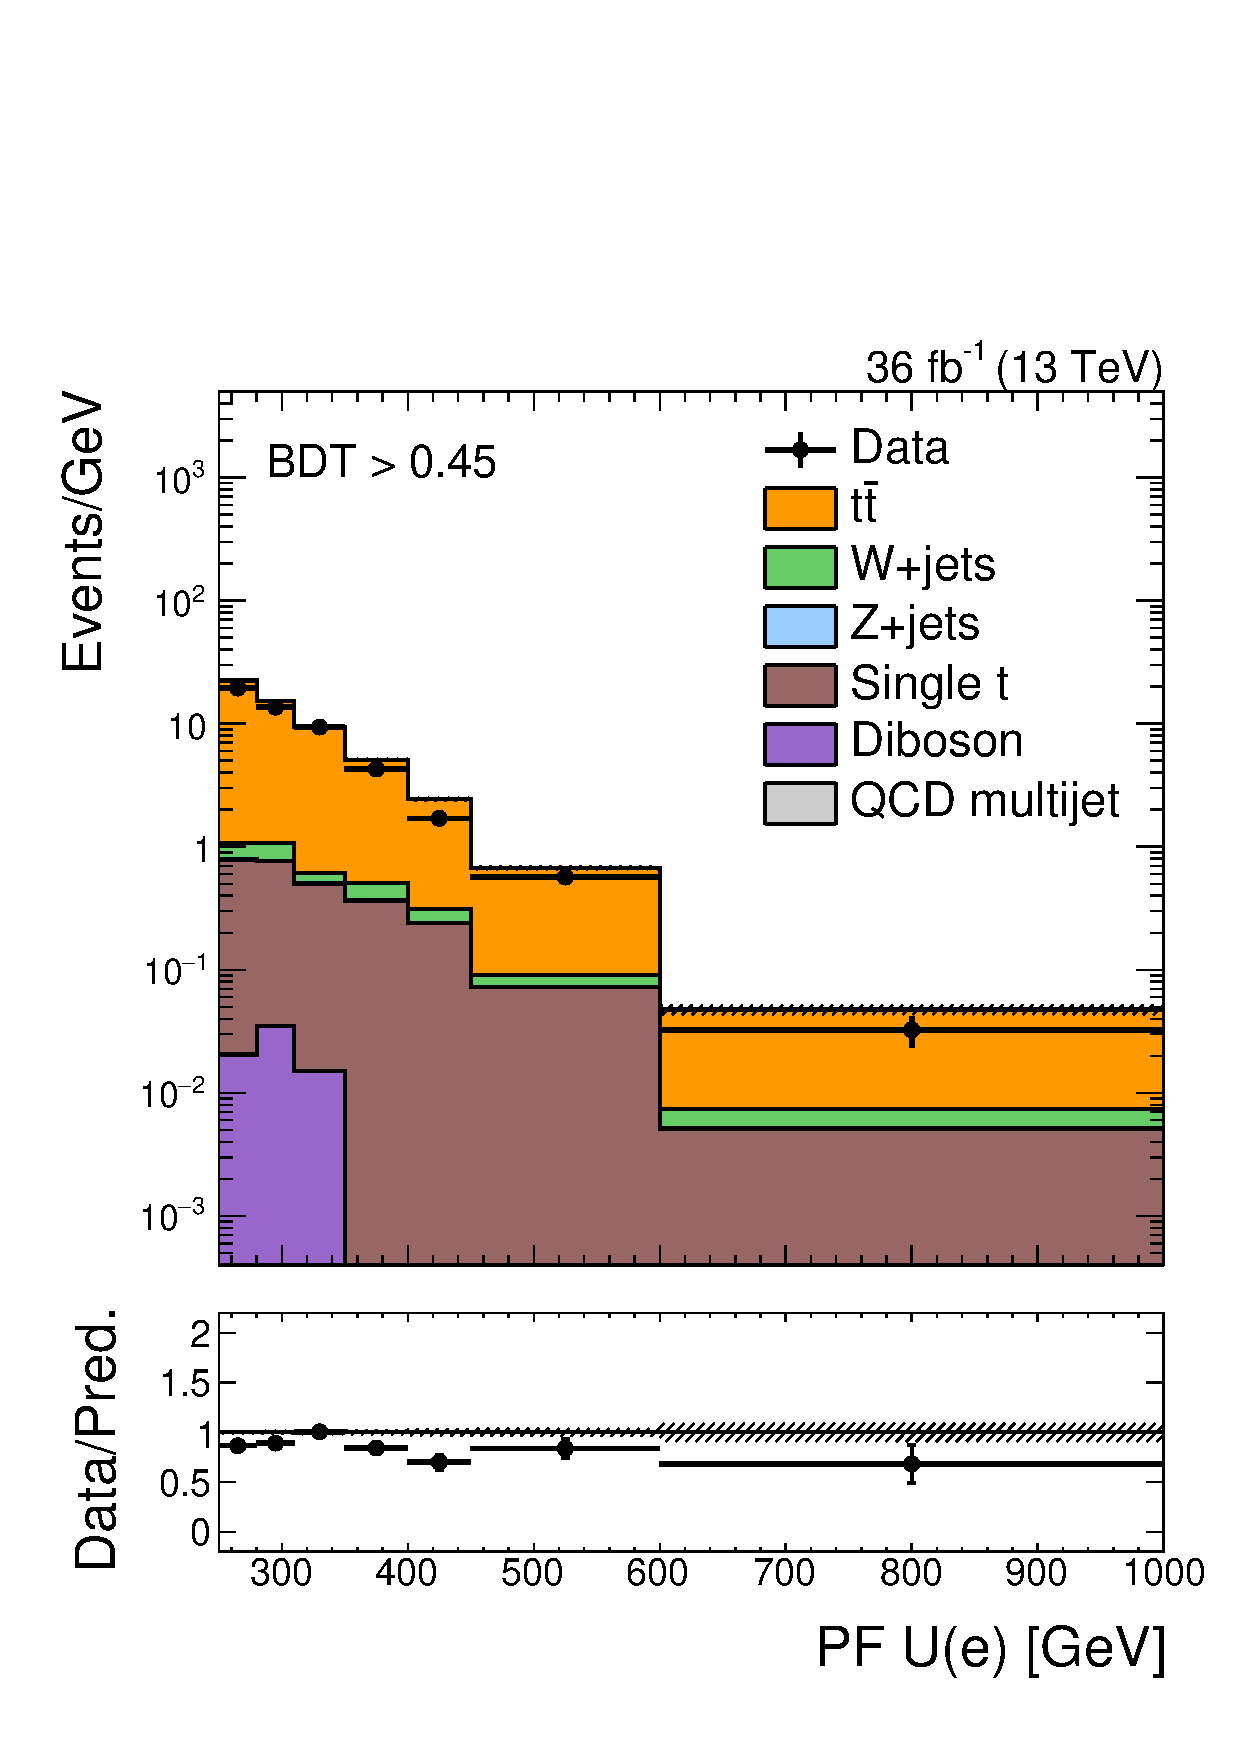
\includegraphics[width=\textwidth]{figures/monotop/prefit/singleelectrontop_tight_pfUWmag_logy.pdf}
            \caption{$U$ in tight $be$ CR}
        \end{subfigure}
        \begin{subfigure}[t]{0.32\textwidth}
            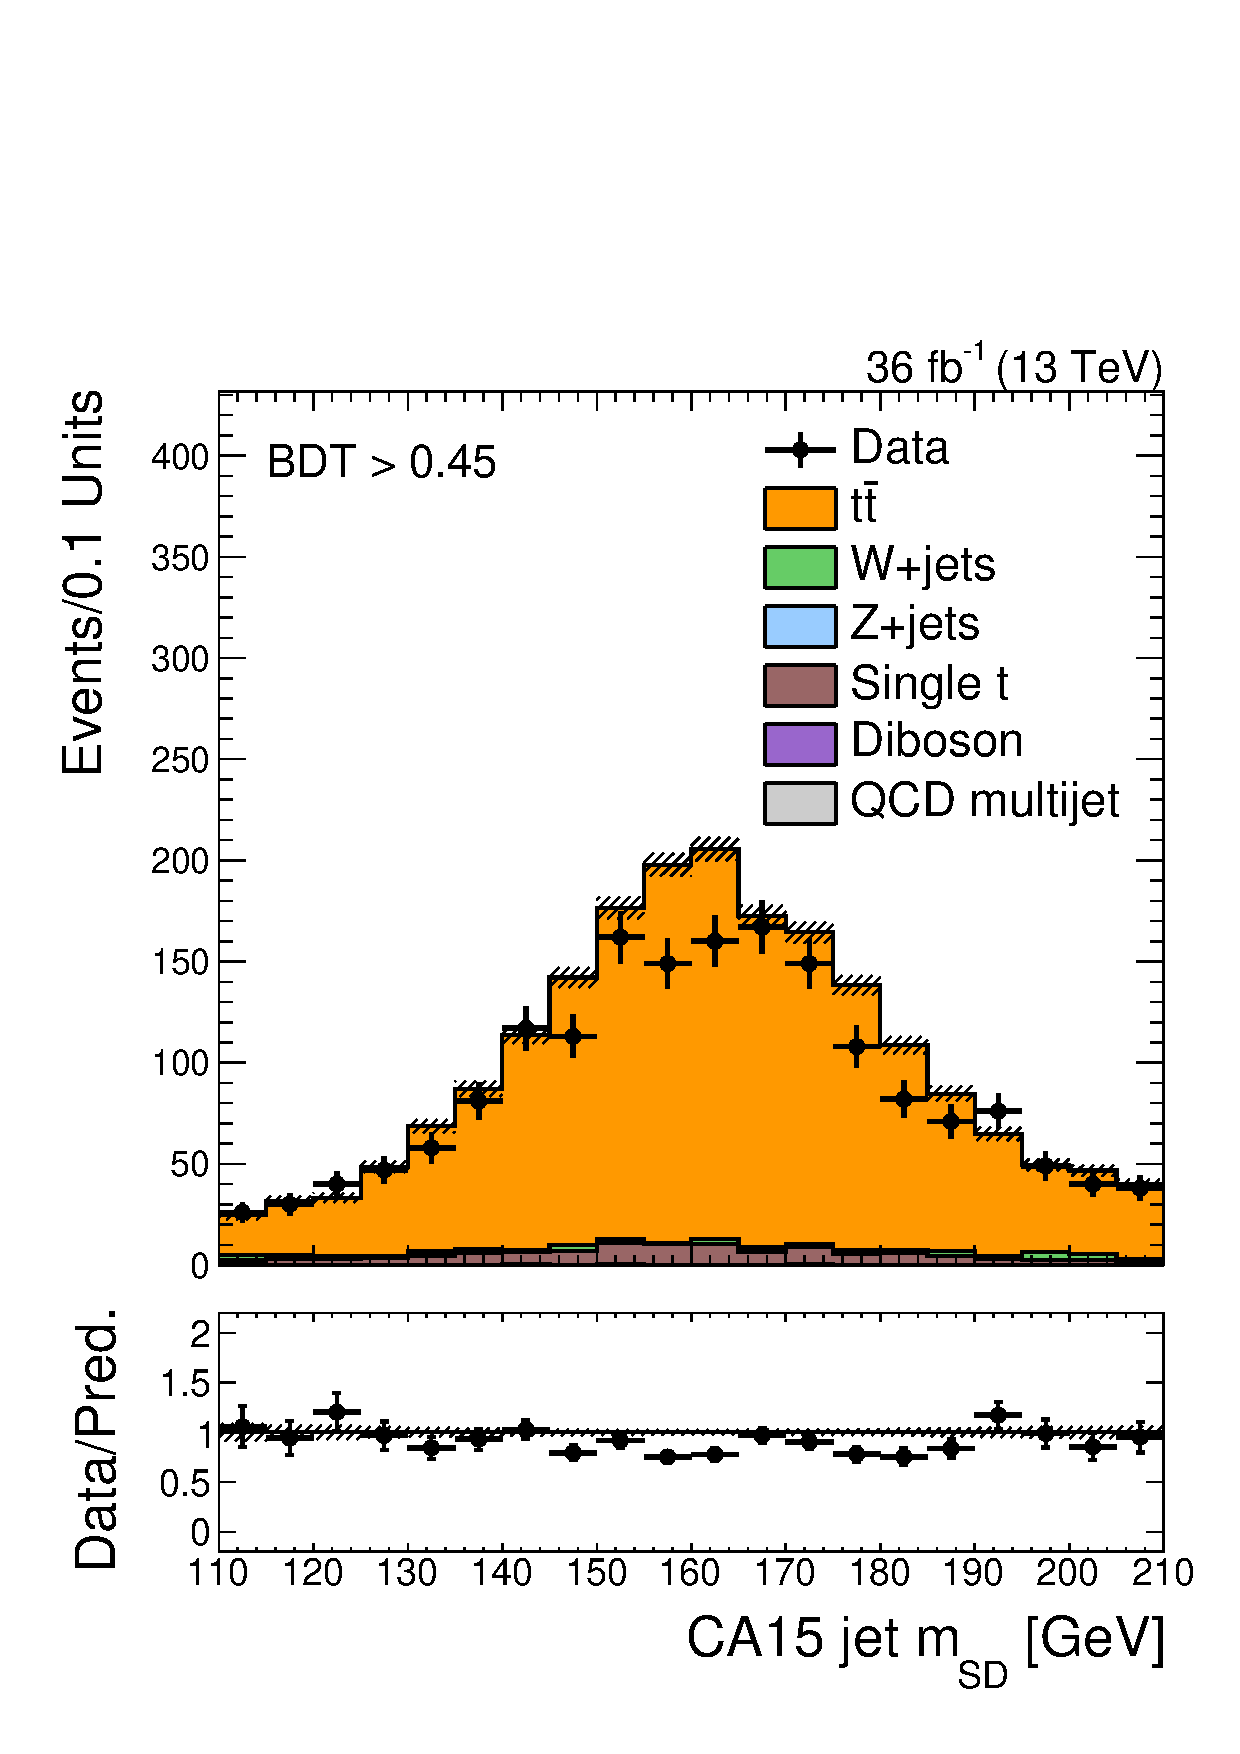
\includegraphics[width=\textwidth]{figures/monotop/prefit/singleelectrontop_tight_fj1MSD.pdf}
            \caption{$m_\mathrm{SD}$ in tight $be$ CR}
        \end{subfigure}
        \begin{subfigure}[t]{0.32\textwidth}
            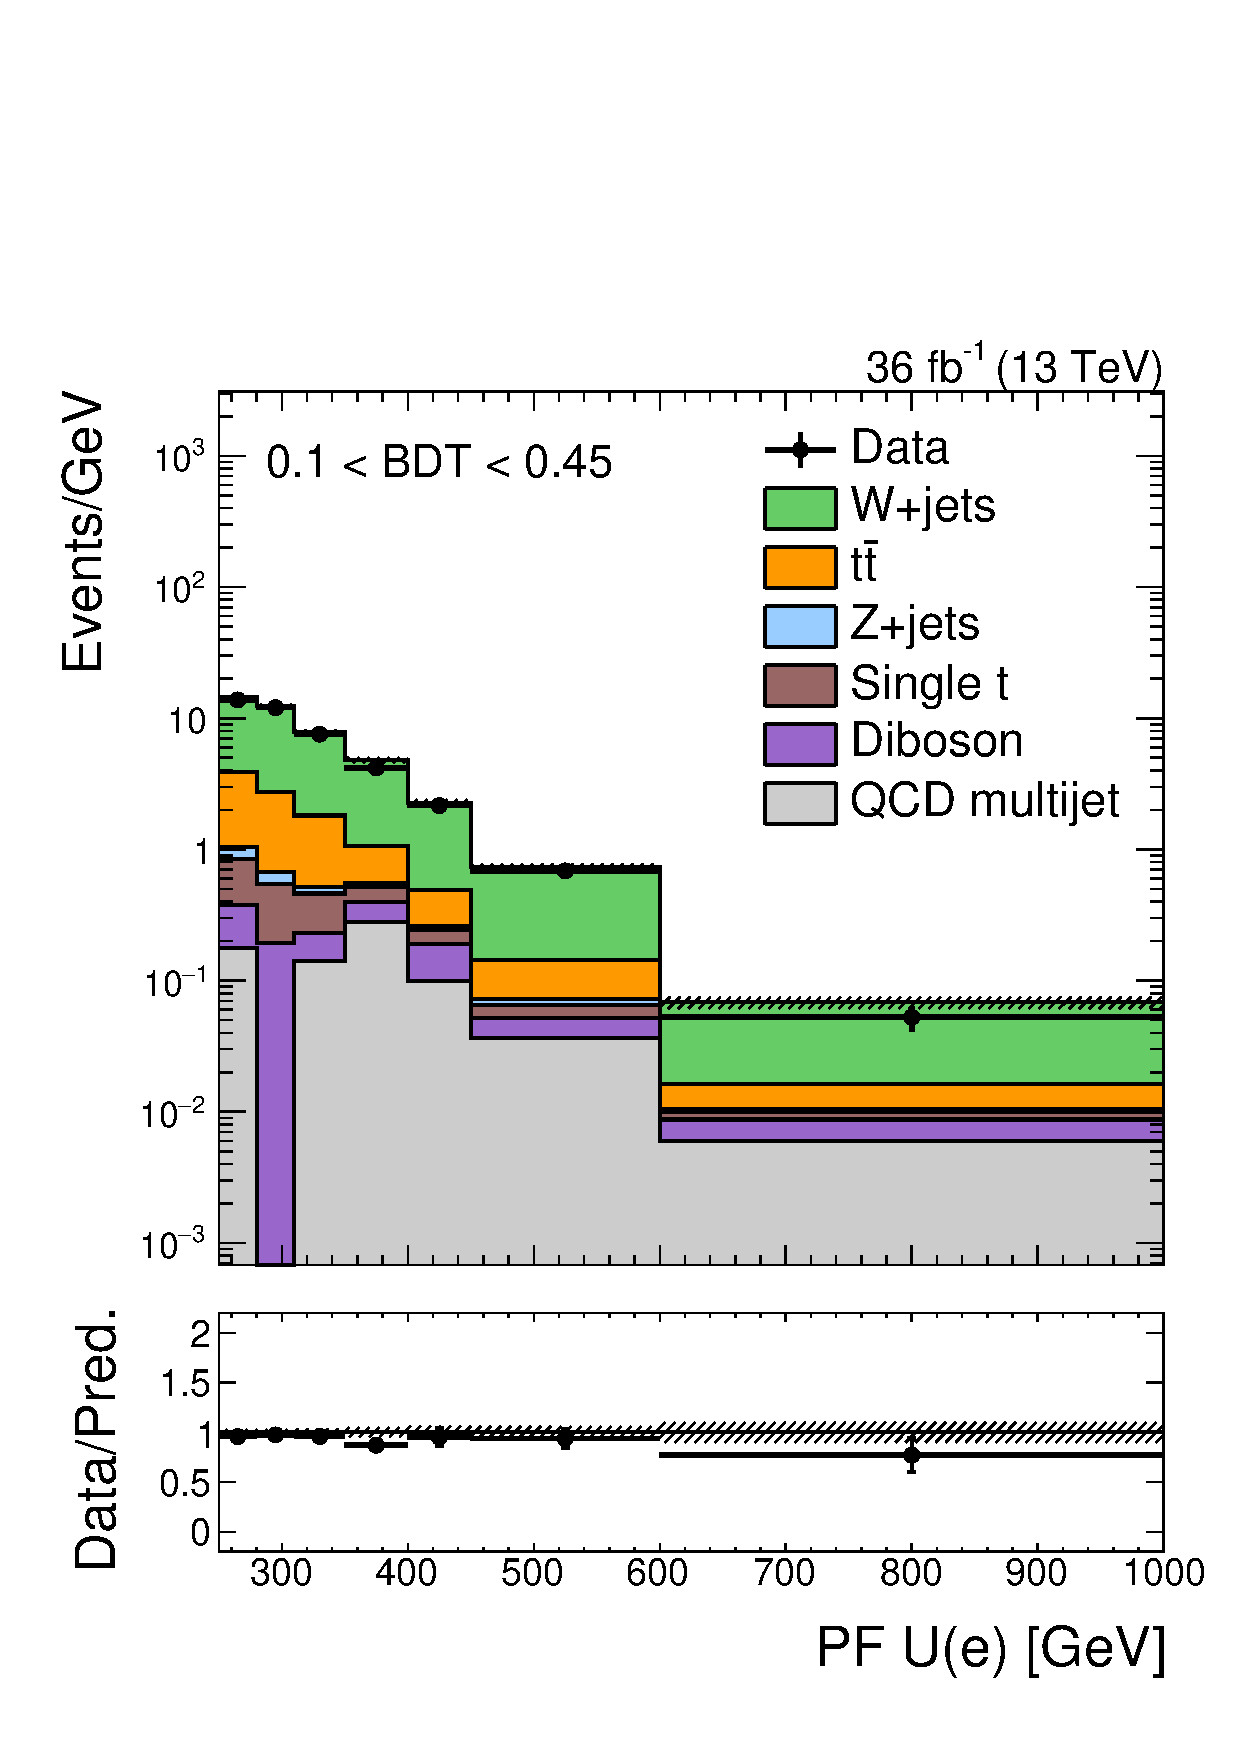
\includegraphics[width=\textwidth]{figures/monotop/prefit/singleelectronw_loose_pfUWmag_logy.pdf}
            \caption{$U$ in loose $e$ CR}
        \end{subfigure}
        \begin{subfigure}[t]{0.32\textwidth}
            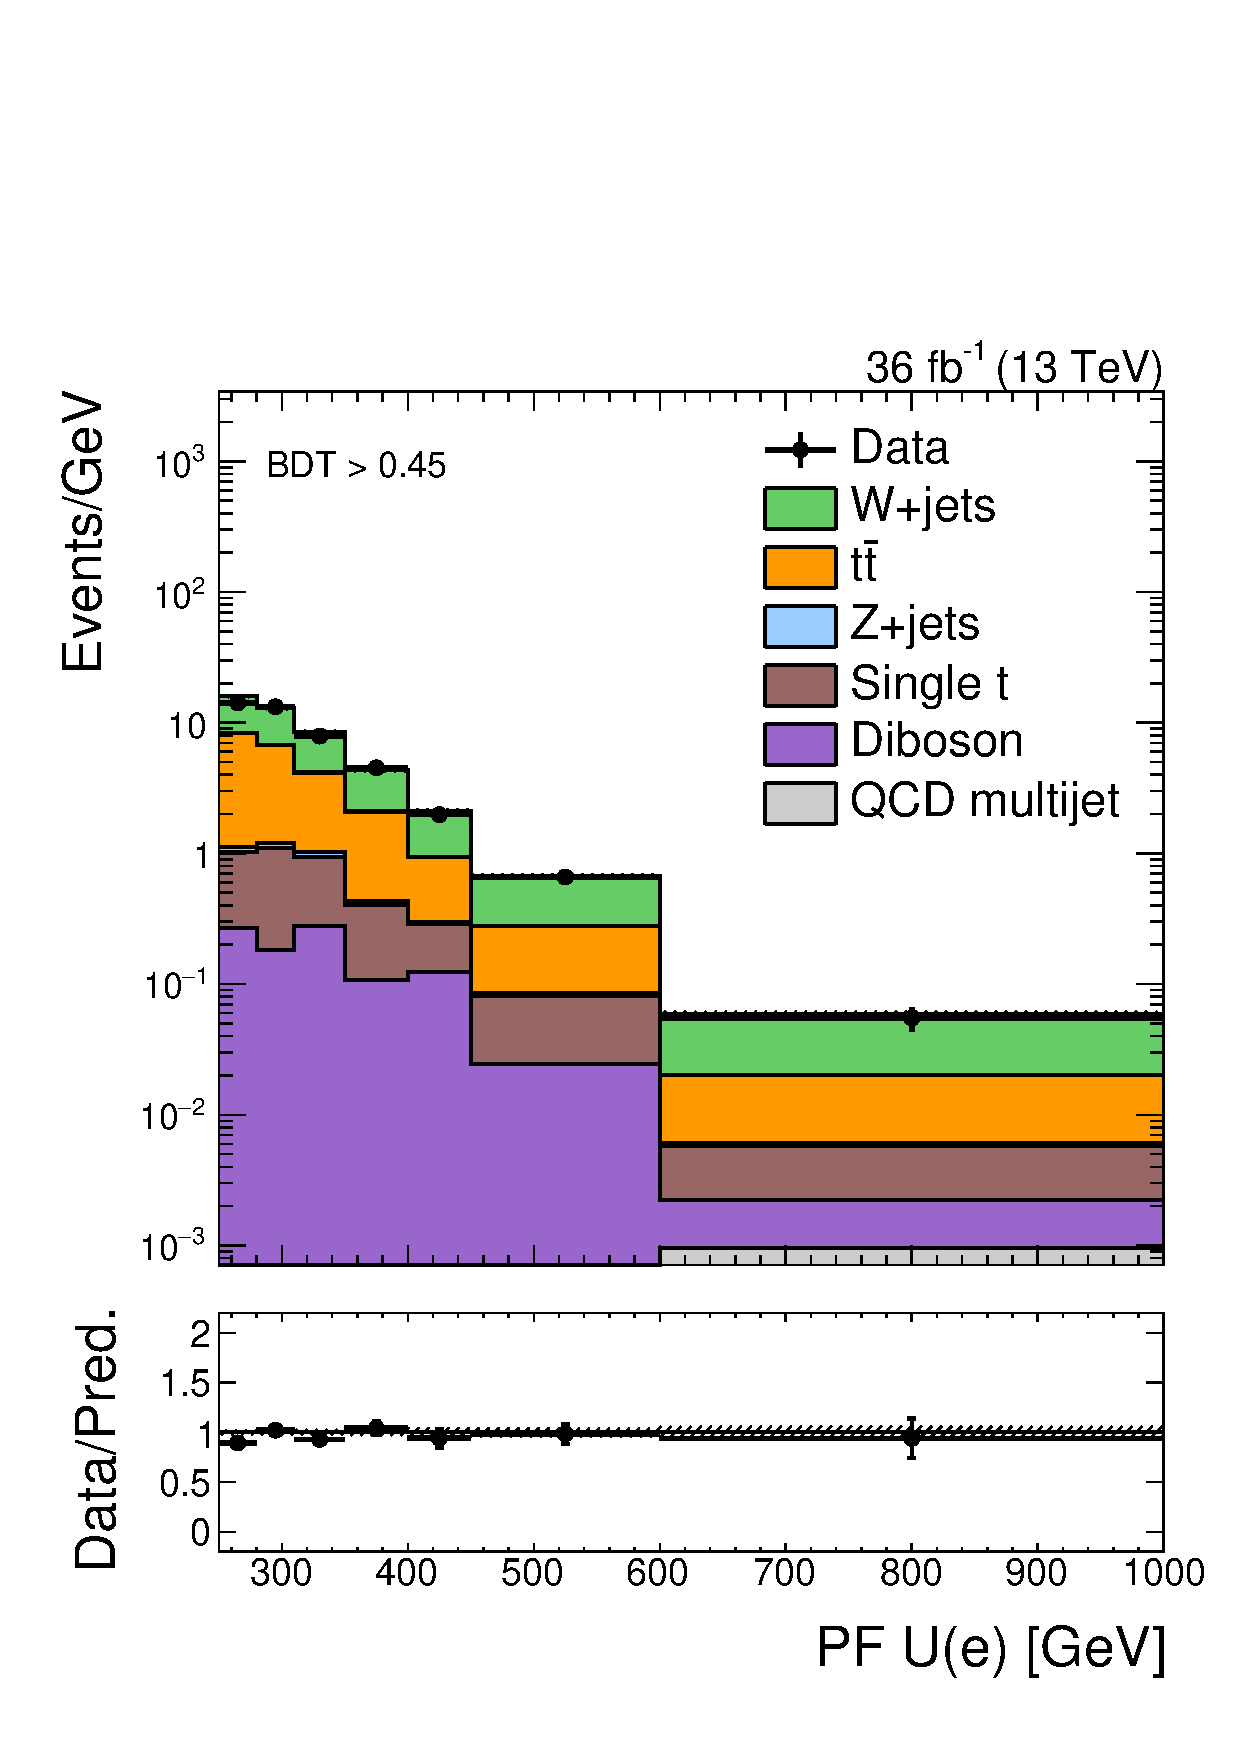
\includegraphics[width=\textwidth]{figures/monotop/prefit/singleelectronw_tight_pfUWmag_logy.pdf}
            \caption{$U$ in tight $e$ CR}
        \end{subfigure}
        \begin{subfigure}[t]{0.32\textwidth}
            \includegraphics[width=\textwidth]{figures/monotop/prefit/singleelectronw_tight_fj1MSD.pdf}
            \caption{$m_\mathrm{SD}$ in tight $e$ CR}
        \end{subfigure}
        \caption{Various kinematic distributions in the mono-top $be$ CRs (top) and $e$ CRs (bottom).}
        \label{fig:mt:prefit_en}
    \end{center}
\end{figure}

\begin{figure}[]
    \begin{center}
        \begin{subfigure}[t]{0.32\textwidth}
            \includegraphics[width=\textwidth]{figures/monotop/xfer/rfactor_singleelectrontop_loose.pdf}
            \caption{Loose $\T{be}{t\bar{t}}$}
        \end{subfigure}
        \begin{subfigure}[t]{0.32\textwidth}
            \includegraphics[width=\textwidth]{figures/monotop/xfer/rfactor_singleelectronw_loose.pdf}
            \caption{Loose $\T{e}{W}$}
        \end{subfigure}
        \begin{subfigure}[t]{0.32\textwidth}
            \includegraphics[width=\textwidth]{figures/monotop/xfer/rfactor_singleelectronwtop_loose.pdf}
            \caption{Loose $\T{e}{\ttbar}$}
        \end{subfigure}
        \begin{subfigure}[t]{0.32\textwidth}
            \includegraphics[width=\textwidth]{figures/monotop/xfer/rfactor_singleelectrontop.pdf}
            \caption{Tight $\T{be}{t\bar{t}}$}
        \end{subfigure}
        \begin{subfigure}[t]{0.32\textwidth}
            \includegraphics[width=\textwidth]{figures/monotop/xfer/rfactor_singleelectronw.pdf}
            \caption{Tight $\T{e}{W}$}
        \end{subfigure}
        \begin{subfigure}[t]{0.32\textwidth}
            \includegraphics[width=\textwidth]{figures/monotop/xfer/rfactor_singleelectronwtop.pdf}
            \caption{Tight $\T{e}{\ttbar}$}
        \end{subfigure}
        \caption{The transfer factors $\T{be}{t\bar{t}}$, $\T{e}{W}$, and $\T{e}{t\bar{t}}$}
        \label{fig:mt:en_xfer}
    \end{center}
\end{figure}

Having defined (almost all of) the CRs and transfer factors, we can write down a complete likelihood for the mono-top search:
\begin{align}
    \mathcal{L}\left(\bm{d}~|~ \mu,\muz,\muw,\mut,\bm{\theta}\right) = \hspace{-40mm} & \nonumber \\
    \prod_{i\in\mathrm{bins}} & \left[ 
    \pois\left(d^{\mathrm{SR}}_{i} ~\Big|~ \mu S^{\mathrm{SR}}_{i}(\bm\theta)  + \muzi + \muwi + \muti + B^{\mathrm{SR}}_{i}(\bm\theta)\right) \vphantom{\frac{\muzi}{\Ti{\mu\mu}{Z}(\bm\theta)}}\right. \nonumber \\
    & \phantom{\Big[} \times \prod_{X=\mu\mu,ee} \pois\left(d^{X}_i~\Big|~ \frac{\muzi}{\Ti{X}{Z}(\bm\theta)} + B^{X}_i(\bm\theta) \right) \nonumber \\  
    & \phantom{\Big[} \times \prod_{X=b\mu,be}\pois\left(d^{X}_i~\Big|~ \frac{\muti}{\Ti{X}{\ttbar}(\bm\theta)} + B^{X}_i(\bm\theta) \right) \nonumber \\ 
    & \phantom{\Big[} \times \prod_{X=\mu,e} \pois\left(\left.d^{X}_i~\Big|~ \frac{\muwi}{\Ti{X}{W}(\bm\theta)} + \frac{\muti}{\Ti{X}{\ttbar}(\bm\theta)} + B^{X}_i(\bm\theta) \right) \right]  \times  \prod_{j=0}^{n_\theta} p_j(\theta_j)
\end{align}

\subsection{Theoretically-limited extrapolations}
\label{sec:mt:smtheory}

Despite the combination of the $\mu\mu$ and $ee$ regions, there are still large statistical uncertainties in the estimate of $Z\rightarrow\nu\nu$ at high $U$.
This is apparent in Figure~\ref{fig:mt:prefit_dielectron}, in which exactly one event is observed in the last bin of the tight CR. 
The dilepton CRs are limited by $\sigma(pp\rightarrow Z\rightarrow\nu\nu) > \sigma(pp\rightarrow Z\rightarrow\ell^+\ell^-)$; accordingly, to alleviate this limitation, we look to a process with a much bigger cross-section.
In similar regions of final-state phase space, $\sigma(pp\rightarrow\gamma+\mathrm{jets}) \sim 30 \times \sigma(pp\rightarrow Z(\rightarrow\nu\nu)+\mathrm{jets})$. 
Therefore, it is natural to use the $\gamma$+jet production spectrum as a way to estimate the $Z$+jet spectrum.
As before, let us define another transfer factor:
\begin{equation}
    \Ti{\gamma}{\gamma} = \frac{N^\mathrm{SR}_i(Z\rightarrow\nu\nu)}{N_i^\gamma(\gamma)}
\end{equation}
However, unlike the $\T{X}{Y}$ we have discussed so far (which correlate similar processes, e.g. $Z\rightarrow\nu\nu/Z\rightarrow\mu\mu$), $\T{\gamma}{\gamma}$ is highly sensitive to the theoretical predictions of the $Z$ and $\gamma$ spectra.

To reduce the impact of higher-order effects on $\T\gamma\gamma$, we ensure that the numerator and denominator are predicted to as high an order as possible.
Leading-order MC is used to simulate $V$+jet processes, because higher-order simulations are much more computationally intensive.
We therefore choose to produce a less accurate LO simulation, as opposed to a more accurate, but statistically-limited, NLO simulation.
While producing sufficient NLO simulation for the analysis is prohibitive, we can compute certain inclusive distributions at NLO.
Since $U\approx \pt^V$ is the quantity of interest in this analysis, we want to ensure this distribution is accurately predicted.
It is clear from Figure~\ref{fig:mt:zlonlo} that adding an additional QCD order induces large corrections, both at low and high $\pt^V$.
In the LO simulation, we can obtain an estimate of the uncertainty due to NLO effects by varying the renormalization and factorization scales ($\mu_R,\mu_F$) by factors of two.
This is represented by the red envelope and grey band in Figure~\ref{fig:mt:zlonlo} and clearly is insufficient to cover NLO effects. 
Therefore, we compute a simple correction for the NLO QCD effects, known as a $k$-factor:
\begin{equation}
    k_{Z,\mathrm{QCD}}(\pt^Z) = \frac{d\sigma_\text{NLO QCD}(Z) / d\pt^Z}{d\sigma_\mathrm{LO}(Z) / d\pt^Z}
\end{equation}
We include another$k$-factor, $k_\mathrm{EWK}$, to correct for higher-order EWK effects.
Unlike $k_\mathrm{QCD}$, $k_\mathrm{EWK}$ is derived using a theoretical calculation~\cite{ewk2,ewk3,ewk1} instead of NLO simulation.
$k_\mathrm{EWK}$ covers NLO EWK terms, as well as large Sudakov logarithms that appear at high $\pt^V$ in the NNLO expansion (NLL). 

\begin{figure}[]
    \begin{center}
        \begin{subfigure}[t]{0.49\textwidth}
            \includegraphics[width=\textwidth]{figures/monotop/kfactors/zpt_logy.pdf}
            \caption{LO vs. NLO (QCD)}
        \end{subfigure}
        \begin{subfigure}[t]{0.49\textwidth}
            \includegraphics[width=\textwidth]{figures/monotop/kfactors/zcorr_ptv.pdf}
            \caption{$k$-factors}
        \end{subfigure}
        \caption{Theoretical predictions for $\pt^Z$ in $Z$+jet events and the corresponding $k$-factors. 
                 No detector simulation is applied in these figures; all quantities are directly from MC simulation of the physics process.
                 ``LO QCD uncertainty`` refers to an estimate of the effect of the QCD renormalization and factorization scales on the LO simulation.
                 The grey band in the ratio is the quadrature sum of the QCD and statistical uncertainties.}
        \label{fig:mt:zlonlo}
    \end{center}
\end{figure}

Figure~\ref{fig:mt:vlonlo} compares the $k$-factors for all three $V$+jet processes.
While there are similar trends as a function of $\pt^V$, it is clear that the corrections are quite different for each process.
Therefore, transfer factors like $\T\gamma\gamma$ are strongly sensitive to NLO effects, i.e.:
\begin{equation}
    \Ti{\gamma}{\gamma} = \frac{N^\mathrm{SR}_i(Z\rightarrow\nu\nu)}{N_i^\gamma(\gamma)} \neq \frac{N^\mathrm{SR,LO}_i(Z\rightarrow\nu\nu)}{N_i^{\gamma,\mathrm{LO}}(\gamma)}
\end{equation}

\begin{figure}[]
    \begin{center}
        \begin{subfigure}[t]{0.32\textwidth}
            \includegraphics[width=\textwidth]{figures/monotop/kfactors/zcorr_ptv.pdf}
            \caption{$Z$}
        \end{subfigure}
        \begin{subfigure}[t]{0.32\textwidth}
            \includegraphics[width=\textwidth]{figures/monotop/kfactors/wcorr_ptv.pdf}
            \caption{$W$}
        \end{subfigure}
        \begin{subfigure}[t]{0.32\textwidth}
            \includegraphics[width=\textwidth]{figures/monotop/kfactors/acorr_ptv.pdf}
            \caption{$\gamma$}
        \end{subfigure}
        \caption{Differential $k$-factors for each of the $V$+jet processes.}
        \label{fig:mt:vlonlo}
    \end{center}
\end{figure}

The distributions in Sections~\ref{sec:mt:sel}-\ref{sec:mt:bkg} are all corrected using these $k$-factors.
Figure~\ref{fig:mt:prefit_photon} shows the equivalent for CRs that target $\gamma$+jet events, and Table~\ref{tab:mt:pho_cuts} describes the selection used to define these CRs. 

\begin{figure}[]
    \begin{center}
        \begin{subfigure}[t]{0.32\textwidth}
            \includegraphics[width=\textwidth]{figures/monotop/prefit/photon_loose_pfUAmag_logy.pdf}
            \caption{$U$ in loose CR}
        \end{subfigure}
        \begin{subfigure}[t]{0.32\textwidth}
            \includegraphics[width=\textwidth]{figures/monotop/prefit/photon_tight_pfUAmag_logy.pdf}
            \caption{$U$ in tight CR}
        \end{subfigure}
        \begin{subfigure}[t]{0.32\textwidth}
            \includegraphics[width=\textwidth]{figures/monotop/prefit/photon_loose_loosePho1Pt_logy.pdf}
            \caption{$\pt^\gamma$}
        \end{subfigure}
        \caption{Various kinematic distributions in the two mono-top $\gamma$ CRs. }
        \label{fig:mt:prefit_photon}
    \end{center}
\end{figure}

\begin{table}[]
    \caption{Criteria used to select events for the mono-top $\gamma$ CR. As with the SR, the region is further split based on the jet BDT score.}
    \label{tab:mt:pho_cuts}
    \centering
    \begin{tabular}{p{0.4\textwidth}p{0.6\textwidth}}
        Criterion & Notes \\ 
        \hline 
        \hline 
        $U>250$ GeV & Mimicking the selection in the SR\\ 
        1 CA15 jet with $\pt>250$ GeV &  Same as SR \\ 
        CA15 jet $110 < m_\mathrm{SD} < 210$ GeV & Same as SR \\ 
        \hline 
        No identified $\mu,e,\tau_\mathrm{h}$ & Same as SR. \\ 
        Well-identified $\gamma$ with $\pt^\gamma>175$ GeV & High-$\pt$ photon, set by trigger threshold \\ 
        \hline 
        $\min_\mathrm{jets}\Delta\phi(\mathrm{jet},U) > 0.5$ & Same as SR \\ 
        \hline 
        CA15 jet BDT & Same as SR\\ 
    \end{tabular}
\end{table}

Now that we can describe $\T\gamma\gamma$ at NLO, we must assess the impact of unknown higher-order terms on the transfer factors.
We account for variations caused by uncertainties in the PDF model by taking the RMS of the 100 parameter variations prescribed for the NNPDF3.0 set~\cite{nnpdf}.
By varying $\mu_F$ and $\mu_R$ by factors of $0.5$ and $2$, we assess the effect of the integration scale choices on $\T{}{}$. 
These scale and PDF uncertainties cover all unknown QCD effects on the production of electroweak bosons.
To be conservative, they are assumed to be uncorrelated between processes. 
However, the uncertainties are correlated between all bins (i.e. as a function of $\pt^V$). 
A second set of uncertainties is included for higher-order EWK effects, following what is suggested in References~\cite{ewk5,ewk4,ewk6,ewk2,ewk3,ewk9,ewk8,ewk1,ewk7} and agreed upon in the LHC Dark Matter Working Group.
These EWK uncertainties break down into three categories:
\begin{itemize}
    \item Unknown Sudakov logarithms in the NLL correction. These uncertainties are correlated across processes ($Z,W,\gamma$).
    \item Missing NNLO EWK effects not covered by the NLL correction. These are not correlated across processes.
    \item The full difference between the NLL correction and an exponentiation of the NLO correction; also not correlated across processes.
\end{itemize}

It should be stressed that while these uncertainties apply to the prediction of each $V$+jet processes, they do not affect transfer factors that correlate processes differing only in decay mode or acceptance.
This is simply because these uncertainties primarily deal with the initial state or the production of an electroweak boson, which is not related to the description of the decay to leptons or the experimental identification of leptons and $b$-jets. 
That is:
\begin{equation}
    \Ti{\mu\mu}{Z} = \frac{N^\mathrm{SR}_i(Z\rightarrow\nu\nu)}{N_i^{\mu\mu}(Z\rightarrow\mu\mu)} \approx \frac{N^\mathrm{SR,LO}_i(Z\rightarrow\nu\nu)}{N_i^{\mu\mu,\mathrm{LO}}(Z\rightarrow\mu\mu)}
\end{equation}
Now that we have tools to construct transfer factors of the form $N(V)/N(V')$ with reasonably small uncertainties (i.e. smaller than the statistical uncertainty of the data), it is natural to add another transfer factor to our toolbox:
\begin{equation}
    \Ti{\mathrm{SR}}{Z/W} = \frac{N^\mathrm{SR}_i(Z\rightarrow\nu\nu)}{N_i^\mathrm{SR}(W\rightarrow\ell\nu)}
\end{equation}
This allows us to use the $e,\mu$ CRs (which target $W$+jet production) to further reduce the uncertainty in the estimation of $Z\rightarrow\nu\nu$ in the SR.
For technical reasons, the transfer factor is defined as the ratio $Z/W$ in the SR. 
However, the SR and the $\mu$ CR are connected through a product of transfer factors:
\begin{equation}
    N^\mathrm{SR}_i(Z\rightarrow\nu\nu) = \Ti{\mathrm{SR}}{Z/W}(\bm{\hat\theta}) \times \Ti{\mu}{W}(\bm{\hat\theta}) \times N^\mu_i(W\rightarrow\ell\nu)
\end{equation}
where $\bm{\hat\theta}$ is the maximum-likelihood estimate of $\bm\theta$.

\begin{figure}[]
    \begin{center}
        \begin{subfigure}[t]{0.49\textwidth}
            \includegraphics[width=0.49\textwidth]{figures/monotop/xfer/rfactor_photon_loose.pdf}
            \includegraphics[width=0.49\textwidth]{figures/monotop/uncertainties/variations_photon_loose.pdf}
            \caption{Loose $Z/\gamma$}
        \end{subfigure}
        \begin{subfigure}[t]{0.49\textwidth}
            \includegraphics[width=0.49\textwidth]{figures/monotop/xfer/rfactor_photon.pdf}
            \includegraphics[width=0.49\textwidth]{figures/monotop/uncertainties/variations_photon.pdf}
            \caption{Tight $Z/\gamma$}
        \end{subfigure}
        \begin{subfigure}[t]{0.49\textwidth}
            \includegraphics[width=0.49\textwidth]{figures/monotop/xfer/rfactor_wz_loose.pdf}
            \includegraphics[width=0.49\textwidth]{figures/monotop/uncertainties/variations_wz_loose.pdf}
            \caption{Loose $Z/W$}
        \end{subfigure}
        \begin{subfigure}[t]{0.49\textwidth}
            \includegraphics[width=0.49\textwidth]{figures/monotop/xfer/rfactor_wz.pdf}
            \includegraphics[width=0.49\textwidth]{figures/monotop/uncertainties/variations_wz.pdf}
            \caption{Tight $Z/W$}
        \end{subfigure}
        \caption{The transfer factors $\T\gamma\gamma$ and $\T{\mathrm{SR}}{Z/W}$; and corresponding shape uncertainties.}
        \label{fig:mt:theory_xfer}
    \end{center}
\end{figure}

Figure~\ref{fig:mt:theory_xfer} shows these additional transfer factors and their shape uncertainties.
It is clear from inspection that $\T\gamma\gamma \ll 1$, and the same holds for the effective transfer factor $\T{\mathrm{SR}}{Z/W}\times \T{\mu}{W}$. 
This indicates that the CR data to which the transfer factor is linked has greater statistical power than the SR data. 

Having included all of these components, the likelihood can be written as:
\begin{align}
    \mathcal{L}\left(\bm{d}~|~ \mu,\muz,\mut,\bm{\theta}\right) = \hspace{-30mm} & \nonumber \\
    \prod_{i\in\mathrm{bins}} & \left[ 
    \pois\left(d^{\mathrm{SR}}_{i} ~\Big|~ \mu S^{\mathrm{SR}}_{i}(\bm\theta)  + \muzi + \frac{\muzi}{\Ti{\mathrm{SR}}{Z/W}(\bm\theta)} + \muti + B^{\mathrm{SR}}_{i}(\bm\theta)\right) \vphantom{\frac{\muzi}{\Ti{\mu\mu}{Z}(\bm\theta)}}\right. \nonumber \\
    & \phantom{\Big[} \times \prod_{X=\mu\mu,ee} \pois\left(d^{X}_i~\Big|~ \frac{\muzi}{\Ti{X}{Z}(\bm\theta)} + B^{X}_i(\bm\theta) \right) \nonumber \\  
    & \phantom{\Big[} \times \prod_{X=b\mu,be}\pois\left(d^{X}_i~\Big|~ \frac{\muti}{\Ti{X}{\ttbar}(\bm\theta)} + B^{X}_i(\bm\theta) \right) \nonumber \\ 
    & \phantom{\Big[} \times \prod_{X=\mu,e} \pois\left(d^{X}_i~\Big|~ \frac{\muzi}{\Ti{X}{W}(\bm\theta)\Ti{\mathrm{SR}}{Z/W}(\bm\theta)} + \frac{\muti}{\Ti{X}{\ttbar}(\bm\theta)} + B^{X}_i(\bm\theta) \right) \nonumber \\  
    & \phantom{\Big[} \times \pois\left(\left.d^\gamma_i~\Big|~ \frac{\muzi}{\Ti\gamma\gamma(\bm\theta)} \right) \right]  \times  \prod_{j=0}^{n_\theta} p_j(\theta_j)
\end{align}

The discussion in this section has largely relied on arguments from simulation and calculation. 
We can, however, validate that our estimates of $\T{}{}$ and the corresponding uncertainties are reasonable by using CR data and appropriate proxies.
For example, to test $\T\gamma\gamma \sim N(Z\rightarrow\nu\nu) / N(\gamma)$, we can look at $N(Z\rightarrow\mu\mu) / N(\gamma)$.
Up to differences in branching ratio and muon identification, these ratios are identical. 
Figure~\ref{fig:mt:dataval} shows some examples of these proxy ratios.
In particular, we see that the $Z/\gamma$, $Z/W$ and $W/\gamma$ ratios are well-described the MC, especially as compared to the systematic uncertainties that are assigned. 

\begin{figure}[]
    \begin{center}
        \includegraphics[width=0.32\textwidth]{figures/monotop/ratios/ratio_loose_pho_zmm_shapes_fit_b.pdf}
        \includegraphics[width=0.32\textwidth]{figures/monotop/ratios/ratio_loose_wen_zee_shapes_fit_b.pdf}
        \includegraphics[width=0.32\textwidth]{figures/monotop/ratios/ratio_loose_wmn_pho_shapes_fit_b.pdf}
        \caption{Data validation of CR-to-CR transfer factors in the loose category. Only ratios with theoretically-limited systematic uncertainties are shown.}
        \label{fig:mt:dataval}
    \end{center}
\end{figure}


\section{Results}

\subsection{Constraints on spin-1 FCNCs}

\subsection{Constraints on scalar resonances}

\subsection{Extending to new BSM models}
